\chapter{\KLUDGE はじめに}
\label{chap_intro}
\KLUDGE このドキュメントはSpringhead\index{Springhead}\KLUDGE のマニュアルです.
Springhead\KLUDGE は物理シミュレーションやコンピュータグラフィクスなど使用するソフトウェアの
\KLUDGE 作成を総合的に支援するC++\KLUDGE ライブラリです.

Springhead\KLUDGE は多数のモジュールから成り立っており,中には仕様が流動的なものもあります.
\KLUDGE 本ドキュメントでは,中でも使用頻度が高く,安定性の高い機能に焦点をしぼって解説します.


\chapter{Getting Started}
\label{chap_getstarted}
Springhead\KLUDGE をダウンロードしてから使えるようにするまでの流れを説明します.

\section{\KLUDGE ダウンロード}

Springhead\KLUDGE のウェブサイト\url{http://springhead.info/wiki/}\KLUDGE からzip\KLUDGE アーカイブをダウンロードできます.
\KLUDGE ただし,アーカイブの更新は必ずしも頻繁ではありません (\KLUDGE よくないことですが) \KLUDGE ので,最新のコードが入手できない可能性があります.
\KLUDGE 常に最新のコードを使用したい人は,次に説明するSubversion\KLUDGE レポジトリからコードを入手してください.

\section{SVN\KLUDGE から入手する}

Springhead\KLUDGE はSubversion\KLUDGE を用いてバージョン管理を行っています.
\KLUDGE この文書の執筆時点でSpringhead\KLUDGE のSubversion\KLUDGE レポジトリは
\begin{align*}
\text{\url{http://springhead.info/spr2/Springhead2/trunk}}
\end{align*}
\KLUDGE です.
\KLUDGE レポジトリからのコードのダウンロードは任意のユーザが行えますが,
\KLUDGE コードをコミットするには開発者として登録されている必要があります.

%Subversion\KLUDGE によるコードの入手方法については\url{http://springhead.info/wiki/}\KLUDGE にて解説されていますのでそちらを参照して下さい.

\section{\KLUDGE 開発環境}

Springhead\KLUDGE は処理系非依存の思想のもとで開発されています.
\KLUDGE このため,原理的にはWindows, Max, Unix\KLUDGE などの多くの処理系で動作するはずです.
\KLUDGE しかしながら,ほとんどの開発メンバーがWindows\KLUDGE 上のVisual Studio\KLUDGE を用いて開発を行っているため,それ以外の環境で問題無く動作する保証は残念ながらありません (\KLUDGE 多分動かないでしょう)\KLUDGE .
\KLUDGE したがって,現状ではユーザーにもWindows + Visual Studio\KLUDGE という環境での使用を推奨します.
Windows\KLUDGE やVisual Studio\KLUDGE のバージョンについては,Windows 7/8/10, Visual Studio 2015\KLUDGE では問題なく動作します.

\section{\KLUDGE ライブラリのビルド}
\label{libbuild}

\KLUDGE 以下では,Springhead\KLUDGE を保存したディレクトリを\path{C:\Springhead2}\KLUDGE と仮定して話を進めます.
Springhead\KLUDGE を入手したら,まずライブラリをビルドします.
\KLUDGE ただし,サンプルプログラムをビルドする場合に限りここでの作業は不要です (\KLUDGE ライブラリは自動的に作成されます)\KLUDGE .

\KLUDGE まず,Visual Studio\KLUDGE で以下のソリューションファイルを開いて下さい.
\begin{align*}
\text{\path{C:\Springhead2\src\Springhead14.0.sln}}
\end{align*}

\begin{center}\framebox{\footnotesize{%
\begin{minipage}{0.9\hsize}
\KLUDGE 【補足】 \KLUDGE ファイル名末尾の数字は Visual Studio \KLUDGE のバージョン番号を示しています.
\KLUDGE ただし,Visual Studio 2010 \KLUDGE より古いバージョンについてはメジャーバージョン番号のみです.
\KLUDGE その他のソリューションファイル,プロジェクトファイルも同様の規則でナンバリングしてあります.
Visual Studio 2013 \KLUDGE より以前の Visual Studio \KLUDGE を使用する場合には適宜読み替えてください.
\end{minipage}
}}\end{center}


\begin{figure}[t]
\begin{center}
\includegraphics[width=.6\hsize]{fig/libbuild.eps}
\end{center}
\caption{Building the library}
\label{fig_libbuild}
\end{figure}
\KLUDGE ソリューションを開いたらFig.\,\ref{fig_libbuild}\KLUDGE に示すように\url{Springhead}\KLUDGE プロジェクトをビルドしてください.
\KLUDGE ビルドに成功したら\path{C:\Springhead2\lib\win32\}\KLUDGE または\path{C:\Springhead2\lib\win64\}\KLUDGE ディレクトリにライブラリファイルが作成されるはずです.

Table\,\ref{table_solution_config} \KLUDGE に示すように,ビルドの設定ごとに異なるいくつかの構成が用意されています.
\KLUDGE ユーザアプリケーションの都合に合わせて使い分けてください.

\begin{table}[t]
\caption{Build configurations}
\label{table_solution_config}
\begin{center}
\begin{tabular}{lll}
\toprule
\KLUDGE 構成名				& \KLUDGE ビルド設定					& \KLUDGE 作成されるライブラリファイル名	\\ \midrule
\url{Release}		& multithread, DLL				& \url{Springhead14.0\# \#.lib}	    \\
\url{Debug}			& multithread, Debug, DLL		& \url{Springhead14.0\# \#D.lib}	\\
\url{Trace}			& multithread, Debug, DLL		& \url{Springhead14.0\# \#T.lib}	\\ \bottomrule
\multicolumn{3}{l}
{\footnotesize{%
\vbox{\vbox to 1mm{}
      \hbox{\KLUDGE ・ \url{\# \#} \KLUDGE はプラットフォームを表す \url{Win32} \KLUDGE 又は \url{x86} \KLUDGE となります.}
      \hbox{\KLUDGE ・ \url{Trace} \KLUDGE 構成とは,フレームポインタ情報付き \url{Release} \KLUDGE 構成のことです.}}}}
\end{tabular}
\end{center}
\end{table}

\begin{center}\framebox{\footnotesize{%
\begin{minipage}{0.9\hsize}
\KLUDGE 【補足】 \KLUDGE ライブラリファイルのビルド設定及び名称はこれまでの開発経緯による理由で,少々複雑になっています.
\begin{itemize}
\item{Visual Studio 2008 \KLUDGE では,すべての構成が Static Link \KLUDGE 設定です.}
\item{Visual Studio 2010 \KLUDGE では, \url{Release} / \url{Debug} \KLUDGE 構成が Static Link \KLUDGE 設定,
\url{ReleaseDll} / \url{DebugDll} / \url{Trace} \KLUDGE 構成が DLL \KLUDGE 設定です.}
\item{Visual Studio 2012 \KLUDGE では,すべての構成が DLL \KLUDGE 設定です.}
\item{Visual Studio 2010 \KLUDGE 以前のバージョンでは,プラットフォームが 32\KLUDGE ビットの場合,ライブラリファイル名に \url{Win32} \KLUDGE が付きません.}
\item{Visual Studio 2010 \KLUDGE の \url{ReleaseDll} \KLUDGE 構成及び \url{DebugDll} \KLUDGE 構成では,\url{.lib} \KLUDGE の前にそれぞれ
\url{M} \KLUDGE 及び \url{MD} \KLUDGE が付きます.}
\end{itemize}
\end{minipage}
}}\end{center}


\section{\KLUDGE サンプルプログラムのビルド}

\KLUDGE サンプルプログラムをビルドするには
\begin{align*}
\text{\path{C:\Springhead2\src\Samples\All14.0.sln}}
\end{align*}
\KLUDGE を開きます.
\KLUDGE ビルドしたいサンプルをスタートアッププロジェクトに設定し,ビルド,実行してください.

\KLUDGE 残念なことですが,すべてのサンプルプログラムが問題なく動作する状態には維持されていません.
\url{Physics/BoxStack}\KLUDGE や\url{Physics/Joints}\KLUDGE が比較的良くメンテナンスされていますので試してみてください.

\KLUDGE 実行時にDLL\KLUDGE が見つからないためにエラーが起こるかもしれません。
\begin{align*}
\text{\path{Springhead2\bin\win32}}
\text{\path{Springhead2\bin\win64}}
\end{align*}
\KLUDGE にPath\KLUDGE を通してください。

\section{\KLUDGE アプリケーションの作成}
\label{sec_create_application}

\begin{figure}[t]
\begin{center}
\includegraphics[width=.6\hsize]{fig/newproject1.eps}
\end{center}
\caption{Create new project}
\label{fig_newproject1}
\end{figure}

\begin{figure}[t]
\begin{center}
\includegraphics[width=.6\hsize]{fig/newproject2.eps}
\end{center}
\caption{Project configuration}
\label{fig_newproject2}
\end{figure}

\begin{figure}[t]
\begin{center}
\includegraphics[width=.6\hsize]{fig/newproject3.eps}
\end{center}
\caption{Create source file}
\label{fig_newproject3}
\end{figure}

Springhead\KLUDGE を使って簡単なアプリケーションプログラムを作成する道筋を説明します.
\KLUDGE 以下ではVisual Studio 2013\KLUDGE を想定します.

\subsection*{\KLUDGE プロジェクトの作成}

\KLUDGE 「Visual C++ Win32\KLUDGE プロジェクト」を作成します.作成するディレクトリを \path{C:\Experiments} \KLUDGE と仮定します. \KLUDGE 他のディレクトリに作成する場合には,プロジェクトに指定するインクルードファイル及びライブラリファイルのパスが,保存した Springhead \KLUDGE を正しく参照するように注意してください. \KLUDGE プロジェクト名は好きな名前を付けてください.アプリケーションの設定で「コンソールアプリケーション」を選び,空のプロジェクトをチェックします.

\KLUDGE プロジェクトを作成したら「プロジェクト $>$ \KLUDGE 新しい項目の追加 $>$ C++\KLUDGE ファイル(.cpp)\KLUDGE 」としてソースファイルを作成します.
\KLUDGE ここでは仮に\url{main.cpp}\KLUDGE とします.

\subsection*{\KLUDGE ソースコードの編集}

\begin{table}[t]
\caption{Simplest program code}
\label{table_simplest_code}
{\small
\begin{sourcecode}
#include <Springhead.h>
#include <Framework/SprFWApp.h>
using namespace Spr;

class MyApp : public FWApp{
public:
    virtual void Init(int argc = 0, char* argv[] = 0){
        FWApp::Init(argc, argv);

        PHSdkIf* phSdk = GetSdk()->GetPHSdk();
        PHSceneIf* phscene = GetSdk()->GetScene()->GetPHScene();
        CDBoxDesc bd;
        
        // 床を作成
        PHSolidIf* floor = phscene->CreateSolid();
        floor->SetDynamical(false);
        bd.boxsize = Vec3f(5.0f, 1.0f, 5.0f);
        floor->AddShape(phSdk->CreateShape(bd));
        floor->SetFramePosition(Vec3d(0, -1.0, 0));
    
        // 箱を作成
        PHSolidIf* box = phscene->CreateSolid();
        bd.boxsize = Vec3f(0.2f, 0.2f, 0.2f);
        box->AddShape(phSdk->CreateShape(bd));
        box->SetFramePosition(Vec3d(0.0, 1.0, 0.0));

        GetSdk()->SetDebugMode(true);
    }
} app;

int main(int argc, char* argv[]){
    app.Init(argc, argv);
    app.StartMainLoop();
    return 0;
}
\end{sourcecode}
}
\end{table}

\KLUDGE 作成した\url{main.cpp}\KLUDGE にTable\,\ref{table_simplest_code}\KLUDGE に示すコードを書き込んでください.これがSpringhead\KLUDGE を使用した (\KLUDGE ほぼ) \KLUDGE 最小のプログラムコードです.

\section*{\KLUDGE プロジェクト設定}

\begin{figure}[t]
\begin{center}
\includegraphics[width=.6\hsize]{fig/newproject4.eps}
\end{center}
\caption{Add include path}
\label{fig_newproject4}
\end{figure}

\begin{figure}[t]
\begin{center}
\includegraphics[width=.6\hsize]{fig/newproject5.eps}
\end{center}
\caption{Add library path}
\label{fig_newproject5}
\end{figure}

\begin{figure}[t]
\begin{center}
\begin{tabular}{c}
\includegraphics[width=.6\hsize]{fig/newproject6_truncate.eps} \\
\includegraphics[width=.6\hsize]{fig/newproject7_truncate.eps}
\end{tabular}
\end{center}
\caption{Specify library file}
\label{fig_newproject6}
\end{figure}

\begin{figure}[t]
\begin{center}
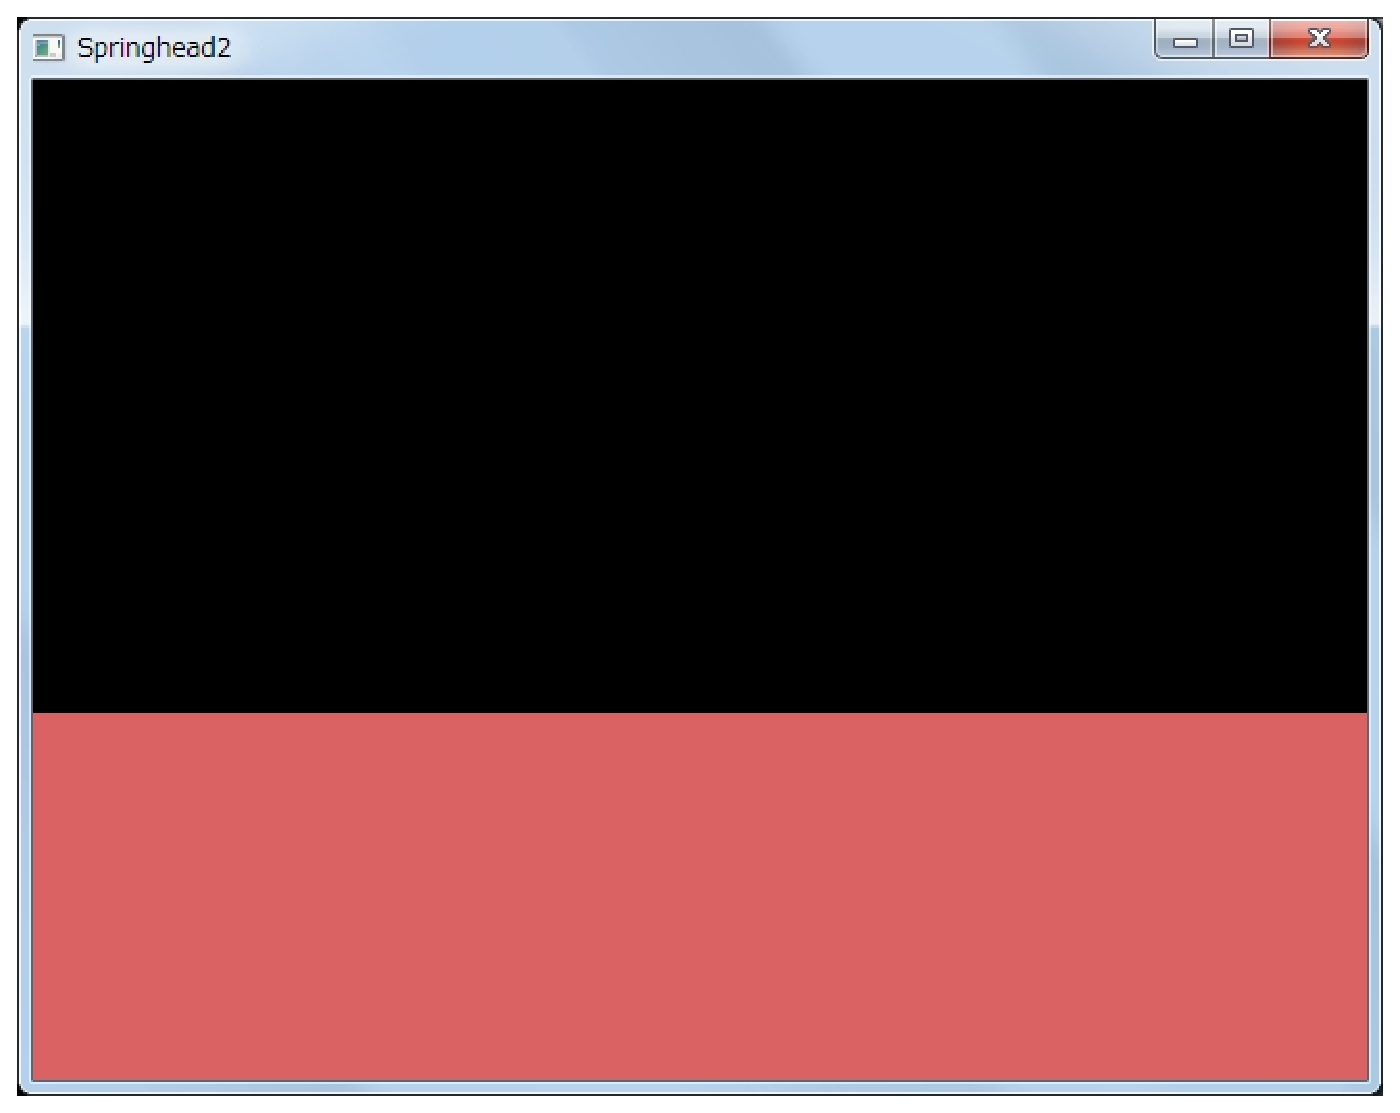
\includegraphics[width=.6\hsize]{fig/newproject8.eps}
\end{center}
\caption{Program running}
\label{fig_newproject8}
\end{figure}

\KLUDGE ビルドするまえにいくつかのプロジェクト設定が必要です.
64\KLUDGE ビットプラットフォームを使用する場合には,プロパティーページの「構成マネージャー」で「\url{x64}\KLUDGE 」プラットフォームを新規作成して選択しておきます.
\KLUDGE また,\ref{libbuild} \KLUDGE で説明したライブラリのビルドは済んでいるものとします.

\KLUDGE まずプロジェクトのプロパティページを開き,構成を「すべての構成」としてください.
\KLUDGE 次に「C/C++ $>$ \KLUDGE 全般 $>$ \KLUDGE 追加のインクルードディレクトリ」に,Fig.\,\ref{fig_newproject4}\KLUDGE のようにSpringhead\KLUDGE のインクルードファイルへのパスを指定してください.
\KLUDGE さらに,「リンカー $>$ \KLUDGE 全般 $>$ \KLUDGE 追加のライブラリディレクトリ」にFig.\,\ref{fig_newproject5}\KLUDGE のようにSpringhead\KLUDGE のライブラリファイルへのパスを指定します (64\KLUDGE ビット構成ぼ場合は \url{win32} \KLUDGE の代わりに \url{win64} \KLUDGE を指定します)\KLUDGE .

\KLUDGE 今度は構成を「Debug\KLUDGE 」にします.
\KLUDGE 「C/C++ $>$ \KLUDGE コード生成 $>$ \KLUDGE ランタイムライブラリ」を「マルチスレッド \KLUDGE デバッグ DLL (\url{/MDd})\KLUDGE 」にします.
\KLUDGE 次に「リンカー $>$ \KLUDGE 入力 $>$ \KLUDGE 追加の依存ファイル」に\url{Springhead14.0DWin32.lib}\KLUDGE を追加してください.

\KLUDGE 最後に構成を「Release\KLUDGE 」に切り替えて同様の設定をします.
\KLUDGE ランタイムライブラリを「マルチスレッド DLL (\url{/MD})\KLUDGE 」として,追加の依存ファイルに\url{Springhead14.0Win32.lib}\KLUDGE を追加します.

\section*{\KLUDGE ビルド・実行}

\KLUDGE 以上で準備完了です.ビルド(F7)\KLUDGE して,実行(F5)\KLUDGE してみてください.
Fig.\,\ref{fig_newproject8}\KLUDGE のような画面が出てくれば成功です.


\chapter{Springhead\KLUDGE の構成}
\label{chap_structure}
\input{structure}

\chapter{Base}
\label{chap_base}
\input{base}

\chapter{Foundation}
\label{chap_foundation}
\index{Foundation}
Foundation\KLUDGE モジュールはすべてのSpringhead\KLUDGE クラスの基本クラスを定義します.
\KLUDGE 普通に使っている限り,ユーザがFoundation\KLUDGE の機能を直接利用することは少ないでしょう.

\section{\KLUDGE 実行時型情報}

\index{IfInfo}
\KLUDGE (ほとんど)すべてのSpringhead\KLUDGE オブジェクトは実行時型情報(RTTI\KLUDGE )を持っています.
C++\KLUDGE にも\texttt{dynamic\_cast}\KLUDGE などのRTTI\KLUDGE 機能がありますが,これよりも大幅にリッチな型情報が提供されます.

\KLUDGE 実行時型情報のクラスは\texttt{IfInfo}\KLUDGE です.
\texttt{IfInfo}\KLUDGE は次節で紹介する\texttt{Object}\KLUDGE クラスから取得できます.

\section{\KLUDGE オブジェクト}

\begin{figure}[t]
\begin{center}
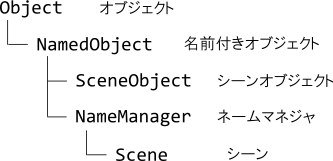
\includegraphics[width=.5\hsize]{fig/utclass.eps}
\end{center}
\caption{Object class hierarchy}
\label{fig_utclass}
\end{figure}

\index{Object}
\KLUDGE ほとんどすべてのSpringhead\KLUDGE オブジェクトは\texttt{Object}\KLUDGE クラスから派生します.
\KLUDGE オブジェクトは複数の子オブジェクトを持つことができます.
Springhead\KLUDGE のデータ構造はオブジェクトが成すツリー構造によって出来上がっています.
Foundation\KLUDGE モジュールにおける\texttt{Object}\KLUDGE からのクラス階層をFig.\,\ref{fig_utclass}\KLUDGE に示します.

\KLUDGE まず\texttt{Object}\KLUDGE クラスの子オブジェクトの作成・管理に関係する関数を紹介します.

\noindent
\begin{tabular}{p{1.0\hsize}}
\\
\texttt{ObjectIf}										\\ \midrule
\texttt{size\_t NChildObject()}							\\
\KLUDGE 子オブジェクトの数を取得する.							\\
														\\
\texttt{ObjectIf* GetChildObject(size\_t pos)}			\\
\texttt{pos}\KLUDGE 番目の子オブジェクトを取得する.			\\
														\\
\texttt{bool AddChildObject(ObjectIf* o)}				\\
\KLUDGE オブジェクト\texttt{o}\KLUDGE を子オブジェクトとして追加する.
\KLUDGE 正しく追加されたら\texttt{true}\KLUDGE ,それ以外は\texttt{false}\KLUDGE を返す.\\
														\\
\texttt{bool DelChildObject(ObjectIf* o)}				\\
\KLUDGE オブジェクト\texttt{o}\KLUDGE を子オブジェクトから削除する.
\KLUDGE 正しく削除されたら\texttt{true}\KLUDGE ,それ以外は\texttt{false}\KLUDGE を返す.\\
														\\
\texttt{void Clear();}									\\
\KLUDGE クリアする.												\\
\\
\end{tabular}

\KLUDGE これらの関数は派生クラスによって実装されますので,追加できる子オブジェクトの種類や数などはクラスごとに異なります.
\KLUDGE また,Springhead\KLUDGE を普通に使用する範囲内ではユーザがこれらの関数を直接呼び出す場面はないでしょう.

\KLUDGE ストリーム出力のために以下の機能があります.

\noindent
\begin{tabular}{p{1.0\hsize}}
\\
\texttt{ObjectIf}										\\ \midrule
\texttt{void Print(std::ostream\& os) const}			\\
\KLUDGE オブジェクトの内容をストリーム\texttt{os}\KLUDGE に出力する.	\\
\\
\end{tabular}
\texttt{Print}\KLUDGE は,基本的にはそのオブジェクトの名前を出力し,子オブジェクトの\texttt{Print}\KLUDGE を再帰的に呼び出します.
\KLUDGE ただし派生クラスによって\texttt{Print}\KLUDGE で出力される内容がカスタマイズされている場合はその限りではありません.

\texttt{NamedObject}\KLUDGE は名前付きオブジェクトです.
\texttt{NamedObject}\KLUDGE の派生クラスには名前を文字列で与えることができ,名前からオブジェクトを検索することができます.
\KLUDGE 名前付きオブジェクトには,直接の親オブジェクト以外に,名前を管理するためのネームマネジャが対応します.

\noindent
\begin{tabular}{p{1.0\hsize}}
\\
\texttt{NamedObjectIf}									\\ \midrule
\texttt{const char* GetName()}			\\
\KLUDGE 名前を取得する.						\\
\\
\texttt{void SetName(const char* n)}	\\
\KLUDGE 名前を設定する.						\\
\\
\texttt{NameManagerIf* GetNameManager()}	\\
\KLUDGE ネームマネジャを取得する.					\\
\\
\end{tabular}

\KLUDGE 名前付きオブジェクトからはさらにシーンオブジェクトが派生します.
\KLUDGE シーンオブジェクトからは周辺モジュールのオブジェクト(\texttt{PHSolid}, \texttt{GRVisual}\KLUDGE など)\KLUDGE が派生します.

\noindent
\begin{tabular}{p{1.0\hsize}}
\\
\texttt{SceneObjectIf}					\\ \midrule
\texttt{SceneIf* GetScene()}			\\
\KLUDGE 自身が所属するシーンを取得する.		\\
\\
\end{tabular}

\section{\KLUDGE ネームマネジャとシーン}

\index{NameManager}
\KLUDGE ネームマネジャは名前付きオブジェクトのコンテナとして働き,それらの名前を管理します.
\KLUDGE また,ネームマネジャはそれ自身名前付きオブジェクトです.

\noindent
\begin{tabular}{p{1.0\hsize}}
\\
\texttt{NameManagerIf}									\\ \midrule
\texttt{NamedObjectIf* FindObject(UTString name)}		\\
\KLUDGE 名前が\texttt{name}\KLUDGE のオブジェクトを検索し,見つかればそのオブジェクトを返す.
\KLUDGE 見つからなければ\texttt{NULL}\KLUDGE を返す.					\\
\\
\end{tabular}


\index{Scene}
\KLUDGE シーンはシーンオブジェクトのコンテナです.
\KLUDGE シーンの基本クラスは\texttt{Scene}\KLUDGE で,ここから各モジュールのシーン(\texttt{PHScene}, \texttt{GRScene}, \texttt{FWScene}\KLUDGE など)\KLUDGE が派生します.
\texttt{Scene}\KLUDGE クラスは特に機能を提供しません.


\section{\KLUDGE タイマ}
\label{sec_uttimer}

\index{UTTimer}
\index{\KLUDGE たいま@\KLUDGE タイマ}
\KLUDGE タイマ機能もFoundation\KLUDGE で提供されます.
\KLUDGE タイマクラスは\texttt{UTTimer}\KLUDGE です.
\KLUDGE タイマを作成するには
\begin{sourcecode}
UTTimerIf* timer = UTTimerIf::Create();
\end{sourcecode}
\KLUDGE とします.\texttt{UTTimer}\KLUDGE には以下のAPI\KLUDGE があります.
\begin{center}
\begin{tabular}{ll}
\texttt{[Get|Set]Resolution}		& \KLUDGE 分解能の取得と設定	\\
\texttt{[Get|Set]Interval}			& \KLUDGE 周期の取得と設定		\\
\texttt{[Get|Set]Mode}				& \KLUDGE モードの取得と設定	\\
\texttt{[Get|Set]Callback}			& \KLUDGE コールバック関数の取得と設定 \\
\texttt{IsStarted}					& \KLUDGE 動いているかどうか	\\
\texttt{IsRunning}					& \KLUDGE コールバック呼び出し中 \\
\texttt{Start}						& \KLUDGE 始動	\\
\texttt{Stop}						& \KLUDGE 停止	\\
\texttt{Call}						& \KLUDGE コールバック呼び出し
\end{tabular}
\end{center}
\texttt{SetMode}\KLUDGE で指定できるモードには以下があります.
\begin{center}
\begin{tabular}{ll}
\texttt{MULTIEDIA}		& \KLUDGE マルチメディアタイマ			\\
\texttt{THREAD}		& \KLUDGE 独立スレッド					\\
\texttt{FRAMEWORK}		& Framework\KLUDGE が提供するタイマ		\\
\texttt{IDLE}			& Framework\KLUDGE が提供するアイドルコールバック
\end{tabular}
\end{center}
\KLUDGE マルチメディアタイマはWindows\KLUDGE が提供する高機能タイマです.
\KLUDGE 独立スレッドモードでは,タイマ用のスレッドが実行され\texttt{Sleep}\KLUDGE 関数により周期が制御されます.
\texttt{FRAMEWORK}\KLUDGE と\texttt{IDLE}\KLUDGE モードを利用するには\texttt{FWApp}\KLUDGE の\texttt{CreateTimer}\KLUDGE 関数を用いる必要があります.
\KLUDGE 基本的に\texttt{FRAMEWORK}\KLUDGE モードではGLUT\KLUDGE のタイマコールバックが使われ,
\texttt{IDLE}\KLUDGE モードではGLUT\KLUDGE のアイドルコールバックが使われます.

Framework\KLUDGE モジュールの\texttt{FWApp}\KLUDGE を利用する場合は,\texttt{FWApp}\KLUDGE の\texttt{CreateTimer}\KLUDGE 関数を利用する方が便利でしょう.


\section{\KLUDGE 状態の保存・再現}
\KLUDGE シミュレーションを行うと、シーンを構成するオブジェクトの状態が変化する。
\KLUDGE ある時刻での状態を保存しておき、再現することができると、数ステップ前に戻ったり、あるステップのシミュレーションを、力を加えた場合と加えない場合で比べたりといった作業ができる。
Springhead\KLUDGE では、\texttt{ObjectStatesIf}\KLUDGE を用いることで、以下のようにシーン全体の状態をまとめてメモリ上に保存、再現することができる。

\begin{sourcecode}
	PHSceneIf* phScene;
	省略:phScene(物理シミュレーションのシーン)の構築
	UTRef<ObjectStatesIf> states;
	states = ObjectStatesIf::Create();	// ObjectStatesオブジェクトの作成
	states->AllocateState(phScene);		// 保存用のメモリ確保
	states->SaveState(phScene);			// 状態の保存
	phScene->Step();					// 仮のシミュレーションを進める
	省略:加速度の取得など
	states->LoadState(phScene);			// 状態の再現
	states->ReleaseState();				// メモリの開放
	省略:力を加えるなどの処理
	phScene->Step();					// 本番のシミュレーションを進める
\end{sourcecode}

\subsection{\KLUDGE 保存・再現のタイミング}
Springhead\KLUDGE のシーン(PHScene\KLUDGE やCRScene)\KLUDGE は、複数のエンジン(PHEngine\KLUDGE やCREngine\KLUDGE の派生クラス)\KLUDGE を呼び出すことで、シミュレーションを進める。
\KLUDGE シーンは、エンジンの呼び出し中以外のタイミングであればいつでも状態を保存・再現することができる。

\subsection{\KLUDGE シーン構成変更の制約}
\KLUDGE 状態保存用のメモリは、シーンの構成に依存している。\texttt{AllocateState(), SaveState(), LoadState()}\KLUDGE だけでなく、\texttt{ObjectStatesIf::ReleaseState()}\KLUDGE も依存するので、\texttt{ObjectIf::AddChildObject()}\KLUDGE などのAPI\KLUDGE によってシーンの構成を変化させてしまうと、保存・再現だけでなくメモリの開放もできなくなる。変更前に開放するか、シーン構成を戻してから開放する必要がある。


\chapter{Collision}
\label{chap_collision}
\section{\KLUDGE 概要}

\index{Collision}
Collision\KLUDGE モジュールは物理計算の基礎となる衝突判定機能を提供します.
\KLUDGE 事実上Collision\KLUDGE モジュールはPhysics\KLUDGE モジュールのサブモジュールとなっており,両者は密接に依存しています.
\KLUDGE ユーザは主として剛体に衝突判定用形状を割り当てる際にCollision\KLUDGE モジュールの機能を利用することになります.

\begin{figure}[t]
\begin{center}
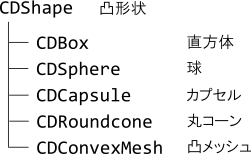
\includegraphics[width=.4\hsize]{fig/cdclass.eps}
\end{center}
\caption{Class hierarchy of Collision module}
\label{fig_cdclass}
\end{figure}

\index{CDShape}
Collision\KLUDGE モジュールのクラス階層をFig.\,\ref{fig_cdclass}\KLUDGE に示します.
\KLUDGE 衝突判定形状はすべて\url{CDShape}\KLUDGE から派生します.
\KLUDGE アルゴリズムの性質上,形状はすべて凸形状でなければなりません.

\section{\KLUDGE 形状の作成}

\KLUDGE 衝突判定形状は次の手順で作成・登録します.
\begin{enumerate}
\item \KLUDGE 形状を作成する
\item \KLUDGE 剛体へ形状を追加する
\item \KLUDGE 形状の位置を設定する
\end{enumerate}
\KLUDGE 以下に順を追って説明します.

\KLUDGE まず形状を作成するには次のようにします.
\begin{sourcecode}
// given PHSdkIf* phSdk

CDBoxDesc desc;
desc.boxsize = Vec3d(1.0, 1.0, 1.0);

CDBoxIf* box = phSdk->CreateShape(desc)->Cast();
\end{sourcecode}
\KLUDGE 衝突判定形状のオブジェクトはPhysics\KLUDGE モジュールが管理します.
\KLUDGE このため,形状を作成するには\url{PHSdk}\KLUDGE クラスの\url{CreateShape}\KLUDGE 関数を使います.
\url{PHSdk}\KLUDGE については\ref{chap_physics}\KLUDGE 章を参照してください.
\KLUDGE 形状を作成するには,まず種類に応じたディスクリプタを作成し,寸法などのパラメータを設定します.
\KLUDGE この例では直方体クラス\url{CDBox}\KLUDGE のディスクリプタを作成して一辺が$1.0$\KLUDGE の立方体を作成します.
\KLUDGE ディスクリプタを指定して\url{CreateShape}\KLUDGE を呼び出すと,対応する種類の形状が作成され,
\KLUDGE そのインタフェースが返されます.
\KLUDGE ただし戻り値は形状の基底クラスである\url{CDShape}\KLUDGE のインタフェースですので,派生クラス(ここでは\url{CDBox}\KLUDGE )のインタフェースを得るには
\KLUDGE 上のように\url{Cast}\KLUDGE 関数で動的キャストする必要があります.

\KLUDGE 形状を作成したら,次にその形状を与えたい剛体に登録します.
\begin{sourcecode}
// given PHSolidIf* solid

solid->AddShape(box);         // first box
\end{sourcecode}
\KLUDGE 剛体クラス\url{PHSolid}\KLUDGE については\ref{chap_physics}\KLUDGE 章を参照してください.
\KLUDGE ここで重要なことは,一度作成した形状は1\KLUDGE つの剛体にいくつでも登録でき,また異なる複数の剛体にも登録できるということです.
\KLUDGE つまり,同じ形状を複数の剛体間で共有することで,形状の作成コストやメモリ消費を抑えることができます.

\url{AddShape}\KLUDGE 関数で登録した直後の形状は,剛体のローカル座標系の原点に位置しています.
\KLUDGE これを変更したい場合は\url{SetShapePose}\KLUDGE 関数を使います.
\begin{sourcecode}
solid->AddShape(box);         // second box
solid->AddShape(box);         // third box 

// move first shape 1.0 in x-direction
solid->SetShapePose(0, Posed(Vec3d(1.0, 0.0, 0.0), Quaterniond());

// rotate second shape 30 degrees along y-axis
solid->SetShapePose(1, Posed(Vec3d(),
                    Quaterniond::Rot(Rad(30.0), 'y')));
\end{sourcecode}
\url{SetShapePose}\KLUDGE の第1\KLUDGE 引数は操作する形状の番号です.最初に\url{AddShape}\KLUDGE した形状の番号が$0$\KLUDGE で,\url{AddShape}\KLUDGE するたびに$1$\KLUDGE 増加します.
\KLUDGE 形状の位置や向きは剛体のローカル座標系で指定します.
\KLUDGE また,形状の位置・向きを取得するには\url{GetShapePose}\KLUDGE 関数を使います.

\KLUDGE 以下ではSpringhead\KLUDGE でサポートされている形状を種類別に解説します.

\subsection*{\KLUDGE 直方体}

\begin{figure}[t]
\begin{center}
\includegraphics[width=.4\hsize]{fig/cdbox.eps}
\end{center}
\caption{Box geometry}
\label{fig_cdbox}
\end{figure}

\index{CDBox}
\index{\KLUDGE ちょくほうたい@\KLUDGE 直方体}
\KLUDGE 直方体(Fig.\,\ref{fig_cdbox})\KLUDGE のクラスは\texttt{CDBox}\KLUDGE です.

\begin{center}
\begin{tabular}{lll}
\multicolumn{3}{l}{\texttt{CDBoxDesc}}					\\ \midrule
\texttt{Vec3f}	&	\texttt{boxsize}	& \KLUDGE 各辺の長さ 	\\
\\
\multicolumn{3}{l}{\texttt{CDBoxIf}}					\\ \midrule
\multicolumn{2}{l}{\texttt{Vec3f GetBoxSize()}}			\\
\multicolumn{2}{l}{\texttt{void SetBoxSize(Vec3f)}}		\\
\end{tabular}
\end{center}


\subsection*{\KLUDGE 球}

\begin{figure}[t]
\begin{center}
\includegraphics[width=.4\hsize]{fig/cdsphere.eps}
\end{center}
\caption{Sphere geometry}
\label{fig_cdsphere}
\end{figure}

\index{CDSphere}
\index{\KLUDGE きゅう@\KLUDGE 球}
\KLUDGE 球(Fig.\,\ref{fig_cdsphere})\KLUDGE のクラスは\url{CDSphere}\KLUDGE です.

\begin{center}
\begin{tabular}{lll}
\multicolumn{3}{l}{\texttt{CDSphereDesc}}				\\ \midrule
\texttt{float}	&	\texttt{radius}	& \KLUDGE 半径 				\\
\\
\multicolumn{3}{l}{\texttt{CDSphereIf}}					\\ \midrule
\multicolumn{2}{l}{\texttt{float GetRadius()}}			\\
\multicolumn{2}{l}{\texttt{void SetRadius(float)}}		\\
\end{tabular}
\end{center}


\subsection*{\KLUDGE カプセル}

\begin{figure}[t]
\begin{center}
\includegraphics[width=.4\hsize]{fig/cdcapsule.eps}
\end{center}
\caption{Capsule geometry}
\label{fig_cdcapsule}
\end{figure}

\index{CDCapsule}
\index{\KLUDGE かぷせる@\KLUDGE カプセル}
\KLUDGE カプセル(Fig.\,\ref{fig_cdcapsule})\KLUDGE のクラスは\url{CDCapsule}\KLUDGE です.
\KLUDGE カプセルは円柱の両端に半球がついた形をしています.

\begin{center}
\begin{tabular}{lll}
\multicolumn{3}{l}{\texttt{CDCapsuleDesc}}				\\ \midrule
\texttt{float}	&	\texttt{radius}	& \KLUDGE 半球の半径 		\\
\texttt{float}	&	\texttt{length} & \KLUDGE 円柱の長さ		\\
\\
\multicolumn{3}{l}{\texttt{CDCapsuleIf}}				\\ \midrule
\multicolumn{2}{l}{\texttt{float GetRadius()}}			\\
\multicolumn{2}{l}{\texttt{void SetRadius(float)}}		\\
\multicolumn{2}{l}{\texttt{float GetLength()}}			\\
\multicolumn{2}{l}{\texttt{void SetLength(float)}}		\\
\end{tabular}
\end{center}


\subsection*{\KLUDGE 丸コーン}

\begin{figure}[t]
\begin{center}
\includegraphics[width=.4\hsize]{fig/cdroundcone.eps}
\end{center}
\caption{Round cone geometry}
\label{fig_cdroundcone}
\end{figure}

\index{CDRoundCone}
\index{\KLUDGE まるこーん@\KLUDGE 丸コーン}
\KLUDGE 丸コーン(Fig.\,\ref{fig_cdroundcone})\KLUDGE のクラスは\url{CDRoundCone}\KLUDGE です.
\KLUDGE 丸コーンはカプセルの両端の半径が非対称になったものです.

\begin{center}
\begin{tabular}{lll}
\multicolumn{3}{l}{\texttt{CDRoundConeDesc}}			\\ \midrule
\texttt{Vec2f}	&	\texttt{radius}	& \KLUDGE 各半球の半径		\\
\texttt{float}	&	\texttt{length} & \KLUDGE 半球間の距離		\\
\\
\multicolumn{3}{l}{\texttt{CDRoundConeIf}}				\\ \midrule
\multicolumn{2}{l}{\texttt{Vec2f GetRadius()}}			\\
\multicolumn{2}{l}{\texttt{void SetRadius(Vec2f)}}		\\
\multicolumn{2}{l}{\texttt{float GetLength()}}			\\
\multicolumn{2}{l}{\texttt{void SetLength(float)}}		\\
\multicolumn{2}{l}{\texttt{void SetWidth(Vec2f)}}		\\
\end{tabular}
\end{center}

\texttt{SetWidth}\KLUDGE 関数は,丸コーンの全長を保存したまま半径を変更します.


\subsection*{\KLUDGE 凸メッシュ}

\begin{figure}[t]
\begin{center}
\includegraphics[width=.4\hsize]{fig/cdconvexmesh.eps}
\end{center}
\caption{Convex mesh geometry}
\label{fig_cdconvexmesh}
\end{figure}

\index{CDConvexMesh}
\index{\KLUDGE とつめっしゅ@\KLUDGE 凸メッシュ}
\KLUDGE 凸メッシュ(Fig.\,\ref{fig_cdconvexmesh})\KLUDGE のクラスは\url{CDConvexMesh}\KLUDGE です.
\KLUDGE 凸メッシュとは凹みや穴を持たない多面体です.
\KLUDGE 頂点座標を指定することで自由な形を作成することができます.

\begin{center}
\begin{tabular}{lll}
\multicolumn{3}{l}{\texttt{CDConvexMeshDesc}}						\\ \midrule
\texttt{vector<Vec3f>}	&	\texttt{vertices}	& \KLUDGE 頂点座標の配列	\\
\\
\multicolumn{3}{l}{\texttt{CDConvexMeshIf}}					\\ \midrule
\multicolumn{2}{l}{\texttt{Vec3f* GetVertices()}}			& \KLUDGE 頂点配列の先頭アドレス	\\
\multicolumn{2}{l}{\texttt{int NVertex()}}					& \KLUDGE 頂点数					\\
\multicolumn{2}{l}{\texttt{CDFaceIf* GetFace(int i)}}		& $i$\KLUDGE 番目の面				\\
\multicolumn{2}{l}{\texttt{int NFace()}}					& \KLUDGE 面数						\\
\end{tabular}
\end{center}

\KLUDGE 凸メッシュが作成される際,\texttt{CDConvexMeshDesc::vertices}\KLUDGE に格納された頂点を内包する最小の凸多面体(凸包)が作成されます.
\KLUDGE 多面体の面を表す\texttt{CDFace}\KLUDGE のインタフェースを以下に示します.

\begin{center}
\begin{tabular}{lll}
\multicolumn{3}{l}{\texttt{CDFaceIf}}						\\ \midrule
\multicolumn{2}{l}{\texttt{int* GetIndices()}}				& \KLUDGE 頂点インデックス配列の先頭アドレス	\\
\multicolumn{2}{l}{\texttt{int NIndex()}}					& \KLUDGE 面の頂点数							\\
\end{tabular}
\end{center}

\texttt{NIndex}\KLUDGE は面を構成する頂点の数を返します(通常$3$\KLUDGE か$4$\KLUDGE です).
\KLUDGE 面は頂点配列を直接保有せず,インデックス配列として間接的に頂点を参照します.
\KLUDGE したがって,面の頂点座標を得るには
\begin{sourcecode}
// given CDConvexMeshIf* mesh
CDFaceIf* face = mesh->GetFace(0);        // get 0-th face
int* idx = face->GetIndices();
Vec3f v = mesh->GetVertices()[idx[0]];    // get 0-th vertex
\end{sourcecode}
\KLUDGE とします.

\section{\KLUDGE 物性の指定}
\label{sec_collision_material}

\index{PHMaterial}
\index{\KLUDGE ぶっせい@\KLUDGE 物性}
\KLUDGE 形状には摩擦係数や跳ね返り係数などの物性を指定することができます.
\KLUDGE 形状の基本クラスである\texttt{CDShape}\KLUDGE のディスクリプタ\texttt{CDShapeDesc}\KLUDGE は\texttt{PHMaterial}\KLUDGE 型の変数\texttt{material}\KLUDGE を持っています.

\begin{center}
\begin{tabular}{lll}
\multicolumn{3}{l}{\texttt{PHMaterial}}							\\ \midrule
\texttt{float}	&	\texttt{density}		& \KLUDGE 密度				\\
\texttt{float}	&	\texttt{mu0}			& \KLUDGE 静止摩擦係数		\\
\texttt{float}	&	\texttt{mu}				& \KLUDGE 動摩擦係数		\\
\texttt{float}	&	\texttt{e}				& \KLUDGE 跳ね返り係数		\\
\texttt{float}	&	\texttt{reflexSpring}	& \KLUDGE 跳ね返りバネ係数(ペナルティ法)	\\
\texttt{float}	&	\texttt{reflexDamper}	& \KLUDGE 跳ね返りダンパ係数(ペナルティ法)\\
\texttt{float}	&	\texttt{frictionSpring}	& \KLUDGE 摩擦バネ係数(ペナルティ法)	\\
\texttt{float}	&	\texttt{frictionDamper}	& \KLUDGE 摩擦ダンパ係数(ペナルティ法)\\
\end{tabular}
\end{center}

\KLUDGE 形状作成後に物性を指定するには\texttt{CDShapeIf}\KLUDGE の関数を使います.

\begin{center}
\begin{tabular}{lll}
\multicolumn{3}{l}{\texttt{CDShapeIf}}						\\ \midrule
\multicolumn{2}{l}{\texttt{void SetDensity(float)}}				& \\
\multicolumn{2}{l}{\texttt{float GetDensity()}}					& \\
\multicolumn{2}{l}{\texttt{void SetStaticFriction(float)}}		& \\
\multicolumn{2}{l}{\texttt{float GetStaticFriction()}}			& \\
\multicolumn{2}{l}{\texttt{void SetDynamicFriction(float)}}		& \\
\multicolumn{2}{l}{\texttt{float GetDynamicFriction()}}			& \\
\multicolumn{2}{l}{\texttt{void SetElasticity(float)}}			& \\
\multicolumn{2}{l}{\texttt{float GetElasticity()}}				& \\
\multicolumn{2}{l}{\texttt{void SetReflexSpring(float)}}		& \\
\multicolumn{2}{l}{\texttt{float GetReflexSpring()}}			& \\
\multicolumn{2}{l}{\texttt{void SetReflexDamper(float)}}		& \\
\multicolumn{2}{l}{\texttt{float GetReflexDamper()}}			& \\
\multicolumn{2}{l}{\texttt{void SetFrictionSpring(float)}}		& \\
\multicolumn{2}{l}{\texttt{float GetFrictionSpring()}}			& \\
\multicolumn{2}{l}{\texttt{void SetFrictionDamper(float)}}		& \\
\multicolumn{2}{l}{\texttt{float GetFrictionDamper()}}			& \\
\end{tabular}
\end{center}

\KLUDGE 物性に基づいた接触力の具体的な計算法については第\ref{sec_physics_contact}\KLUDGE 節を参照して下さい.

\section{\KLUDGE 幾何情報の計算}

\KLUDGE 形状に関する幾何情報を計算する関数を紹介します.

\begin{center}
\begin{tabular}{lll}
\multicolumn{3}{l}{\texttt{CDShapeIf}}							\\ \midrule
\multicolumn{2}{l}{\texttt{float CalcVolume()}}					& \KLUDGE 体積を計算		\\
\multicolumn{2}{l}{\texttt{Vec3f CalcCenterOfMass()}}			& \KLUDGE 質量中心を計算	\\
\multicolumn{2}{l}{\texttt{Matrix3f CalcMomentOfInertia()}}		& \KLUDGE 慣性行列を計算	\\
\end{tabular}
\end{center}

\texttt{CalcVolume}\KLUDGE は形状の体積を計算します.体積に密度(\texttt{GetDensity}\KLUDGE で取得)を掛ければ質量が得られます.
\texttt{CalcCenterOfMass}\KLUDGE 関数は,形状のローカル座標系で表された質量中心の座標を計算します.
\texttt{CalcMomentOfInertia}\KLUDGE 関数は,形状のローカル座標系で表された質量中心に関する慣性行列を計算します.
\KLUDGE ただし,密度を$1$\KLUDGE とした場合の値が返されますので,実際の慣性行列を得るには密度を掛ける必要があります.



\chapter{Physics}
\label{chap_physics}
\section{\KLUDGE 概要}

\index{Physics}
Physics\KLUDGE モジュールは物理シミュレーション機能を提供します.
\KLUDGE 主にサポートされているのは,マルチボディダイナミクスと呼ばれる剛体と関節などの拘束からなる動力学シミュレーションです.
\KLUDGE 今のところソフトボディや流体,パーティクルなどの機能はサポートされていません.

\section{Physics SDK}

\index{PHSdk}
Physics\KLUDGE モジュールのすべてのオブジェクトはSDK\KLUDGE クラス\texttt{PHSdk}\KLUDGE によって管理されます.
\texttt{PHSdk}\KLUDGE クラスは,プログラムの実行を通してただ1つのオブジェクトが存在するシングルトンクラスです.
\texttt{PHSdk}\KLUDGE オブジェクトを作成するには以下のようにします.
\begin{sourcecode}
PHSdkIf* phSdk = PHSdkIf::CreateSdk();
\end{sourcecode}
\KLUDGE 通常この操作はプログラムの初期化時に一度だけ実行します.
\KLUDGE また,Framework\KLUDGE モジュールを使用する場合はユーザが直接\texttt{PHSdk}\KLUDGE を作成する必要はありません.

\texttt{PHSdk}\KLUDGE の機能はシーンと形状の管理です.
\KLUDGE シーンに関する機能は次節で説明します.
\KLUDGE また,形状に関する機能は以下の通りです.

\begin{center}
\begin{tabular}{p{.15\hsize}p{.55\hsize}p{.2\hsize}}
\texttt{PHSdkIf} & &															\\ \midrule
\texttt{CDShapeIf*} & \texttt{CreateShape(const CDShapeDesc\&)}	& \KLUDGE 形状を作成	\\
\texttt{CDShapeIf*}	& \texttt{GetShape(int)}					& \KLUDGE 形状を取得	\\
\texttt{int}		& \texttt{NShape()}							& \KLUDGE 形状の数		\\
\end{tabular}
\end{center}

\KLUDGE 異なるシーン間で形状を共有できるように,形状管理はシーンではなく\texttt{PHSdk}\KLUDGE の機能になっています.
\KLUDGE 詳しくは\ref{chap_collision}\KLUDGE 章を参照してください.

\section{\KLUDGE シーン}
\label{sec_physics_scene}

\index{PHScene}
\KLUDGE シーンは物理シミュレーションを行う環境を表します.
\KLUDGE 複数のシーンを作成できますが,シーン同士は互いに独立しており,ユーザが直接橋渡し処理をしない限りは影響を及ぼしあうことはありません.
\KLUDGE シーンクラスは\texttt{PHScene}\KLUDGE で,\texttt{PHScene}\KLUDGE オブジェクトは\texttt{PHSdk}\KLUDGE により管理されます.

\begin{center}
\begin{tabular}{p{.15\hsize}p{.55\hsize}p{.2\hsize}}
\multicolumn{3}{l}{\texttt{PHSdkIf}}															\\ \midrule
\texttt{PHSceneIf*}	& \texttt{CreateScene(const PHSceneDesc\& desc)}			& \KLUDGE シーンを作成		\\
\texttt{int}		& \texttt{NScene()}											& \KLUDGE シーンの数		\\
\texttt{PHSceneIf*}	& \texttt{GetScene(int i)}									& \KLUDGE シーンを取得		\\
\texttt{void}		& \texttt{MergeScene(PHSceneIf* scene0, PHSceneIf* scene1)}	& \KLUDGE シーンを統合		\\
\end{tabular}
\end{center}

\KLUDGE シーンを作成するには以下のようにします.
\begin{sourcecode}
PHSceneIf* phScene = phSdk->CreateScene();
\end{sourcecode}
\KLUDGE 引数にディスクリプタを指定することもできます.
\texttt{MergeScene}\KLUDGE は,\texttt{scene1}\KLUDGE が保有するオブジェクトをすべて\texttt{scene0}\KLUDGE に移動した後に\texttt{scene1}\KLUDGE を削除します.

\KLUDGE シーンは剛体や関節などの様々な構成要素の管理を行うほか,物理シミュレーションに関する設定を行う機能を提供します.
\KLUDGE 各構成要素の作成についてはそれぞれの節で説明しますので,以下ではシミュレーション設定機能について述べます.

\begin{center}
\begin{tabular}{p{.15\hsize}p{.35\hsize}p{.4\hsize}}
\multicolumn{3}{l}{\texttt{PHSceneDesc}}										\\ \midrule
\texttt{double}		&	\texttt{timeStep}	& \KLUDGE 時間ステップ幅					\\
\texttt{unsigned}	&	\texttt{count}		& \KLUDGE シミュレーションしたステップ数	\\
\texttt{Vec3d}		&	\texttt{gravity}	& \KLUDGE 重力加速度						\\
\texttt{double}		&	\texttt{airResistanceRate}	& \KLUDGE 空気抵抗係数				\\
\texttt{int}		&	\texttt{numIteration}		& LCP\KLUDGE の反復回数				\\
\end{tabular}
\end{center}

\begin{center}
\begin{tabular}{p{.15\hsize}p{.55\hsize}p{.2\hsize}}
\multicolumn{3}{l}{\texttt{PHSceneIf}}							  \\ \midrule
\texttt{double}		& \texttt{GetTimeStep()}					& \\
\texttt{void}		& \texttt{SetTimeStep(double)}				& \\
\texttt{unsigned}	& \texttt{GetCount()}						& \\
\texttt{void}		& \texttt{SetCount(unsigned)}				& \\
\texttt{void}		& \texttt{SetGravity(const Vec3d\&)}		& \\
\texttt{Vec3d}		& \texttt{GetGravity()}						& \\
\texttt{void}		& \texttt{SetAirResistanceRate(double)}		& \\
\texttt{double}		& \texttt{GetAirResistanceRate()}			& \\
\texttt{int}		& \texttt{GetNumIteration()}				& \\
\texttt{void}		& \texttt{SetNumIteration()}				& \\
\end{tabular}
\end{center}

\texttt{timeStep}\KLUDGE は一度のシミュレーションステップで進める時間幅です.
\KLUDGE 小さいほどシミュレーションの精度は上がりますが,同じ時間シミュレーションを進めるのにかかる計算コストは増大します.

\texttt{count}\KLUDGE はシーン作成後にシミュレーションした累積ステップ数です.
\texttt{count}\KLUDGE と\texttt{timeStep}\KLUDGE の積が経過時間を表します.

\texttt{gravity}\KLUDGE は重力加速度ベクトルです.

\texttt{airResistanceRate}\KLUDGE は,シミュレーションの安定性を向上するために毎ステップに各剛体の速度に掛けられる係数です.
\KLUDGE 例えば\texttt{airRegistanceRate}\KLUDGE が$0.95$\KLUDGE であればステップごとに速度が$95$\%\KLUDGE になります.
\KLUDGE このように強制的に減速をかけることで,精度を犠牲に安定性を得ることができます.

\texttt{numIteration}\KLUDGE は,拘束力を計算するために内部で実行されるアルゴリズムの反復回数です.
\KLUDGE 一般に,反復回数に関して指数関数的に拘束力の精度が向上し,計算コストは比例的に増大します.

\subsection*{\KLUDGE シミュレーションの実行}

\KLUDGE シミュレーションを$1$\KLUDGE ステップ進めるには\texttt{Step}\KLUDGE 関数を呼びます.

\begin{center}
\begin{tabular}{p{.15\hsize}p{.3\hsize}p{.45\hsize}}
\multicolumn{3}{l}{\texttt{PHSceneIf}}		\\ \midrule
\texttt{void}	& \texttt{Step()}	& \KLUDGE シミュレーションを$1$\KLUDGE ステップ進める \\
\end{tabular}
\end{center}

\texttt{Step}\KLUDGE を実行すると,おおまかに述べて内部で次の処理が行われます.
\begin{itemize}
\item \KLUDGE 衝突判定と接触拘束の生成
\item \KLUDGE 拘束力の計算
\item \KLUDGE 剛体の速度および位置の更新
\end{itemize}

\section{\KLUDGE 剛体}

\index{PHSolid}
\KLUDGE 剛体は物理シミュレーションの基本要素です.
\KLUDGE 剛体のクラスは\texttt{PHSolid}\KLUDGE です.
\KLUDGE まず剛体を作成・管理するための\texttt{PHScene}\KLUDGE の関数を示します.

\begin{center}
\begin{tabular}{p{.15\hsize}p{.45\hsize}p{.30\hsize}}
\multicolumn{3}{l}{\texttt{PHSceneIf}}									\\ \midrule
\texttt{PHSolidIf*}		& \texttt{CreateSolid(const PHSolidDesc\&)}	& \KLUDGE 剛体を作成する \\
\texttt{int}			& \texttt{NSolids()}						& \KLUDGE 剛体の数 \\
\texttt{PHSolidIf**} 	& \texttt{GetSolids()}						& \KLUDGE 剛体配列の先頭アドレス \\
\end{tabular}
\end{center}

\KLUDGE 剛体を作成するには
\begin{sourcecode}
PHSolidIf* solid = phScene->CreateSolid();
\end{sourcecode}
\KLUDGE とします.ディスクリプタを指定して作成することもできます.
\KLUDGE また,\texttt{GetSolids}\KLUDGE は作成した剛体を格納した内部配列の先頭アドレスを返します.
\KLUDGE したがって,例えば$0$\KLUDGE 番目の剛体を取得するには
\begin{sourcecode}
PHSolidIf* solid = phScene->GetSolids()[0];      // get 0-th solid
\end{sourcecode}
\KLUDGE とします.

\KLUDGE つぎに剛体自身の機能を説明します.

\subsection*{\KLUDGE 物性}

\begin{center}
\begin{tabular}{p{.15\hsize}p{.45\hsize}p{.30\hsize}}
\multicolumn{3}{l}{\texttt{PHSolidDesc}}							\\ \midrule
\texttt{double}		&	\texttt{mass}		& \KLUDGE 質量					\\
\texttt{Matrix3d}	&	\texttt{inertia}	& \KLUDGE 慣性行列				\\
\texttt{Vec3d}		&	\texttt{center}		& \KLUDGE 質量中心				\\
\texttt{bool}		&	\texttt{dynamical}	& \KLUDGE 物理法則にしたがうか	\\
\end{tabular}
\end{center}

\begin{center}
\begin{tabular}{p{.15\hsize}p{.45\hsize}p{.30\hsize}}
\multicolumn{3}{l}{\texttt{PHSolidIf}}								\\ \midrule
\texttt{double}		& \texttt{GetMass()}						& \\
\texttt{double} 	& \texttt{GetMassInv()}						& \\
\texttt{void} 		& \texttt{SetMass(double)}					& \\
\texttt{Vec3d} 		& \texttt{GetCenterOfMass()}				& \\
\texttt{void} 		& \texttt{SetCenterOfMass(const Vec3d\&)}	& \\
\texttt{Matrix3d} 	& \texttt{GetInertia()}						& \\
\texttt{Matrix3d} 	& \texttt{GetInertiaInv()}					& \\
\texttt{void} 		& \texttt{SetInertia(const Matrix3d\&)}		& \\
\texttt{void} 		& \texttt{CompInertia()}					& \\
\texttt{void} 		& \texttt{SetDynamical(bool)}				& \\
\texttt{bool} 		& \texttt{IsDynamical()}					& \\
\end{tabular}
\end{center}

\texttt{GetMassInv}\KLUDGE と\texttt{GetInertiaInv}\KLUDGE はそれぞれ質量の逆数と慣性行列の逆行列を返します.
\texttt{CompInertia}\KLUDGE は,その剛体が持つ形状とそれらの密度をもとに剛体の質量,質量中心と慣性行列を計算し,設定します.
\texttt{dynamical}\KLUDGE は,その剛体が物理法則に従うかどうかを指定するフラグです.
\KLUDGE もし\texttt{dynamical}\KLUDGE が\texttt{true}\KLUDGE の場合,その剛体に加わる力が計算され,
\KLUDGE ニュートンの運動法則にしたがって剛体の速度が変化します.
\KLUDGE 一方,\texttt{dynamical}\KLUDGE が\texttt{false}\KLUDGE の場合は外力による影響を受けず,設定された速度で等速運動します.
\KLUDGE これはちょうど∞の質量をもつ場合と同じです.


\subsection*{\KLUDGE 状態}

\begin{center}
\begin{tabular}{p{.15\hsize}p{.45\hsize}p{.30\hsize}}
\multicolumn{3}{l}{\texttt{PHSolidDesc}}							\\ \midrule
\texttt{Vec3d}	&	\texttt{velocity}		& \KLUDGE 速度					\\
\texttt{Vec3d}	&	\texttt{angVelocity}	& \KLUDGE 角速度				\\
\texttt{Posed}	&	\texttt{pose}			& \KLUDGE 位置と向き			\\
\end{tabular}
\end{center}

\begin{center}
\begin{tabular}{p{.2\hsize}p{.5\hsize}p{.20\hsize}}
\multicolumn{3}{l}{\texttt{PHSolidIf}}									\\ \midrule
\texttt{Vec3d}			& \texttt{GetVelocity()}						& \\
\texttt{void} 			& \texttt{SetVelocity(const Vec3d\&)}			& \\
\texttt{Vec3d} 			& \texttt{GetAngularVelocity()}					& \\
\texttt{void} 			& \texttt{SetAngularVelocity(const Vec3d\&)}	& \\
\texttt{Posed} 			& \texttt{GetPose()}							& \\
\texttt{void} 			& \texttt{SetPose(const Posed\&)}				& \\
\texttt{Vec3d} 			& \texttt{GetFramePosition()}					& \\
\texttt{void} 			& \texttt{SetFramePosition(const Vec3d\&)}		& \\
\texttt{Vec3d} 			& \texttt{GetCenterPosition()}					& \\
\texttt{void} 			& \texttt{SetCenterPosition(const Vec3d\&)}		& \\
\texttt{Quaterniond} 	& \texttt{GetOrientation()}						& \\
\texttt{void} 			& \texttt{SetOrientation(const Quaterniond\&)}	& \\
\end{tabular}
\end{center}

\texttt{velocity}, \texttt{angVelocity}, \texttt{pose}\KLUDGE はそれぞれグローバル座標系に関する剛体の速度,角速度,位置および向きを表します.
\texttt{[Get|Set]FramePosition}\KLUDGE はグローバル座標系に関する剛体の位置を取得/\KLUDGE 設定します.
\KLUDGE これに対して\texttt{[Get|Set]CenterPosition}\KLUDGE は剛体の質量中心の位置を取得/\KLUDGE 設定します.
\KLUDGE 偏心している剛体はローカル座標原点と質量中心が一致しないことに注意してください.
\texttt{[Get|Set]Orientation}\KLUDGE はグローバル座標系に関する剛体の向きを取得/\KLUDGE 設定します.


\subsection*{\KLUDGE 力の印加と取得}

\KLUDGE 剛体に加わる力には
\begin{itemize}
\item \KLUDGE ユーザが設定する外力
\item \KLUDGE 重力
\item \KLUDGE 関節や接触から加わる拘束力
\end{itemize}
\KLUDGE の$3$\KLUDGE 種類があり,それぞれについて並進力とトルクがあります.
\KLUDGE ここで,重力は重力加速度と剛体の質量より決まり,拘束力は拘束条件を満たすように内部で自動的に計算されます.
\KLUDGE 以下ではユーザが剛体に加える外力を設定・取得する方法を示します.

\begin{center}
\begin{tabular}{p{.2\hsize}p{.5\hsize}p{.20\hsize}}
\multicolumn{3}{l}{\texttt{PHSolidIf}}								\\ \midrule
\texttt{void} 	& \texttt{AddForce(Vec3d)}					& \\
\texttt{void} 	& \texttt{AddTorque(Vec3d)}					& \\
\texttt{void} 	& \texttt{AddForce(Vec3d, Vec3d)}			& \\
\texttt{Vec3d} 	& \texttt{GetForce()}						& \\
\texttt{Vec3d} 	& \texttt{GetTorque()}						& \\
\end{tabular}
\end{center}

\KLUDGE 並進力を加えるには\texttt{AddForce}\KLUDGE を使います.
\begin{sourcecode}
solid->AddForce(Vec3d(0.0, -1.0, 0.0));
\end{sourcecode}
\KLUDGE とすると剛体の質量中心に並進力$(0, -1, 0)$\KLUDGE が加わります.ただし力はグローバル座標系で表現されます.
\KLUDGE 一方
\begin{sourcecode}
solid->AddTorque(Vec3d(1.0, 0.0, 0.0));
\end{sourcecode}
\KLUDGE とすると剛体の質量中心に関してモーメント$(1, 0, 0)$\KLUDGE が加わります.
\KLUDGE 作用点を任意に指定するには
\begin{sourcecode}
solid->AddForce(Vec3d(0.0, -1.0, 0.0), Vec3d(0.0, 0.0, 1.0));
\end{sourcecode}
\KLUDGE とします.この場合は並進力$(0, -1, 0)$\KLUDGE が作用点$(0, 0, 1)$\KLUDGE に加わります.
\KLUDGE ここで作用点の位置は剛体のローカル座標ではなくグローバル座標で表現されることに注意してください.
\texttt{AddForce}\KLUDGE や\texttt{AddTorque}\KLUDGE は複数回呼ぶと,それぞれで指定した外力の合力が最終的に剛体に加わる外力となります.

\KLUDGE 外力を取得するには\texttt{GetForce}\KLUDGE ,\texttt{GetTorque}\KLUDGE を使います.
\KLUDGE ただし,これらの関数で取得できるのは直前のシミュレーションステップで剛体に作用した外力です.
\KLUDGE したがって直前のシミュレーションステップ後に\texttt{AddForce}\KLUDGE した力は取得できません.
%\KLUDGE シミュレーションの実行と力の印加,取得に関するフローをFig.\,\ref{fig_addforce}\KLUDGE に示します.


\section{\KLUDGE 関節}

\begin{figure}[t]
\begin{center}
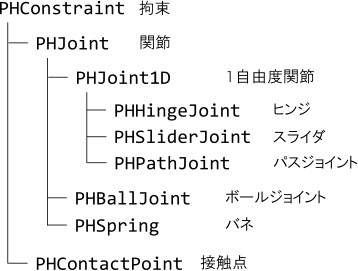
\includegraphics[width=.5\hsize]{fig/phconstraint.eps}
\end{center}
\caption{Constraint class hierarchy}
\label{fig_phconstraint}
\end{figure}

\index{PHConstraint}
\index{PHJoint}
\KLUDGE 拘束とは剛体と剛体の間に作用してその相対的運動に制約を加える要素です.
\KLUDGE 拘束のクラス階層をFig.\,\ref{fig_phconstraint}\KLUDGE に示します.
\KLUDGE まず拘束は関節と接触に分かれます.関節はユーザが作成しますが,接触は衝突判定結果にもとづいて自動的に生成・削除されます.
\KLUDGE 関節はさらにいくつかの種類に分けられます.

\KLUDGE 細かな説明は後回しにして,まずは関節の作成方法から見ていきます.

\subsection*{\KLUDGE 関節の作成}

\KLUDGE 以下ではもっとも使用頻度の高いヒンジの作成を例にとって関節の作成方法を説明します.
\KLUDGE ヒンジを作成するには次のようにします.
\begin{sourcecode}
PHSolidIf* solid0 = phScene->GetSolids()[0];
PHSolidIf* solid1 = phScene->GetSolids()[1];

PHHingeJointDesc desc;
desc.poseSocket.Pos() = Vec3d( 1.0, 0.0, 0.0);
desc.posePlug.Pos()   = Vec3d(-1.0, 0.0, 0.0);
PHHingeJointIf* joint
    = phScene->CreateJoint(solid0, solid1, desc)->Cast();
\end{sourcecode}
\KLUDGE 作成したい関節の種類に応じたディスクリプタを作成し,これを\texttt{PHScene}\KLUDGE の\texttt{CreateJoint}\KLUDGE 関数に渡して関節を作成します.
\KLUDGE このとき,ディスクリプタとともに連結したい剛体のインタフェースも渡します.
\texttt{CreateJoint}\KLUDGE は\texttt{PHJointIf*}\KLUDGE を返しますので,作成した関節のインタフェースを得るには\texttt{Cast}\KLUDGE で動的キャストします.

\KLUDGE 関節に関する\texttt{PHScene}\KLUDGE の関数を以下に示します.

\begin{center}
\begin{tabular}{p{.15\hsize}p{.75\hsize}p{.0\hsize}}
\multicolumn{3}{l}{\texttt{PHSceneIf}}													\\ \midrule
\texttt{PHJointIf*}	& \texttt{CreateJoint(PHSolidIf*, PHSolidIf*, const PHJointDesc\&)}	& \\
\texttt{int}		& \texttt{NJoint()}													& \\
\texttt{PHJointIf*}	& \texttt{GetJoint(int i)}											& \\
\end{tabular}
\end{center}

\texttt{NJoint}\KLUDGE はシーン中の関節の個数を返します.\texttt{GetJoint}\KLUDGE は\texttt{i}\KLUDGE 番目の関節を取得します.


\subsection*{\KLUDGE ソケットとプラグ}

\index{\KLUDGE そけっと@\KLUDGE ソケット}
\index{\KLUDGE ぷらぐ@\KLUDGE プラグ}
\begin{figure}[t]
\begin{center}
\begin{tabular}{c}
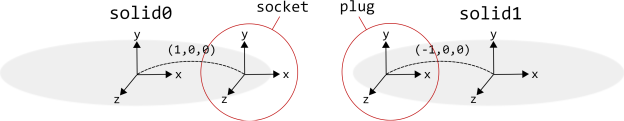
\includegraphics[clip, width=.5\hsize]{fig/socket_plug1.eps} \\
(a) before connection \\
\\
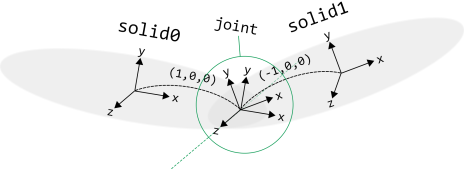
\includegraphics[clip, width=.5\hsize]{fig/socket_plug2.eps} \\
(b) after connection \\
\end{tabular}
\end{center}
\caption{Socket and plug}
\label{fig_socket_plug}
\end{figure}


\KLUDGE さて,上の例でディスクリプタに値を設定している箇所に注目してください.この部分で関節の取り付け位置を指定しています.
Springhead\KLUDGE では,ソケットとプラグと呼ばれるローカル座標系を用いて関節の取り付け位置を表現します.
\KLUDGE ソケットとプラグとは,その名前から連想するように,連結する剛体に取り付ける金具のようなものです.
\texttt{CreateJoint}\KLUDGE の第$1$\KLUDGE 引数の剛体にソケットがつき,第$2$\KLUDGE 引数の剛体にプラグがつきます.
\KLUDGE ソケットとプラグがそれぞれの剛体のどの位置に取り付けられるかを指定するのがディスクリプタの\texttt{poseSocket}\KLUDGE と\texttt{posePlug}\KLUDGE です.
\KLUDGE 上の例ではソケットの位置が$(1,0,0)$\KLUDGE ,プラグの位置が$(-1,0,0)$\KLUDGE でした(Fig.\,\ref{fig_socket_plug}(a))\KLUDGE .
\KLUDGE この場合はFig.\,\ref{fig_socket_plug}(b)\KLUDGE のように剛体が連結されます.
\KLUDGE 後述するように,ヒンジはソケットとプラグのz\KLUDGE 軸を一致させる拘束です.
\KLUDGE したがって連結された剛体同士はソケットとプラグのz\KLUDGE 軸を回転軸として相対的に回転することができます.

\KLUDGE ソケットとプラグに関するディスクリプタとインタフェースを紹介します.

\begin{center}
\begin{tabular}{p{.15\hsize}p{.35\hsize}p{.40\hsize}}
\multicolumn{3}{l}{\texttt{PHConstraintDesc}}					\\ \midrule
\texttt{Posed}	&	\texttt{poseSocket}	& \KLUDGE ソケットの位置と向き	\\
\texttt{Posed}	&	\texttt{posePlug}	& \KLUDGE プラグの位置と向き	\\
\end{tabular}
\end{center}

\begin{center}
\begin{tabular}{p{.15\hsize}p{.50\hsize}p{.25\hsize}}
\multicolumn{3}{l}{\texttt{PHConstraintIf}}								\\ \midrule
\texttt{PHSolidIf*}	& \texttt{GetSocketSolid()}							& \KLUDGE ソケット側の剛体 \\
\texttt{PHSolidIf*} & \texttt{GetPlugSolid()}							& \KLUDGE プラグ側の剛体 \\
\texttt{void} 		& \texttt{GetSocketPose(Posed\&)}					& \\
\texttt{void} 		& \texttt{SetSocketPose(const Posed\&)}				& \\
\texttt{void} 		& \texttt{GetPlugPose(Posed\&)}						& \\
\texttt{void} 		& \texttt{SetPlugPose(const Posed\&)}				& \\
\texttt{void} 		& \texttt{GetRelativePose(Posed\&)}					& \KLUDGE 相対的な位置と向き \\
\texttt{void} 		& \texttt{GetRelativeVelocity(Vec3d\&, Vec3d\&)}	& \KLUDGE 相対速度 \\
\texttt{void} 		& \texttt{GetConstraintForce(Vec3d\&, Vec3d\&)}		& \KLUDGE 拘束力 \\
\end{tabular}
\end{center}
%	Vec3d GetMotorf();
%	Vec3d GetLimitf();

\texttt{GetRelativePose}\KLUDGE はソケット座標系から見たプラグ座標系の相対的な位置と向きを取得します.
\KLUDGE 同様に,\texttt{GetRelativeVelocity}\KLUDGE はソケットからみたプラグの相対速度をソケット座標系で取得します.
\KLUDGE ここで第$1$\KLUDGE 引数が並進速度,第$2$\KLUDGE 引数が角速度です.
\texttt{GetConstraintForce}\KLUDGE はこの拘束が剛体に加えた拘束力を取得します(\KLUDGE 第$1$\KLUDGE 引数が並進力,第$2$\KLUDGE 引数がモーメント)\KLUDGE .
\KLUDGE 具体的には,ソケット側剛体に作用した拘束力をソケット座標系で表現したものが得られます.
\KLUDGE プラグ側剛体には作用反作用の法則によって逆向きの力が作用しますが,これを直接取得する関数は用意されていません.





% --- --- --- --- --- --- --- --- --- --- --- --- --- --- ---
\subsection*{\KLUDGE 関節の種類}

Springhead\KLUDGE で使用可能な関節の種類は

\begin{itemize}
\item \KLUDGE ヒンジ (\texttt{PHHingeIf})
\item \KLUDGE スライダ (\texttt{PHSliderIf})
\item \KLUDGE パスジョイント (\texttt{PHPathJointIf})
\item \KLUDGE ボールジョイント (\texttt{PHBallJointIf})
\item \KLUDGE バネ (\texttt{PHSpringIf})
\end{itemize}

\KLUDGE の5\KLUDGE 種類です.種類ごとに,自由度・拘束の仕方・変位の求め方が異なります.


% --- --- --- --- ---
\subsubsection*{\KLUDGE ヒンジ}

\begin{fig}
\epscapopt{phhingejoint}{Hinge joint}{width=0.5\hsize}
\end{fig}

\index{PHHingeJoint}
\index{\KLUDGE ひんじ@\KLUDGE ヒンジ}
\KLUDGE ヒンジは$1$\KLUDGE 軸回転関節です.
\KLUDGE ヒンジは,\Fig{phhingejoint}\KLUDGE に示すようにソケットとプラグのz\KLUDGE 軸が一致するように拘束します.
\KLUDGE このときソケットのy\KLUDGE 軸とプラグのy\KLUDGE 軸の成す角(x\KLUDGE 軸同士でも同じことですが)\KLUDGE が関節変位となります.

\KLUDGE 関節変位を取得するAPI\KLUDGE は$1$\KLUDGE 自由度関節(\texttt{PH1DJointIf})\KLUDGE で共通です.そのためヒンジに限らずスライダ・パスジョイントでも使用できます.

\begin{reference}{PH1DJointIf}
\classmember{double GetPosition()}
\KLUDGE 関節の変位を取得します.変位のはかり方は関節の種類に依存します.
\end{reference}

% --- --- --- --- ---
\subsubsection*{\KLUDGE スライダ}

\begin{fig}
\epscapopt{phsliderjoint}{Slider joint}{width=0.5\hsize}
\end{fig}

\index{PHSliderJoint}
\index{\KLUDGE すらいだ@\KLUDGE スライダ}
\KLUDGE スライダは$1$\KLUDGE 自由度の直動関節です.
\KLUDGE スライダは,\Fig{phsliderjoint}\KLUDGE に示すようにソケットとプラグのz\KLUDGE 軸が同一直線上に乗り,かつ両者のx\KLUDGE 軸,y\KLUDGE 軸が同じ向きを向くように拘束します.
\KLUDGE このときソケットの原点からプラグの原点までが関節変位となります.



% --- --- --- --- ---
\subsubsection*{\KLUDGE パスジョイント}

\index{PHPathJoint}
\index{\KLUDGE ぱすじょいんと@\KLUDGE パスジョイント}
\KLUDGE パスジョイントはソケットとプラグの相対位置関係を$1$\KLUDGE パラメータの自由曲線で表現する関節です.詳しくは後述します.

T.B.D.



% --- --- --- --- ---
\subsubsection*{\KLUDGE ボールジョイント}

\begin{fig}
  \begin{tabular}{cc}
    \epsopt{phballjoint}{width=0.45\hsize} & \epsopt{swingtwist}{width=0.35\hsize} \\
    (a) & (b)
  \end{tabular}
  \labelcap{phballjoint}{Ball Joint}
\end{fig}

\index{PHBallJoint}
\index{\KLUDGE ぼーるじょいんと@\KLUDGE ボールジョイント}
\KLUDGE ボールジョイントは$3$\KLUDGE 自由度の回転関節です.
\KLUDGE ボールジョイントは\Fig{phballjoint}(a)\KLUDGE に示すようにソケットとプラグの原点が一致するように拘束します.
\KLUDGE ソケット座標系をプラグ座標系に変換するようなクォータニオンが変位となります.

\KLUDGE 一方で,ボールジョイントの変位はオイラー角の一種であるSwing-Twist\KLUDGE 座標系(\Fig{phballjoint}(b))\KLUDGE で取得することもできます.
\KLUDGE ソケットとプラグのz\KLUDGE 軸同士がなす角をスイング角(Swing)\KLUDGE ,プラグのz\KLUDGE 軸をソケットのx-y\KLUDGE 平面への射影がソケットのx\KLUDGE 軸となす角をスイング方位角(Swing-Dir)\KLUDGE ,プラグのz\KLUDGE 軸周りの回転角度をツイスト角(Twist)\KLUDGE と呼びます.Swing-Twist\KLUDGE 座標系は,後述するボールジョイントの関節可動範囲の指定に用います.

\KLUDGE この2\KLUDGE 種類の変位は,それぞれに対応した関数で取得することができます.
\begin{reference}{PHBallJoint}
\classmember{Quaterniond GetPosition()}
\KLUDGE ソケット座標系をプラグ座標系に変換するようなクォータニオンを返します.

\classmember{Vec3d GetAngle()}
Swing-Twist\KLUDGE 座標系で表現された関節変位を返します.
\end{reference}


\subsubsection*{\KLUDGE バネ}

\index{PHSpring}
\index{\KLUDGE ばね@\KLUDGE バネ}

\begin{fig}
\epscapopt{phspring}{Spring}{width=0.5\hsize}
\end{fig}

\KLUDGE 剛体間を連結するダンパ付きバネです.ソケット座標系とプラグ座標系が一致するときが自然状態で,位置の変位・姿勢の変位に比例して自然状態に戻すような力・モーメントを発生します.並進運動に作用するバネ・ダンパ係数と,回転運動に作用するバネ・ダンパ係数はディスクリプタによってそれぞれ設定できます.

\begin{lightreference}{PHSpringDesc}
% \member\KLUDGE マクロがうまく機能しない
%\member{Vec3d spring}{\KLUDGE 並進運動に対するバネ係数}
%\member{Vec3d damper}{\KLUDGE 並進運動に対するダンパ係数}
%\member{double springOri}{\KLUDGE 回転運動に対するバネ係数}
%\member{double damperOri}{\KLUDGE 回転運動に対するダンパ係数}
\multicolumn{2}{l}{\texttt{Vec3d spring}} & \KLUDGE 並進運動に対するバネ係数 \\
\multicolumn{2}{l}{\texttt{Vec3d damper}} & \KLUDGE 並進運動に対するダンパ係数 \\
\multicolumn{2}{l}{\texttt{double springOri}} & \KLUDGE 回転運動に対するバネ係数 \\
\multicolumn{2}{l}{\texttt{double damperOri}} & \KLUDGE 回転運動に対するダンパ係数 \\
\end{lightreference}


\subsection*{\KLUDGE 有効化と無効化}

\begin{center}
\begin{tabular}{p{.15\hsize}p{.45\hsize}p{.30\hsize}}
\multicolumn{3}{l}{\texttt{PHConstraintDesc}}					\\ \midrule
\texttt{bool}	&	\texttt{bEnabled}	& \KLUDGE 有効/\KLUDGE 無効フラグ		\\
\end{tabular}
\end{center}

\begin{center}
\begin{tabular}{p{.15\hsize}p{.50\hsize}p{.25\hsize}}
\multicolumn{3}{l}{\texttt{PHConstraintIf}}						\\ \midrule
\texttt{void}	& \texttt{Enable(bool)}					& \\
\texttt{bool} 	& \texttt{IsEnabled()}					& \\
\end{tabular}
\end{center}

\KLUDGE 有効な拘束は拘束力を生じます.無効化された拘束は存在しないのと同じ状態になりますが,
\KLUDGE 削除するのと異なりいつでも再度有効化することができます.
\KLUDGE 作成直後の拘束は有効化されています.





\subsection*{\KLUDGE 関節制御}

\subsubsection*{$1$\KLUDGE 自由度関節の場合}

\begin{center}
\begin{tabular}{p{.15\hsize}p{.45\hsize}p{.30\hsize}}
\multicolumn{3}{l}{\texttt{PHJoint1DDesc}}								\\ \midrule
\texttt{double}	&	\texttt{spring}			& \KLUDGE 可動範囲下限				\\
\texttt{double}	&	\texttt{damper}			& \KLUDGE 可動範囲上限				\\
\texttt{double}	&	\texttt{targetPosition}	& \KLUDGE 可動範囲制限用バネ係数	\\
\texttt{double}	&	\texttt{targetVelocity}	& \KLUDGE 可動範囲制限用ダンパ係数	\\
\texttt{double}	&	\texttt{offsetForce}	& \\
\texttt{double}	&	\texttt{fMax}			& \\
\end{tabular}
\end{center}

\begin{center}
\begin{longtable}{p{.15\hsize}p{.45\hsize}p{.30\hsize}}
\multicolumn{3}{l}{\texttt{PHJoint1DIf}}						\\ \midrule
\texttt{double}	& \texttt{GetPosition()}				& \KLUDGE 関節変位を取得 \\
\texttt{double} & \texttt{GetVelocity()}				& \KLUDGE 関節速度を取得 \\
\texttt{void} 	& \texttt{SetSpring(double)}			& \\
\texttt{double} & \texttt{GetSpring()}					& \\
\texttt{void} 	& \texttt{SetDamper(double)}			& \\
\texttt{double} & \texttt{GetDamper()}					& \\
\texttt{void} 	& \texttt{SetTargetPosition(double)}	& \\
\texttt{double} & \texttt{GetTargetPosition()}			& \\
\texttt{void} 	& \texttt{SetTargetVelocity(double)}	& \\
\texttt{double} & \texttt{GetTargetVelocity()}			& \\
\texttt{void} 	& \texttt{SetOffsetForce(double)}		& \\
\texttt{double} & \texttt{GetOffsetForce()}				& \\
\texttt{void} 	& \texttt{SetTorqueMax(double)}			& \KLUDGE 最大関節トルクを設定 \\
\texttt{double} & \texttt{GetTorqueMax()}				& \KLUDGE 最大関節トルクを取得 \\
\end{longtable}
\end{center}

\KLUDGE 関節を駆動する力$f$\KLUDGE は次式で与えられます.
\begin{align*}
f = K(p_0 - p) + D(v_0 - v) + f_0
\end{align*}
\KLUDGE ここで$p$\KLUDGE ,$v$\KLUDGE はそれぞれ関節変位と関節速度で\texttt{GetPosition}\KLUDGE ,\texttt{GetVelocity}\KLUDGE で取得できます.
\KLUDGE その他の記号とディスクリプタ変数との対応は以下の通りです.
\begin{center}
\begin{tabular}{ll}
$K$		&	\texttt{spring}				\\
$D$		&	\texttt{damper}				\\
$p_0$	&	\texttt{targetPosition}		\\
$v_0$	&	\texttt{targetVelocity}		\\
$f_0$	&	\texttt{offsetForce}
\end{tabular}
\end{center}
\KLUDGE 上の式はバネ・ダンパモデルとPD\KLUDGE 制御則の二通りの解釈ができます.
\KLUDGE 前者としてとらえるなら$K$\KLUDGE はバネ係数,$D$\KLUDGE はダンパ係数,$p_0$\KLUDGE はバネの自然長,$v_0$\KLUDGE は基準速度となります.
\KLUDGE 後者としてとらえる場合は$K$\KLUDGE はP\KLUDGE ゲイン,$D$\KLUDGE はD\KLUDGE ゲイン,$p_0$\KLUDGE は目標変位,$v_0$\KLUDGE は目標速度となります.
\KLUDGE また,$f_0$\KLUDGE は関節トルクのオフセット項です.
\KLUDGE 上の式で得られた関節トルクは最後に$\pm$\texttt{fMax}\KLUDGE の範囲に収まるようにクランプされます.

\subsubsection*{\KLUDGE ボールジョイントの場合}

\KLUDGE ヒンジと同様に,バネダンパモデル・PD\KLUDGE 制御を実現します.
\KLUDGE ボールジョイントの変位はクォータニオンで表されるため,目標変位\texttt{targetPosition}\KLUDGE はクォータニオンで,目標速度\texttt{targetVelocity}\KLUDGE は回転ベクトルで与えます.

\begin{lightreference}{PHBallJointDesc}
% \member\KLUDGE マクロがうまく機能しない
%\member{double spring}{\KLUDGE バネ係数}
%\member{double damper}{\KLUDGE ダンパ係数}
%\member{Quaterniond targetPosition}{\KLUDGE 目標変位}
%\member{Vec3d targetVelocity}{\KLUDGE 目標速度}
%\member{Vec3d offsetForce}{\KLUDGE モータートルク}
%\member{double fMax}{\KLUDGE 関節トルクの限度}
\multicolumn{2}{l}{\texttt{double spring}} & \KLUDGE バネ係数 \\
\multicolumn{2}{l}{\texttt{double damper}} & \KLUDGE ダンパ係数 \\
\multicolumn{2}{l}{\texttt{Quaterniond targetPosition}} & \KLUDGE 目標変位 \\
\multicolumn{2}{l}{\texttt{Vec3d targetVelocity}} & \KLUDGE 目標速度 \\
\multicolumn{2}{l}{\texttt{Vec3d offsetForce}} & \KLUDGE モータートルク \\
\multicolumn{2}{l}{\texttt{double fMax}} & \KLUDGE 関節トルクの限度 \\
\end{lightreference}



	%\multicolumn{2}{l}{\texttt{void SetMotorTorque(double)}}		& \\
	%\multicolumn{2}{l}{\texttt{double GetMotorTorque()}}	& \\

	%double	secondDamper;	///< \KLUDGE 二個目のダンパ係数
	%double  yieldStress;	///< \KLUDGE 降伏応力
	%double  hardnessRate;	///< \KLUDGE 降伏応力以下の場合に二個目のダンパ係数に掛ける比率

	%void SetTrajectoryVelocity(double v);
	%double GetTrajectoryVelocity();
	%double  GetSecondDamper();
	%void	SetSecondDamper(double input);
	%double GetYieldStress();
    %void SetYieldStress(const double yS);
	%double GetHardnessRate();
	%void SetHardnessRate(const double hR);
	%PHJointDesc::PHDeformationType 	GetDeformationMode();





% --- --- --- --- --- --- --- --- --- --- --- --- --- --- ---
\subsection*{\KLUDGE 可動域制限}

\texttt{CreateLimit}\KLUDGE は可動範囲制約オブジェクトのディスクリプタを引数にとります.
$1$\KLUDGE 自由度関節の可動範囲制約の場合,\texttt{Vec2d range}\KLUDGE が可動域を表します.\texttt{range[0]}\KLUDGE が可動域の下限,\texttt{range[1]}\KLUDGE が上限です.\texttt{range[0] < range[1]}\KLUDGE が満たされているときに限り可動範囲制約が有効となります.
\KLUDGE デフォルトでは\texttt{range[0] > range[1]}\KLUDGE となる値が設定されていて,可動範囲制約は無効となっています.

\KLUDGE 関節の変位が可動範囲限界に到達したとき,範囲を超過しないように可動範囲制約の拘束力が作用します.
\KLUDGE このとき,関節変位を範囲内に押し戻す力はバネ・ダンパモデルで計算されます.
\KLUDGE このバネ係数とダンパ係数はそれぞれディスクリプタの\texttt{spring}\KLUDGE ,\texttt{damper}\KLUDGE で指定します.

\begin{tips}
\KLUDGE 可動範囲用の\texttt{spring}\KLUDGE ,\texttt{damper}\KLUDGE は初期値でも十分大きな値が設定されていますが,関節制御において非常に大きなバネ・ダンパ係数を用いると可動範囲制約のバネ・ダンパが負けてしまうことがあります.その場合には関節制御より大きな係数を適切に再設定すると,可動範囲内で関節を制御する事ができるようになります.
\end{tips}


\subsubsection*{$1$\KLUDGE 自由度関節の場合}

\begin{reference}{PH1DJointLimitDesc}
\classmember{Vec2d range}
\KLUDGE 可動範囲を表します.\texttt{range[0]}\KLUDGE が下限,\texttt{range[1]}\KLUDGE が上限です.

\classmember{double spring} \Plus
\classmember{double damper}
\KLUDGE 可動範囲を制限するためのバネ・ダンパモデルの係数です.
\end{reference}

\begin{reference}{PH1DJointLimitIf}
\classmember{IsOnLimit()}
\KLUDGE 現在の関節姿勢が可動範囲外にある時に\texttt{true}\KLUDGE を返します.この関数が\texttt{true}\KLUDGE を返すような時,関節には可動域制約を実現するための拘束力が発生しています.
\end{reference}


\subsubsection*{\KLUDGE ボールジョイントの場合}

\KLUDGE ボールジョイントの可動範囲は\Fig{phballjoint}(b)\KLUDGE に示すSwing-Twist\KLUDGE 座標系によって指定します.

\KLUDGE ボールジョイントに対しては2\KLUDGE 種類の可動範囲制約を使用することができます.
\begin{itemize}
\item \texttt{ConeLimit}\KLUDGE は円錐形の可動範囲制約で,主に関節のスイング角を一定範囲内に制約します.
\item \texttt{SplineLimit}\KLUDGE は自由曲線形の可動範囲制約で,プラグ座標系z\KLUDGE 軸の可動範囲を閉曲線で指定することができます.
\end{itemize}

\KLUDGE ここでは\texttt{ConeLimit}\KLUDGE について説明します(\texttt{SplineLimit}\KLUDGE については後述します)\KLUDGE .

\begin{reference}{PHBallJointConeLimitDesc}
\classmember{Vec2d limitSwing}
\KLUDGE スイング角の可動範囲です.概念的には,関節が一定以上に折れ曲がらないようにする制約です(\KLUDGE スイング角の下限を設定する事もできるので,実際には一定以上にまっすぐにならないようにする機能も有しています)\KLUDGE .

\texttt{limitSwing[0]}\KLUDGE が下限,\texttt{limitSwing[1]}\KLUDGE が上限です.\texttt{limitSwing}\KLUDGE を取得・設定するためのAPI\KLUDGE は
\begin{quote}
\texttt{PHBallJointConeLimitIf::[Set|Get]SwingRange(range)}
\end{quote}
\KLUDGE です.

\texttt{limitSwing[0] > limitSwing[1]}\KLUDGE となる時は無効化されます.デフォルトでは\texttt{limitSwing[0] > limitSwing[1]}\KLUDGE となる値がセットされています.

\classmember{Vec2d limitTwist}
\KLUDGE ツイスト角の可動範囲です.概念的には,関節が一定以上にねじれないようにするための制約です.

\texttt{limitTwist[0]}\KLUDGE が下限,\texttt{limitTwist[1]}\KLUDGE が上限です.\texttt{limitTwist}\KLUDGE を取得・設定するためのAPI\KLUDGE は
\begin{quote}
\texttt{PHBallJointConeLimitIf::[Set|Get]TwistRange(range)}
\end{quote}
\KLUDGE です.

\texttt{limitTwist[0] > limitTwist[1]}\KLUDGE となる時は無効化されます.デフォルトでは\texttt{limitTwist[0] > limitTwist[1]}\KLUDGE となる値がセットされています.

\classmember{double spring} \Plus
\classmember{double damper}
\KLUDGE 可動範囲を制限するためのバネ・ダンパモデルの係数です.$1$\KLUDGE 自由度関節の場合と同じです.
\end{reference}

\begin{reference}{PHBallJointConeLimitIf}
\classmember{IsOnLimit()}
\KLUDGE 現在の関節姿勢が可動範囲外にある時に\texttt{true}\KLUDGE を返します.$1$\KLUDGE 自由度関節の場合と同じです.
\end{reference}



% --- --- --- --- --- --- --- --- --- --- --- --- --- --- ---
\subsection*{\KLUDGE ボールジョイントの自由曲線可動域} \label{sec_splinelimit}





% --- --- --- --- --- --- --- --- --- --- --- --- --- --- ---
\subsection*{\KLUDGE パスジョイント} \label{sec_phpathjoint}



% --- --- --- --- --- --- --- --- --- --- --- --- --- --- ---
\subsection*{\KLUDGE 弾塑性変形バネダンパ}







\section{\KLUDGE 関節系の逆運動学}

% ----- ----- ----- ----- ----- ----- ----- ----- ----- ----- ----- ----- ----- ----- ----- ----- ----- -----
%
% \KLUDGE 概説
% 

\KLUDGE 逆運動学(IK)\KLUDGE は,剛体関節系において剛体が目標位置に到達するよう関節を制御する機能です.

Springhead\KLUDGE では,関節系のヤコビアンを用いたIK\KLUDGE 機能が使用可能です.
\KLUDGE 物理シミュレーションの1\KLUDGE ステップごとに関節系のヤコビアンを計算し,それに基づいて剛体を目標位置・姿勢に近づけるような各関節の角速度を計算します.
\KLUDGE シミュレーションを続けることで,最終的に剛体が目標位置・姿勢となった状態が得られます.

Springhead\KLUDGE 上の剛体関節系に対してIK\KLUDGE を使用するには,少々下準備が必要です.
\KLUDGE 次のように3\KLUDGE つの剛体が直線状につながった関節系を例にとって解説します.

\begin{center}
\epsopt{ikexample3link}{width=0.5\hsize}
\end{center}


% ----- ----- ----- ----- ----- ----- ----- ----- ----- ----- ----- ----- ----- ----- ----- ----- ----- -----
%
% \KLUDGE 例
% 

IK\KLUDGE を使用するには,まずIK\KLUDGE に用いるための関節を「アクチュエータ」として登録する必要があります.
\begin{sourcecode}
// given PHSceneIf* phScene
// given PHSolidIf* solid1, solid2, solid3
// given PHHingeJointIf* joint1 (solid1 <-> solid2)
// given PHHingeJointIf* joint2 (solid2 <-> solid3)

PHIKHingeActuatorDesc descIKActuator;

PHIKHingeActuatorIf* ikActuator1
  = phScene->CreateIKActuator(descIKActuator);
ikActuator1.AddChildObject(joint1);

PHIKHingeActuatorIf* ikActuator2
  = phScene->CreateIKActuator(descIKActuator);
ikActuator1.AddChildObject(joint2);
\end{sourcecode}
\texttt{PHIKHingeActuatorIf}\KLUDGE は\texttt{PHHingeJointIf}\KLUDGE に対応するアクチュエータクラスです.


\KLUDGE 次に,関節系の親子関係を登録します.親アクチュエータに,子アクチュエータを登録します.
\begin{sourcecode}
ikActuator1.AddChildObject(ikActuator2);
\end{sourcecode}


\KLUDGE また,IK\KLUDGE を用いて到達させる先端の剛体を「エンドエフェクタ」として登録する必要があります.
\begin{sourcecode}
PHIKEndEffectorDesc descEndEffector;

PHIKEndEffectorIf* ikEndEffector1
  = phScene->CreateIKEndEffector(descEndEffector);
ikEndEffector1.AddChildObject(solid3);
\end{sourcecode}


\KLUDGE 最後に,剛体関節系の親子関係において,エンドエフェクタの直接の親にあたるアクチュエータに対し,エンドエフェクタを登録します.
\begin{sourcecode}
ikActuator2.AddChildObject(ikEndEffector1);
\end{sourcecode}
\KLUDGE この例では \texttt{solid1 -(joint1)-> solid2 -(joint2)-> solid3} \KLUDGE のように関節が接続されていますから,関節系の末端である \texttt{solid3} \KLUDGE をエンドエフェクタにした場合,直接の親にあたるアクチュエータは \texttt{joint2} \KLUDGE に対応するアクチュエータ,すなわち \texttt{ikActuator2} \KLUDGE ということになります.

\KLUDGE ここまでの作業で,生成されたオブジェクトの関係は以下のようになっているはずです.
\begin{center}
\epsopt{ikexample3linkobjects}{width=0.9\hsize}
\end{center}
\KLUDGE これで下準備は終わりです.

\KLUDGE 目標位置をセットし,IK\KLUDGE エンジンを有効にするとIK\KLUDGE が動き始めます.
\begin{sourcecode}
// solid3 goes to (2, 5, 0)
ikEndEffector1->SetTargetPosition(Vec3d(2, 5, 0)); 

phScene->GetIKEngine()->Enable(true);

...
phScene->Step(); // IK is calculated in physics step
...
\end{sourcecode}

% ----- ----- ----- ----- ----- ----- ----- ----- ----- ----- ----- ----- ----- ----- ----- ----- ----- -----
%
% \KLUDGE 詳細
% 

% ----- ----- ----- ----- ----- ----- ----- ----- ----- ----- ----- ----- ----- ----- ----- ----- 
\subsection*{IK\KLUDGE エンジン}
% \KLUDGE 概説

IK\KLUDGE の計算は,\texttt{PHScene}\KLUDGE が持つIK\KLUDGE エンジン(\texttt{PHIKEngine})\KLUDGE によって実現されています.

IK\KLUDGE エンジンはデフォルトでは無効となっています.
\begin{sourcecode}
phScene->GetIKEngine()->Enable(true);
\end{sourcecode}
\KLUDGE を実行することで有効となります.\texttt{GetIKEngine()}\KLUDGE は,\texttt{PHScene}\KLUDGE が持つIK\KLUDGE エンジンを取得するAPI\KLUDGE です.

Springhead\KLUDGE におけるIK\KLUDGE の計算原理は,関節系のヤコビ行列(ヤコビアン)に基づきます.全アクチュエータの関節角度に微小変化量 $\varDelta\bm{\theta}$ \KLUDGE を与えた時の,全エンドエフェクタの位置の微小変化量 $\varDelta\bm{r}$ \KLUDGE は,関節系のヤコビアン $J$ \KLUDGE を用いて
\[
\varDelta\bm{r} = J \varDelta\bm{\theta}
\]
\KLUDGE と表されます.毎ステップごとに関節系ヤコビアン$J$\KLUDGE および目標位置に向かう微小変位$\varDelta\bm{r}$\KLUDGE を計算し,上記の線形連立方程式を解くことで各関節に与える角速度を求めます.

\KLUDGE 線形連立方程式の求解にはガウス=\KLUDGE ザイデル法による繰り返し解法を用いています.そのため1\KLUDGE ステップあたりの繰り返し計算の回数によって計算速度と計算精度のトレードオフがあります.繰り返しの回数は,
\begin{sourcecode}
// 20 iteration per 1 physics step
phScene->GetIKEngine()->SetNumIter(20);
\end{sourcecode}
\KLUDGE のようにして設定することができます.

% ----- ----- ----- ----- ----- ----- ----- ----- ----- ----- ----- ----- ----- 
% \KLUDGE リファレンス
\referencetitle

\begin{reference}{PHSceneIf}
\classmember{PHIKEngineIf* GetIKEngine()}
IK\KLUDGE エンジンを取得します.
\end{reference}

\begin{reference}{PHIKEngineIf}
\classmember{Enable(bool b)}
IK\KLUDGE エンジンの有効・無効を切り替えます.引数が\texttt{true}\KLUDGE ならば有効化し,\texttt{false}\KLUDGE ならば無効化します.

\classmember{SetNumIter(int n)}
IK\KLUDGE の繰り返し計算回数を1\KLUDGE ステップあたり\texttt{n}\KLUDGE 回にセットします.
\end{reference}



% ----- ----- ----- ----- ----- ----- ----- ----- ----- ----- ----- ----- ----- ----- ----- ----- 
\subsection*{\KLUDGE アクチュエータ}
% \KLUDGE 概説

Springhead\KLUDGE では,IK\KLUDGE に使用する各関節をアクチュエータと呼びます.IK\KLUDGE は,アクチュエータを駆動させて剛体を目標位置に到達させます.

\KLUDGE <オブジェクト関係図>

IK\KLUDGE エンジンはアクチュエータを複数保持し,各アクチュエータが各関節を保持します.アクチュエータオブジェクト一つにつき,関節が一つ対応します.
\KLUDGE アクチュエータオブジェクトの具体的な役割は,関節の状態をIK\KLUDGE エンジンに伝え,IK\KLUDGE の計算のうち関節ヤコビアンの計算など関節ごとに行う部分を実行し,IK\KLUDGE の計算結果に従って関節を動かす事です.


% ----- ----- ----- ----- ----- ----- ----- ----- ----- ----- ----- ----- ----- 
% \KLUDGE 詳細
\subsubsection*{\KLUDGE アクチュエータクラスの種類と作成}

\KLUDGE 本稿執筆時点では,IK\KLUDGE 用アクチュエータとして使用できるのはヒンジとボールジョイントのみです.
\KLUDGE それぞれに対応したアクチュエータクラスがあります.

\begin{itemize}
\item \texttt{PHIKHingeActuator}\KLUDGE は\texttt{PHHingeJoint}\KLUDGE に対するアクチュエータです.ヒンジジョイントの1\KLUDGE 自由度を駆動に用います.

\item \texttt{PHIKBallActuator}\KLUDGE は\texttt{PHBallJoint}\KLUDGE に対するアクチュエータです.ボールジョイントは3\KLUDGE 自由度の関節ですが,後述するエンドエフェクタの姿勢制御を行わない(\KLUDGE エンドエフェクタの位置のみを制御する)\KLUDGE 場合は,エンドエフェクタの位置を変化させることのできる2\KLUDGE 自由度のみを駆動に用います(\KLUDGE 使用する2\KLUDGE 自由度の軸は1\KLUDGE ステップごとに更新されます)\KLUDGE .
\end{itemize}

\begin{sourcecode}
// given PHSceneIf* phScene

PHIKHingeActuatorDesc descIKActuator;
PHIKHingeActuatorIf* ikActuator
    = phScene->CreateIKActuator(descActuator);
\end{sourcecode}
\KLUDGE アクチュエータを作成するには,\texttt{PHSceneIf}\KLUDGE の\texttt{CreateIKActuator}\KLUDGE 関数を用います.引数はアクチュエータのディスクリプタです.\texttt{PHIKHingeActuatorDesc}\KLUDGE 型のディスクリプタを渡すとヒンジ用のアクチュエータが作成され,\texttt{PHIKBallActuatorDesc}\KLUDGE 型のディスクリプタを渡すとボールジョイント用のアクチュエータが作成されます.

\KLUDGE 作成された時点では,アクチュエータは関節と対応付けがされていません.アクチュエータの子要素に関節を登録することで対応付けが行われます.
\begin{sourcecode}
// given PHHingeJointIf* joint
ikActuator->AddChildObject(joint);
\end{sourcecode}


% ----- ----- ----- ----- ----- ----- ----- ----- ----- ----- ----- ----- ----- 
% \KLUDGE 詳細
\subsubsection*{\KLUDGE アクチュエータの親子関係の登録}

\KLUDGE 次のように二股に分岐したリンクを例にとります:

\begin{center}
\epsopt{ikexample5link}{width=0.8\hsize}
\end{center}

\KLUDGE 計算上,IK\KLUDGE で駆動する関節系は木構造でなければなりません.
Springhead\KLUDGE では,アクチュエータの親子関係を作ることで関節の木構造を設定します.

\begin{sourcecode}
// given PHIKActuator ikActuator1, ikActuator2
ikActuator1->AddChildObject(ikActuator2);
\end{sourcecode}
\texttt{AddChildObject}\KLUDGE を呼び出すと,アクチュエータに対し「子要素」となるアクチュエータを登録することができます.
\KLUDGE これを全てのアクチュエータに対して行うことでアクチュエータの木構造が設定されます.このときアクチュエータの親子関係は,前出の図の右側のようになります.


% ----- ----- ----- ----- ----- ----- ----- ----- ----- ----- ----- ----- ----- 
% \KLUDGE 詳細
\subsubsection*{\KLUDGE 関節のダンパ係数とIK}

%%% \KLUDGE 位置モード付けるかもしれません.本リリースまでに決めること. %%%

\KLUDGE 関節の運動は,IK\KLUDGE 機能によって計算された目標関節角速度を関節に\texttt{SetTargetVelocity}\KLUDGE することで実現します.
\KLUDGE 目標速度に関する関節の振る舞いは,関節の\texttt{damper}\KLUDGE パラメータによって変化します.一般に\texttt{damper}\KLUDGE が大きいほど関節は固くなり,外乱の影響を受けづらくなります.この性質はそのままIK\KLUDGE の振る舞いにも受け継がれます.


% ----- ----- ----- ----- ----- ----- ----- ----- ----- ----- ----- ----- ----- 
% \KLUDGE 詳細
\subsubsection*{\KLUDGE 重み付きIK}

\KLUDGE 通常,IK\KLUDGE は全ての関節を可能な限り均等に使用して目標を達成するよう計算されます.
\KLUDGE 一方,キャラクタの動作に用いる場合などで,手先を優先的に動かし胴体はあまり動かさない,といった重み付けが要求される場面があります.

Springhead\KLUDGE のIK\KLUDGE には,このような重み付けを設定することができます.
\begin{sourcecode}
// given PHIKActuator ikActuator1, ikActuator2
ikActuator1->SetBias(2.0);
ikActuator2->SetBias(1.0);
\end{sourcecode}
\texttt{SetBias}\KLUDGE は,指定した関節をあまり動かさないように設定する関数です.Bias\KLUDGE には$1.0$\KLUDGE 以上の値を設定します.大きな値を設定した関節ほど,IK\KLUDGE による動作は小さくなります.デフォルトではどのアクチュエータも$1.0$\KLUDGE となっており,全関節が均等に使用されます.

% ----- ----- ----- ----- ----- ----- ----- ----- ----- ----- ----- ----- ----- 
% \KLUDGE リファレンス(アクチュエータ)





% ----- ----- ----- ----- ----- ----- ----- ----- ----- ----- ----- ----- ----- ----- ----- ----- 
\subsection*{\KLUDGE エンドエフェクタ}
% \KLUDGE 概説

\KLUDGE 剛体・関節系を構成する剛体の一部を,「エンドエフェクタ」に指定することができます.
\KLUDGE エンドエフェクタには目標位置・姿勢を指示することができます.IK\KLUDGE エンジンは,エンドエフェクタ剛体が指定された目標位置・姿勢を達成するようアクチュエータを制御します.


% ----- ----- ----- ----- ----- ----- ----- ----- ----- ----- ----- ----- ----- 
% \KLUDGE 詳細
\subsubsection*{\KLUDGE エンドエフェクタの作成}

\KLUDGE エンドエフェクタは\texttt{PHSceneIf}\KLUDGE の\texttt{CreateIKEndEffector}\KLUDGE を用いて作成します.引数には\texttt{PHIKEndEffectorDesc}\KLUDGE を渡します.
\begin{sourcecode}
// given PHSceneIf* phScene

PHIKEndEffectorDesc descEndEffector;

PHIKEndEffectorIf* ikEndEffector
  = phScene->CreateIKEndEffector(descEndEffector);
\end{sourcecode}

\KLUDGE アクチュエータ同様,エンドエフェクタも作成時点では剛体との対応を持ちません.\texttt{AddChildObject}\KLUDGE により剛体を子要素として登録する必要があります.
\begin{sourcecode}
// given PHSolidIf* solid

ikEndEffector.AddChildObject(solid);
\end{sourcecode}

\KLUDGE 次に,エンドエフェクタ剛体を親剛体に連結しているアクチュエータに対し,エンドエフェクタを子要素として登録します.
\begin{sourcecode}
// given PHIKActuatorIf* ikActuatorParent

ikActuatorParent.AddChildObject(ikEndEffector);
\end{sourcecode}
\KLUDGE こうすることでエンドエフェクタはアクチュエータ木構造の葉ノードとなり,IK\KLUDGE の計算に使用できるようになります.

\KLUDGE なお,エンドエフェクタは一つの関節系に対して複数作成することができます.この場合,IK\KLUDGE は複数のエンドエフェクタが可能な限り同時に目標位置・姿勢を達成できるようアクチュエータを制御します.また,エンドエフェクタは関節系の先端剛体に限りません.


% ----- ----- ----- ----- ----- ----- ----- ----- ----- ----- ----- ----- ----- 
% \KLUDGE 詳細
\subsubsection*{\KLUDGE 目標位置の設定}

\KLUDGE エンドエフェクタの目標位置は\texttt{SetTargetPosition}\KLUDGE によって指定します.
\begin{sourcecode}
// solid3 goes to (2, 5, 0)
ikEndEffector->SetTargetPosition(Vec3d(2, 5, 0)); 
\end{sourcecode}

\KLUDGE エンドエフェクタに目標姿勢を指示し,エンドエフェクタが特定の姿勢をとるように関節系を動作させることもできます.
\begin{sourcecode}
ikEndEffector->SetTargetOrientation( Quaterniond::Rot('x', rad(30)) ); 
ikEndEffector->EnableOrientationControl(true);
\end{sourcecode}
\KLUDGE 目標姿勢は\texttt{Quaterniond}\KLUDGE で設定します.姿勢制御はデフォルトでは無効になっており,使用するには\texttt{EnableOrientationControl}\KLUDGE を呼んで有効化する必要があります.

\texttt{EnablePositionControl}\KLUDGE および\texttt{EnableOrientationControl}\KLUDGE を用いると,位置制御・姿勢制御の両方を個別に有効・無効化することができます.
\begin{sourcecode}
// 位置制御あり,姿勢制御なし(デフォルト)
ikEndEffector->EnablePositionControl(true);
ikEndEffector->EnableOrientationControl(false);
\end{sourcecode}

\begin{sourcecode}
// 位置制御なし,姿勢制御あり
ikEndEffector->EnablePositionControl(false);
ikEndEffector->EnableOrientationControl(true);
\end{sourcecode}

\begin{sourcecode}
// 位置制御あり,姿勢制御あり
ikEndEffector->EnablePositionControl(true);
ikEndEffector->EnableOrientationControl(true);
\end{sourcecode}


% ----- ----- ----- ----- ----- ----- ----- ----- ----- ----- ----- ----- ----- 
% \KLUDGE リファレンス(エンドエフェクタ)

\section{\KLUDGE 接触}
\label{sec_physics_contact}

\index{\KLUDGE せっしょく@\KLUDGE 接触}

\subsection*{\KLUDGE 接触モデル}

\begin{figure}[t]
\begin{center}
\begin{tabular}{c}
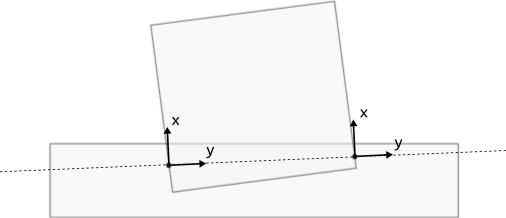
\includegraphics[clip, width=.7\hsize]{fig/phcontact.eps} \\
\end{tabular}
\end{center}
\caption{Contact configuration}
\label{fig_physics_contact}
\end{figure}

Springhead\KLUDGE で採用している接触モデルについて説明します.
\KLUDGE 第\ref{sec_physics_scene}\KLUDGE 節で述べたように,\texttt{PHSceneIf::Step}\KLUDGE によってシミュレーションを1\KLUDGE ステップ進めると,
\KLUDGE 初めに形状の交差判定と接触拘束の生成が行われます.
\KLUDGE 交差する二つの形状の交差断面と,接触拘束の関係についてFig.\,\ref{fig_physics_contact}\KLUDGE に示します.
\KLUDGE 図では簡単のために二次元で描いていますが,実際には接触断面を表す多角形の各頂点に接触拘束が作られます.
\KLUDGE 接触拘束も他の拘束と同様にソケットとプラグで構成されます.
\KLUDGE 一方で,他の拘束とは違い接触拘束は交差判定アルゴリズムによって動的に生成・破棄されます.
\KLUDGE このため,接触し合う剛体のどちらにソケットあるいはプラグが取り付けられるかは状況依存であり,外部から選択することはできません.

\KLUDGE プラグおよびソケットの向きは次のようにして決まります.
\KLUDGE まず,x\KLUDGE 軸は接触法線と平行に向きます.ただしどちらが正の向きかは状況依存です.
\KLUDGE 次に,y\KLUDGE 軸は接触点における二つの剛体の相対速度ベクトルを接触断面へ投影した向きに向きます.
\KLUDGE 最後にz\KLUDGE 軸はx\KLUDGE ,y\KLUDGE 軸に直交するように決まります.

\KLUDGE 以下では各接触拘束が課す条件について具体的に述べます.
\KLUDGE まず,法線方向の進入速度の大小に応じて衝突モデルと静的接触モデルのいずれかが選択されます.
\begin{align*}
v^\mathrm{x} < -V^\mathrm{th}   \;\; &\Rightarrow \;\; \text{\KLUDGE 衝突モデル} \\
v^\mathrm{x} \ge -V^\mathrm{th} \;\; &\Rightarrow \;\; \text{\KLUDGE 静的接触モデル}
\end{align*}
\KLUDGE ここで$v^\mathrm{x}$\KLUDGE はソケットから見たプラグの相対速度のx\KLUDGE 軸(接触法線)成分で,近づき合う向きを負とします.
\KLUDGE また,$V^\mathrm{th}$\KLUDGE は衝突モデルへ切り替わる臨界速度です.

\KLUDGE 衝突モデルでは,1\KLUDGE ステップ後の相対速度${v^\mathrm{x}}'$\KLUDGE が跳ね返り係数$e$\KLUDGE にもとづいて決まり,それを満たすような接触力が計算されます.
\begin{align}
{v^\mathrm{x}}' = - e \, v^\mathrm{x}
\end{align}
\KLUDGE ここで,跳ね返り係数は衝突する形状の物性値に定義された跳ね返り係数の平均値です.
%\KLUDGE 各形状の跳ね返り係数は,\texttt{CDShapeDesc::e}\KLUDGE か,\texttt{CDShapeIf::SetElasticity}\KLUDGE を用いて設定します
%\KLUDGE (第\ref{sec_collision_material}\KLUDGE 節参照).

\KLUDGE 静的接触モデルでは,形状同士の進入深度$d$\KLUDGE が1\KLUDGE ステップで所定の割合で減少するような接触力を求めます.
\KLUDGE つまり,1\KLUDGE ステップ後の進入深度を$d'$\KLUDGE とすると
\begin{align}
d' = d - \gamma \mathrm{max}(d - d^\mathrm{tol}, 0)
\end{align}
\KLUDGE となります.
\KLUDGE ここで$\gamma$\KLUDGE は接触拘束の誤差修正率です.
\KLUDGE また,$d^\mathrm{tol}$\KLUDGE は許容進入深度です.

\KLUDGE 最後に,接触力が満たすべき条件について述べます.
\KLUDGE まず,法線方向には反発力のみ作用することから,接触力のx\KLUDGE 軸成分$f^\mathrm{x}$\KLUDGE には
\begin{align*}
f^\mathrm{x} \ge 0
\end{align*}
\KLUDGE が課せられます.
\KLUDGE 一方で接触力のy\KLUDGE 軸成分$f^\mathrm{y}$\KLUDGE ,z\KLUDGE 軸成分$f^\mathrm{z}$\KLUDGE は摩擦力を表します.
\KLUDGE 摩擦力に関しては,その向きの相対速度にもとづき静止摩擦か動摩擦かが判定され,それに応じて最大摩擦力の制約が課されます.
\begin{align*}
-\mu_0 f^\mathrm{x} \le &f^\mathrm{y} \le \mu_0 f^\mathrm{x} & & \text{if} \; -V^\mathrm{f} \le v^\mathrm{y} \le V^\mathrm{f},\\
 \mu   f^\mathrm{x} \le &f^\mathrm{y} \le \mu   f^\mathrm{x} & & \text{otherwise}
\end{align*}
\KLUDGE ここで,静止摩擦係数$\mu_0$\KLUDGE および動摩擦係数$\mu$\KLUDGE は跳ね返り係数と同様に各形状の物性値の平均値が用いられます.
\KLUDGE また,$V^\mathrm{f}$\KLUDGE は静止摩擦と動摩擦が切り替わる臨界速度です.
z\KLUDGE 軸方向についても同様の制約が課されます.

\KLUDGE 接触モデルの関係するインタフェースには以下があります.
\begin{center}
\begin{longtable}{p{.1\hsize}p{.5\hsize}p{.4\hsize}}
\multicolumn{3}{l}{\texttt{CDShapeIf}}						\\ \midrule
\texttt{void}	& \texttt{SetElasticity(float e)}       & \KLUDGE 跳ね返り係数を設定 \\
\texttt{float}  & \texttt{GetElasticity()}              & \KLUDGE 跳ね返り係数を取得 \\
\texttt{void}   & \texttt{SetStaticFriction(float mu0)} & \KLUDGE 静摩擦係数を設定 \\
\texttt{float}  & \texttt{GetStaticFriction()}          & \KLUDGE 静摩擦係数を取得 \\
\texttt{void}   & \texttt{SetDynamicFriction(float mu)} & \KLUDGE 動摩擦係数を設定 \\
\texttt{float}  & \texttt{GetDynamicFriction()}         & \KLUDGE 動摩擦係数を取得
\end{longtable}
\end{center}

\begin{center}
\begin{longtable}{p{.1\hsize}p{.5\hsize}p{.4\hsize}}
\multicolumn{3}{l}{\texttt{PHSceneIf}}						\\ \midrule
\texttt{void}	& \texttt{SetContactTolerance(double tol)} & \KLUDGE 許容交差深度を設定 \\
\texttt{double} & \texttt{GetContactTolerance()}           & \KLUDGE 許容交差深度を取得 \\
\texttt{void}   & \texttt{SetImpactThreshold(double vth)}  & \KLUDGE 最小衝突速度を設定 \\
\texttt{double} & \texttt{GetImpactThreshold()}            & \KLUDGE 最小衝突速度を取得 \\
\texttt{void}   & \texttt{SetFrictionThreshold(double vf)} & \KLUDGE 最小動摩擦速度を設定 \\
\texttt{double} & \texttt{GetFrictionThreshold()}          & \KLUDGE 最小動摩擦速度を取得
\end{longtable}
\end{center}

\noindent\textbf{\KLUDGE 備考}
\begin{itemize}
\item \KLUDGE 接触断面の向きについては,形状同士の進入速度をもとに決定しますが,ここでは詳しく述べません.
\item \KLUDGE 摩擦力に関してはy\KLUDGE 軸,z\KLUDGE 軸が個別に扱われますが,実際の摩擦力はy\KLUDGE 成分とz\KLUDGE 成分の合力として与えられますので,
\KLUDGE 合力が最大摩擦力を超過する可能性があります.このようにSpringhead\KLUDGE の摩擦モデルはあくまで近似的なものですので
\KLUDGE 注意して下さい.
\end{itemize}

\subsection*{\KLUDGE 接触力の取得}

\KLUDGE 特定の剛体に作用する接触力を直接取得するためのインタフェースは用意されていません.
\KLUDGE このため,ユーザサイドである程度の計算を行う必要があります.
\KLUDGE 以下に,ある剛体に作用する接触力の合力を求める例を示します.

\begin{sourcecode}
// given PHSceneIf* scene
// given PHSolidIf* solid

Vec3d fsum;    //< sum of contact forces applied to "solid"
Vec3d tsum;    //< sum of contact torques applied to "solid"

int N = scene->NContacts();
Vec3d f, t;
Posed pose;

for(int i = 0; i < N; i++){
    PHContactPointIf* con = scene->GetContact(i);
    con->GetConstraintForce(f, t);

    if(con->GetSocketSolid() == solid){
        con->GetSocketPose(pose);
        fsum -= pose.Ori() * f;
        tsum -= pose.Pos() % pose.Ori() * f;
    }
    if(con->GetPlugSolid() == solid){
        con->GetPlugPose(pose);
        fsum += pose.Ori() * f;
        tsum += pose.Pos() % pose.Ori() * f;
    }
}
\end{sourcecode}
\KLUDGE まず,シーン中の接触拘束の数を\texttt{PHSceneIf::NConstacts}\KLUDGE で取得し,
\texttt{for}\KLUDGE ループ中で$i$\KLUDGE 番目の接触拘束を\texttt{PHSceneIf::GetContact}\KLUDGE で取得します.
\KLUDGE 次に\texttt{PHConstraintIf::GetConstraintForce}\KLUDGE で接触力の並進力\texttt{f}\KLUDGE とモーメント\texttt{t}\KLUDGE を取得しますが,
\KLUDGE 接触拘束の場合モーメントは$0$\KLUDGE ですので用いません.
\KLUDGE また,得られる拘束力はソケット/\KLUDGE プラグ座標系で表したもので,作用点はソケット/\KLUDGE プラグ座標系の原点です.
\KLUDGE これを考慮して剛体に作用する力とモーメントへ変換し,合力に足し合わせていきます.
\KLUDGE 剛体がソケット側である場合は作用・反作用を考慮して符号を反転することに注意して下さい.


\subsection*{\KLUDGE 接触力計算の有効/\KLUDGE 無効の切り替え}

\KLUDGE 多くのアプリケーションでは,すべての剛体の組み合わせに関して接触を取り扱う必要はありません.
\KLUDGE このような場合は必要な剛体の対に関してのみ接触を有効化することで計算コストを削減できます.
Springhead\KLUDGE では,剛体の組み合わせ毎に交差判定および接触力計算を行うかを切り替えることができます.
\KLUDGE これには\texttt{PHSceneIf::SetContactMode}\KLUDGE を用います.

\begin{center}
\begin{longtable}{p{.1\hsize}p{.9\hsize}}
\multicolumn{2}{l}{\texttt{PHSceneIf}}						\\ \midrule
\texttt{void}	& \texttt{SetContactMode(PHSolidIf* lhs, PHSolidIf* rhs, int mode)} \\
\texttt{void}   & \texttt{SetContactMode(PHSolidIf** group, size\_t length, int mode)} \\
\texttt{void}   & \texttt{SetContactMode(PHSolidIf* solid, int mode)} \\
\texttt{void}   & \texttt{SetContactMode(int mode)}
\end{longtable}
\end{center}

\KLUDGE 一番目は剛体\texttt{lhs}\KLUDGE と\texttt{rhs}\KLUDGE の対に関してモードを設定します.
\KLUDGE 二番目は配列\texttt{[group, group + length)}\KLUDGE に格納された剛体の全組み合わせに関して設定します.
\KLUDGE 三番目は剛体\texttt{solid}\KLUDGE と他の全剛体との組み合わせに関して設定します.
\KLUDGE 四番目はシーン中のすべての剛体の組み合わせに関して設定します.

\KLUDGE 設定可能なモードは以下の内の一つです.
\begin{center}
\begin{longtable}{p{.3\hsize}p{.7\hsize}}
\multicolumn{2}{l}{\texttt{PHSceneDesc::ContactMode}} \\ \midrule
\texttt{MODE\_NONE}	   & \KLUDGE 交差判定および接触力計算を行わない \\
\texttt{MODE\_LCP}     & \KLUDGE 交差判定を行い,拘束力計算法を用いる \\
\texttt{MODE\_PENALTY} & \KLUDGE 交差判定を行い,ペナルティ反力法を用いる \\
\end{longtable}
\end{center}
\KLUDGE デフォルトではすべての剛体対に関して\texttt{MODE\_LCP}\KLUDGE が選択されています.
\KLUDGE 例として,床面との接触以外をすべてオフにするには
\begin{sourcecode}
// given PHSolidIf* floor

scene->SetContactMode(PHSceneDesc::MODE_NONE);
scene->SetContactMode(floor, PHSceneDesc::MODE_LCP);
\end{sourcecode}
\KLUDGE とします.

\section{\KLUDGE 関節座標系シミュレーション}

\index{\KLUDGE かんせつざひょうけい@\KLUDGE 関節座標系}
T.B.D.


\section{\KLUDGE ギア}

\index{\KLUDGE ぎあ@\KLUDGE ギア}
T.B.D.

\section{\KLUDGE 内部アルゴリズムの設定}
\label{sec_physics_engine}

\KLUDGE 以下では物理シミュレーションの内部で用いられているアルゴリズムの詳細な設定項目について説明します.

\subsection*{\KLUDGE 拘束力計算エンジン}

\KLUDGE 拘束力計算エンジンは,関節や接触などの拘束を満足するための拘束力の計算を行います.
\KLUDGE 拘束力計算エンジンのクラスは\texttt{PHConstraintEngineIf}\KLUDGE で,これを取得するには以下の関数を用います.


\texttt{PHConstraintEngineIf}\KLUDGE のインタフェースを以下に示します.

\begin{center}
\begin{longtable}{p{.12\hsize}p{.45\hsize}p{.33\hsize}}
\multicolumn{3}{l}{\texttt{PHConstraintEngineIf}}			\\ \midrule
\texttt{void}	& \texttt{SetVelCorrectionRate(double)}		& \KLUDGE 関節拘束の誤差修正率を設定 \\
\texttt{double} & \texttt{GetVelCorrectionRate()}			& \KLUDGE 関節拘束の誤差修正率を取得 \\
\texttt{void}	& \texttt{SetContactCorrectionRate(double)}	& \KLUDGE 接触拘束の誤差修正率を設定 \\
\texttt{double} & \texttt{GetContactCorrectionRate()}		& \KLUDGE 接触拘束の誤差修正率を取得 \\
\end{longtable}
\end{center}

\KLUDGE 誤差修正率とは,1\KLUDGE ステップで拘束誤差どの程度修正するかを示す比率で,通常$[0, 1]$\KLUDGE の値を設定します.
\KLUDGE 誤差修正率を$1$\KLUDGE にすると,1\KLUDGE ステップで拘束誤差を$0$\KLUDGE にするような拘束力が計算されますが,発振現象などのシミュレーションの不安定化を招く傾向があります.
\KLUDGE 逆に修正率を小さ目に設定すればシミュレーションは安定化しますが,定常誤差が増大します.

\KLUDGE 拘束力計算エンジンは,内部で反復型のアルゴリズムで拘束力を計算します.
\KLUDGE アルゴリズムの反復回数は\texttt{PHSceneIf::SetNumIteration}\KLUDGE で設定します(第\ref{sec_physics_scene}\KLUDGE 節参照).


\texttt{PHSceneIf::SetContactTolerance}\KLUDGE で設定可能です.

\texttt{PHConstraintEngineIf::SetContactCorrectionRate}\KLUDGE で設定可能です
\KLUDGE (第\ref{sec_physics_engine}\KLUDGE 節参照).


\chapter{Graphics}
\label{chap_graphics}
\section{\KLUDGE 概要}

\index{Graphics}
Graphics\KLUDGE は3D\KLUDGE シーンの描画機能を提供するモジュールです.

\section{Graphics SDK}

\index{GRSdk}
Graphics\KLUDGE モジュールのすべてのオブジェクトはSDK\KLUDGE クラス\texttt{GRSdk}\KLUDGE によって管理されます.
\texttt{GRSdk}\KLUDGE クラスは,プログラムの実行を通してただ1つのオブジェクトが存在するシングルトンクラスです.
\texttt{GRSdk}\KLUDGE オブジェクトを作成するには以下のようにします.
\begin{verbatim}
    GRSdkIf* grSdk = GRSdkIf::CreateSdk();
\end{verbatim}
\KLUDGE 通常この操作はプログラムの初期化時に一度だけ実行します.
\KLUDGE また,Framework\KLUDGE モジュールを使用する場合はユーザが直接\texttt{GRSdk}\KLUDGE を作成する必要はありません.

\texttt{GRSdk}\KLUDGE には以下の機能があります.
\begin{itemize}
\item \KLUDGE レンダラの作成
\item \KLUDGE デバイスの作成
\item \KLUDGE シーンの管理
\end{itemize}

\index{GRRender}
\index{\KLUDGE レンダラ}
\KLUDGE レンダラとは処理系に依存しない抽象化された描画機能を提供するクラスです.
\KLUDGE レンダラのクラスは\texttt{GRRender}\KLUDGE です.

\index{GRDeviceGL}
\index{\KLUDGE デバイス}
\KLUDGE 一方,デバイスは処理系ごとの描画処理の実装を行うクラスです.
\KLUDGE 現在のSpringhead\KLUDGE ではOpenGL\KLUDGE による描画のみがサポートされています.
OpenGL\KLUDGE 用デバイスクラスは\texttt{GRDeviceGL}\KLUDGE です.

\KLUDGE レンダラをデバイスに関する\texttt{GRSdk}\KLUDGE の関数を以下に示します.

\begin{center}
\begin{tabular}{p{.2\hsize}p{.40\hsize}p{.3\hsize}}
\texttt{GRSdkIf}		&								&	\\ \midrule
\texttt{GRRenderIf*} 	& \texttt{CreateRender()}		& \KLUDGE レンダラを作成		\\
\texttt{GRDeviceGLIf*} 	& \texttt{CreateDeviceGL()}		& OpenGL\KLUDGE デバイスを作成	\\
\end{tabular}
\end{center}

\begin{center}
\begin{tabular}{p{.2\hsize}p{.40\hsize}p{.3\hsize}}
\texttt{GRRenderIf}		&									&	\\ \midrule
\texttt{void}			& \texttt{SetDevice(GRDeviceIf*)}	& \KLUDGE デバイスの設定	\\
\texttt{GRDeviceIf*} 	& \texttt{GetDevice()}				& \KLUDGE デバイスの取得	\\
\end{tabular}
\end{center}

\subsection*{\KLUDGE 初期化}

Graphics\KLUDGE モジュールを使用するには以下の初期化処理を必ず実行する必要があります.
\begin{verbatim}
   	GRRenderIf* render = grSdk->CreateRender();
    GRDeviceIf* device = grSdk->CreateDeviceGL();
    device->Init();
    render->SetDevice(device);
\end{verbatim}
\texttt{GRRender}\KLUDGE の\texttt{SetDevice}\KLUDGE 関数でデバイスを登録すると,レンダラは実際の描画処理をそのデバイスを用いて行います.
\KLUDGE 将来的に処理系ごとにデバイスを使い分けることを想定し,上の処理はユーザが行うことになっています.
Framework\KLUDGE モジュールを使用する場合はユーザ自身で上の手続きを行う必要はありません.

\section{\KLUDGE シーン}
\label{sec_grscene}

\subsection*{\KLUDGE シーンの作成}

\index{GRScene}
Graphics\KLUDGE モジュールのシーンは,コンピュータグラフィクスにおけるいわゆるシーングラフと同等のものです.
\KLUDGE シーンクラスは\texttt{GRScene}\KLUDGE です.
\KLUDGE シーンを作成するには次のようにします.
\begin{verbatim}
    GRSceneIf* grScene = grSdk->CreateScene();
\end{verbatim}
\texttt{GRScene}\KLUDGE はディスクリプタによる設定項目を持ちません.
\KLUDGE また,Fig.\,\ref{fig_grscene}\KLUDGE に示すように\texttt{GRSdk}\KLUDGE オブジェクトは任意の数のシーンを保持できます.

\KLUDGE シーン作成に関する\texttt{GRSdk}\KLUDGE の関数は以下の通りです.

\begin{center}
\begin{tabular}{p{.15\hsize}p{.50\hsize}p{.25\hsize}}
\texttt{GRSdkIf}	&												&	\\ \midrule
\texttt{GRSceneIf*}	& \texttt{CreateScene()}						& \KLUDGE シーンを作成			\\
\texttt{GRSceneIf*}	& \texttt{GetScene(size\_t)}					& \KLUDGE シーンを取得			\\
\texttt{size\_t}	& \texttt{NScene()}								& \KLUDGE シーンの数			\\
\texttt{void}		& \texttt{MergeScene(GRSceneIf*, GRSceneIf*)}	& \KLUDGE シーンの統合			\\
\end{tabular}
\end{center}

\begin{figure}[t]
\begin{center}
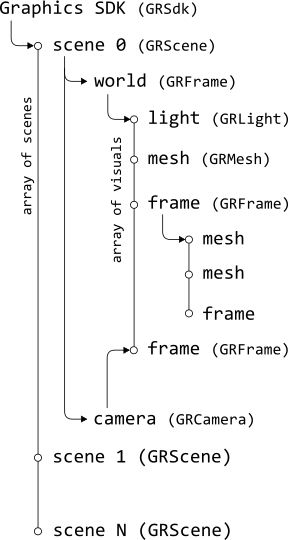
\includegraphics[width=.4\hsize]{fig/grscene.eps}
\end{center}
\caption{Graphics data structure}
\label{fig_grscene}
\end{figure}

\subsection*{\KLUDGE シーンの機能}

\KLUDGE シーンを作成したら,次はそのコンテンツであるフレームやメッシュ,カメラやライトなどを作成してシーンに加えていきます.
\KLUDGE この方法としては完全に手動でシーンを構築する他にもFileIO\KLUDGE モジュールを使用してファイルからシーンをロードする方法もあります.
\KLUDGE 以下に\texttt{GRScene}\KLUDGE の関数を示します.

\begin{center}
\begin{tabular}{p{.15\hsize}p{.45\hsize}p{.3\hsize}}
\texttt{GRSceneIf}	 &															&	\\ \midrule
\texttt{GRFrameIf*}	 & \texttt{GetWorld()}										& \KLUDGE ワールドフレームの取得	\\
\texttt{GRCameraIf*} & \texttt{GetCamera()}										& \KLUDGE カメラの取得	\\
\texttt{void}		 & \texttt{SetCamera(const GRCameraDesc\&)}					& \KLUDGE カメラの設定	\\
\texttt{GRVisualIf*} & \texttt{CreateVisual(const GRVisualDesc\&, GRFrameIf*)}	& \KLUDGE 描画アイテムの作成	\\
\texttt{void}		 & \texttt{Render(GRRenderIf*)}								& \KLUDGE 描画	\\
\end{tabular}
\end{center}

%	///	\KLUDGE アニメーションコントローラの取得
%	GRAnimationControllerIf* GetAnimationController();

Fig.\,\ref{fig_grscene}\KLUDGE に示すように,1\KLUDGE つのシーンはただ1\KLUDGE つのワールドフレームを持ち,それを基点として
\KLUDGE 任意の数の描画アイテムがツリー状に連なります.
\KLUDGE ワールドフレームは\texttt{GetWorld}\KLUDGE で取得します.

\KLUDGE 特殊な描画アイテムにカメラがあります.
\KLUDGE カメラはワールドフレーム以下のツリーとは別に,\texttt{GRScene}\KLUDGE が保持します(Fig.\,\ref{fig_grscene})\KLUDGE .
\KLUDGE カメラの設定は\texttt{SetCamera}\KLUDGE で行います.
\KLUDGE カメラを取得するには\texttt{GetCamera}\KLUDGE を使います.
\KLUDGE また,カメラはシーングラフ中の1\KLUDGE つのフレームを参照し,これを視点の設定に用います.
\KLUDGE イメージとしてはカメラが参照先のフレームに取り付けられていると考える方が自然でしょう.
\KLUDGE 参照先のフレームの移動に応じてカメラもシーン中を移動することになります.


\subsection*{\KLUDGE シーンの描画}

\KLUDGE 描画処理はプログラムの描画ハンドラで行います.GLUT\KLUDGE を使う場合は\texttt{glutDisplayFunc}\KLUDGE で登録したコールバック関数がこれにあたり,
\KLUDGE またFramework\KLUDGE モジュールの\texttt{FWApp}\KLUDGE を使う場合は\texttt{Display}\KLUDGE 仮想関数がこれにあたります.
\KLUDGE 以下が典型的な描画処理です.
\begin{verbatim}
    render->ClearBuffer();        // clear back buffer
    render->BeginScene();         // begin rendering

    grScene->Render(render);      // render scene

    render->EndScene();           // end rendering
    render->SwapBuffers();        // swap buffers
\end{verbatim}

\texttt{ClearBuffer}\KLUDGE は描画バッファを所定の色で塗りつぶします.
\KLUDGE 塗りつぶし色の取得/\KLUDGE 設定は\texttt{GRRender}\KLUDGE の\texttt{GetClearColor}\KLUDGE ,\text{SetClearColor}\KLUDGE を使います.
\begin{verbatim}
    render->SetClearColor(Vec4f(1.0f, 0.0f, 0.0f, 1.0f));
    render->ClearBuffer();        // clear back buffer in red
\end{verbatim}

\texttt{BeginScene}\KLUDGE と\texttt{EndScene}\KLUDGE はシーンの描画の前後で必ず呼び出します.
\texttt{SwapBuffers}\KLUDGE はフロントバッファとバックバッファを切り換えることで描画内容を画面上に表示します.

\texttt{GRScene}\KLUDGE の\texttt{Render}\KLUDGE 関数は,カメラ(\texttt{GRCamera})\KLUDGE の\texttt{Render}\KLUDGE とワールドフレーム(\texttt{GRFrame})\KLUDGE の\texttt{Render}\KLUDGE を
\KLUDGE 順次呼び出します.まずカメラの描画によって視点と投影変換が設定され,
\KLUDGE 次にワールドフレームの描画によってシーングラフが再帰的に描画されます.

\section{\KLUDGE 描画アイテム}

\begin{figure}[t]
\begin{center}
\includegraphics[width=.4\hsize]{fig/grvisual.eps}
\end{center}
\caption{Class hierarchy of visual items}
\label{fig_grvisual}
\end{figure}

\index{GRVisual}
\KLUDGE シーングラフを構成する描画アイテムの基本クラスは\texttt{GRVisual}\KLUDGE です.
\texttt{GRVisual}\KLUDGE から派生するクラスをFig.\,\ref{fig_grvisual}\KLUDGE に示します.
\KLUDGE 描画アイテムには以下の共通の機能があります.

\begin{center}
\begin{tabular}{p{.15\hsize}p{.45\hsize}p{.3\hsize}}
\multicolumn{3}{l}{\texttt{GRVisualIf}}					\\ \midrule
\texttt{void}	& \texttt{Render(GRRenderIf*)}		& 	\\
\texttt{void} 	& \texttt{Rendered(GRRenderIf*)}	& 	\\
\texttt{void} 	& \texttt{Enable(bool)}				& 	\\
\texttt{bool} 	& \texttt{IsEnabled()}				& 	\\
\end{tabular}
\end{center}

\texttt{Render}\KLUDGE はアイテムの描画を行い,\texttt{Rendered}\KLUDGE は描画の後処理を行います.
\KLUDGE 描画処理は描画アイテムの種類ごとに異なります.
\KLUDGE これについては次節以降で説明します.

\texttt{Enable}\KLUDGE 関数は描画処理の有効化/\KLUDGE 無効化を行います.
\KLUDGE 無効化されたアイテムは描画されません.
\texttt{IsEnabled}\KLUDGE 関数は有効/\KLUDGE 無効状態を返します.

\KLUDGE 描画アイテムを作成するには\texttt{GRScene}\KLUDGE の\texttt{CreateVisual}\KLUDGE 関数に種類ごとのディスクリプタを指定して呼び出します.


\section{\KLUDGE フレーム}

\index{GRFrame}
\index{\KLUDGE ふれーむ@\KLUDGE フレーム}
\KLUDGE フレームは座標変換を定義すると同時に他の描画アイテムのコンテナとしての役割を持ちます.
\KLUDGE フレームのクラスは\texttt{GRFrame}\KLUDGE です.
\KLUDGE 次のコードは,フレームを作成してワールドフレームの子として登録します.
\begin{verbatim}
    GRFrameDesc desc;
    GRFrameIf* frame =
        grScene->CreateVisual(desc, grScene->GetWorldFrame())->Cast();
\end{verbatim}
\texttt{CreateVisual}\KLUDGE 関数は指定されたディスクリプタに対応する描画アイテムを作成し,
\KLUDGE 指定された親フレームの子として登録します.親フレームを省くとデフォルトでワールドフレームに登録されます.
\KLUDGE したがって上のコードは\texttt{CreateVisual(desc)}\KLUDGE としてもかまいません.

\texttt{GRFrame}\KLUDGE の\texttt{Render}\KLUDGE 関数は,子描画アイテムの\texttt{Render}\KLUDGE を順次呼び出します.


\subsection*{\KLUDGE 親子関係}

\KLUDGE フレーム間の親子関係を管理する関数には次のものがあります.

\begin{center}
\begin{tabular}{p{.20\hsize}p{.45\hsize}p{.25\hsize}}
\multicolumn{3}{l}{\texttt{GRFrameIf}}						\\ \midrule
\texttt{GRFrameIf*}		& \texttt{GetParent()}				& 	\\
\texttt{void} 			& \texttt{SetParent(GRFrameIf*)}	& 	\\
\texttt{int} 			& \texttt{NChildren()}				& 	\\
\texttt{GRVisualIf**} 	& \texttt{GetChildren()}			& 	\\
\end{tabular}
\end{center}

\texttt{GetParent}\KLUDGE は親フレームを取得します.
\texttt{SetParent}\KLUDGE はそのフレームの親フレームを変更するために使います.
\texttt{NChildren}\KLUDGE はそのフレームの子である描画アイテムの数を返します.
\KLUDGE これらにはフレーム以外の描画アイテムも含まれることに注意してください.
\texttt{GetChildren}\KLUDGE は子描画アイテムの配列を取得します.


\subsection*{\KLUDGE 座標変換}

\KLUDGE フレームの座標変換を操作する関数は以下の通りです.

\begin{center}
\begin{tabular}{p{.15\hsize}p{.45\hsize}p{.3\hsize}}
\multicolumn{3}{l}{\texttt{GRFrameIf}}							\\ \midrule
\texttt{Affinef} & \texttt{GetTransform()}					& 	\\
\texttt{Affinef} & \texttt{GetWorldTransform()}				& 	\\
\texttt{void}	 & \texttt{SetTransform(const Affinef\&)}	& 	\\
\end{tabular}
\end{center}

\texttt{GetTransform}\KLUDGE ,\texttt{SetTransform}\KLUDGE はそれぞれフレームとその親フレームとの間の相対的な座標変換を取得/\KLUDGE 設定します.
\KLUDGE 例えば
\begin{verbatim}
    frame->SetTransform(Affinef::Trn(1.0, 0.0, 0.0));
\end{verbatim}
\KLUDGE とすると親フレームに対して相対的にx\KLUDGE 方向に$1.0$\KLUDGE 移動します.

\section{\KLUDGE カメラ}

\begin{figure}[t]
\begin{tabular}{c}
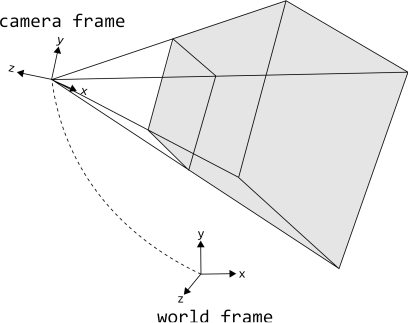
\includegraphics[width=.4\hsize]{fig/grcamera.eps} \\
(a) Perspective frustum \\
\\
\begin{tabular}{cc}
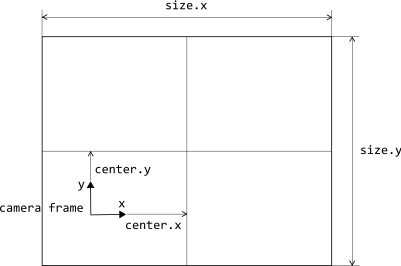
\includegraphics[width=.4\hsize]{fig/grcamera_front.eps} &
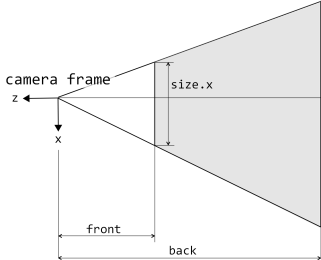
\includegraphics[width=.4\hsize]{fig/grcamera_top.eps} \\
(b) Front view of screen &
(c) Top view of screen
\end{tabular}
\end{tabular}
\caption{Camera parameters}
\label{fig_grcamera}
\end{figure}

\index{GRCamera}
\index{\KLUDGE かめら@\KLUDGE カメラ}
\KLUDGE カメラは描画における視点の設定と投影変換を管理します.
\KLUDGE はじめにカメラのディスクリプタを見ていきます.

\begin{center}
\begin{tabular}{p{.15\hsize}p{.45\hsize}p{.3\hsize}}
\multicolumn{3}{l}{\texttt{GRCameraDesc}}					\\ \midrule
\texttt{Vec2f}	&	\texttt{size}	& \KLUDGE スクリーンサイズ 		\\
\texttt{Vec2f}	&	\texttt{center}	& \KLUDGE スクリーン中心座標 	\\
\texttt{float}	&	\texttt{front}	& \KLUDGE 前方クリップ面		\\
\texttt{float}	&	\texttt{back}	& \KLUDGE 後方クリップ面		\\
\end{tabular}
\end{center}

\KLUDGE 各変数の定義はFig.\,\ref{fig_grcamera}(b),(c)\KLUDGE を参照してください.
\KLUDGE 設定を変更するには以下のようにします.
\begin{verbatim}
    GRCameraDesc desc;
    grScene->GetCamera()->GetDesc(&desc);
    desc.front = 3.0f;
    grScene->SetCamera(desc);
\end{verbatim}
\KLUDGE 上では\texttt{GetDesc}\KLUDGE 関数で既存の設定をディスクリプタにコピーし,\texttt{front}\KLUDGE を変更してから
\texttt{SetCamera}\KLUDGE 関数で再設定しています.

\KLUDGE 一方,\texttt{GRCamera}\KLUDGE の関数は以下の通りです.

\begin{center}
\begin{tabular}{p{.15\hsize}p{.45\hsize}p{.3\hsize}}
\multicolumn{3}{l}{\texttt{GRCameraIf}}					\\ \midrule
\texttt{GRFrameIf*}	& \texttt{GetFrame()}				&	\\
\texttt{void}		& \texttt{SetFrame(GRFrameIf*)}		&	\\
\end{tabular}
\end{center}

\texttt{GetFrame}\KLUDGE ,\texttt{SetFrame}\KLUDGE 関数はカメラフレームを取得/\KLUDGE 設定します.
Fig.\,\ref{fig_grcamera}(a)\KLUDGE のように,カメラフレームはカメラの視点を定義します.

\section{\KLUDGE ライト}

\index{GRLight}
\index{\KLUDGE らいと@\KLUDGE ライト}
\KLUDGE ライトはシーンの照明を設定するための描画アイテムです.
\KLUDGE ライトのクラス\texttt{GRLight}\KLUDGE のディスクリプタの代表的な変数を以下に示します.

\begin{center}
\begin{tabular}{p{.15\hsize}p{.45\hsize}p{.3\hsize}}
\multicolumn{3}{l}{\texttt{GRLightDesc}}				\\ \midrule
\texttt{Vec4f}	&	\texttt{ambient}	& \KLUDGE 環境光 		\\
\texttt{Vec4f}	&	\texttt{diffuse}	& \KLUDGE 拡散光 		\\
\texttt{Vec4f}	&	\texttt{specular}	& \KLUDGE 鏡面光		\\
\texttt{Vec4f}	&	\texttt{position}	& \KLUDGE ライト位置	\\
\end{tabular}
\end{center}

\KLUDGE 減衰係数やスポットライトなどのより詳細な設定項目についてはソースファイルを参照してください.
OpenGL\KLUDGE の仕様と同様,\texttt{position}\KLUDGE の第4\KLUDGE 成分\texttt{position.w}\KLUDGE が$0$\KLUDGE の場合は平行光源となり,
\texttt{(x,y,z)}\KLUDGE 方向の無限遠にライトがあることになり,\texttt{position.w}\KLUDGE が$1$\KLUDGE の場合は
\texttt{(x,y,z)}\KLUDGE の位置に点光源がおかれます.

\section{\KLUDGE マテリアル}
\label{sec_grmaterial}

\index{GRMaterial}
\index{\KLUDGE まてりある@\KLUDGE マテリアル}
\KLUDGE マテリアルは材質を指定するためのアイテムです.
\KLUDGE マテリアルのクラスは\texttt{GRMaterial}\KLUDGE です.
\KLUDGE 通常,マテリアルは次節で説明するメッシュの子描画アイテムとなります.
\KLUDGE ファイルからメッシュをロードする場合は,メッシュの作成と同時にマテリアルも自動的に作成され,メッシュの子として追加されます.
\texttt{GRMaterial}\KLUDGE のディスクリプタは以下の通りです.

\begin{center}
\begin{tabular}{p{.15\hsize}p{.45\hsize}p{.3\hsize}}
\multicolumn{3}{l}{\texttt{GRMaterialDesc}}				\\ \midrule
\texttt{Vec4f}		&	\texttt{ambient}	& \KLUDGE 環境色 	\\
\texttt{Vec4f}		&	\texttt{diffuse}	& \KLUDGE 拡散色 	\\
\texttt{Vec4f}		&	\texttt{specular}	& \KLUDGE 鏡面色	\\
\texttt{Vec4f}		&	\texttt{emissive}	& \KLUDGE 自己発光	\\
\texttt{float}		&	\texttt{power}		& \KLUDGE 鏡面係数	\\
\texttt{UTString}	&	\texttt{texname}	& \KLUDGE テクスチャファイル名
\end{tabular}
\end{center}

\KLUDGE レンダラにマテリアルを設定すると,次に別のマテリアルを設定するまでの間の
\KLUDGE 形状描画にそのマテリアルの描画属性が適用されます.
\KLUDGE マテリアルを設定するにはいくつかの方法があります.
\KLUDGE 一つ目は\texttt{GRMaterialIf}\KLUDGE の\texttt{Render}\KLUDGE 関数を呼ぶ方法です:
\KLUDGE これに加え,以下に示す\texttt{GRRender}\KLUDGE の関数のいずれかを用いることもできます.
\begin{center}
\begin{tabular}{p{.1\hsize}p{.5\hsize}p{.3\hsize}}
\texttt{GRRenderIf}																\\ \midrule
\texttt{void} & \texttt{SetMaterial(const GRMaterialDesc\&)}		& \KLUDGE 描画マテリアルの設定	\\
\texttt{void} & \texttt{SetMaterial(const GRMaterialIf*)}			& \KLUDGE 描画マテリアルの設定	\\
\texttt{void} & \texttt{SetMaterial(int)}							& \KLUDGE 描画マテリアルの設定	\\
\end{tabular}
\end{center}
\KLUDGE 以下の例はマテリアルを設定する3\KLUDGE 通りの方法を示しています.
\KLUDGE どの方法を用いても結果は変わりません.
\begin{verbatim}
    // given GRRenderIf* render, GRSceneIf* scene
    GRMaterialDesc md;
    md.diffuse = Vec4f(1.0f, 0.0f, 0.0f, 1.0f);
    // 1.
    render->SetMaterial(md);
    // 2.
    GRMaterialIf* mat = scene->CreateVisual(md)->Cast();
    mat->Render(render);
    // 3.
    render->SetMaterial(mat);
\end{verbatim}
\KLUDGE 毎回マテリアルを作成するのは煩わしいことがあります.
\KLUDGE そのような場合はレンダラの予約色を指定することも可能です.
\begin{verbatim}
    // 4.
    render->SetMaterial(GRRenderBaseIf::RED);
\end{verbatim}
\KLUDGE 使用可能な予約色はX11 web color\KLUDGE にもとづいています.
\KLUDGE 詳しくは\texttt{SprGRRender.h}\KLUDGE ヘッダファイルを

%%%%%%%%%%%%%%%%%%%%%%%%%%%%%%%%%%%%%%%%%%%%%%%%%%%%%%%%%%%%%%%%%%%%%%%%%%%%%%%%%%%%%%
\begin{comment}

\begin{table}[t]
\caption{Reserved colors}
\label{table_material_sample}
{\small
\begin{center}
\begin{tabular}{ll|ll}
RED				& {\color[RGB]{255,0,0}$\blacksquare$} 			(1.00, 0.00, 0.00)	&
GREEN			& {\color[rgb]{0,1,0}$\blacksquare$} 			(0.00, 1.00, 0.00)	\\
BLUE			& {\color[rgb]{0,0,1}$\blacksquare$} 			(0.00, 0.00, 1.00)	&
YELLOW			& {\color[rgb]{1,1,0}$\blacksquare$} 			(1.00, 1.00, 0.00)	\\
CYAN			& {\color[rgb]{0,1,1}$\blacksquare$} 			(0.00, 1.00, 1.00)	&
MAGENTA			& {\color[rgb]{1,0,1}$\blacksquare$} 			(1.00, 0.00, 1.00)	\\
WHITE			& {$\square$} 						 			(1.00, 1.00, 1.00)	&
GRAY			& {\color[rgb]{.5,.5,.5}$\blacksquare$} 		(0.50, 0.50, 0.50)	\\
ORANGE			& {\color[rgb]{1,.27,0}$\blacksquare$} 			(1.00, 0.27, 0.00)	&
BROWN			& {\color[rgb]{.198,0,0}$\blacksquare$} 		(0.19, 0.00, 0.00)	\\
LIGHT\_BLUE		& {\color[rgb]{.676,.844,.898}$\blacksquare$} 	(0.67, 0.84, 0.89)	&
MEDIUM\_PURPLE	& {\color[rgb]{.574,.438,.855}$\blacksquare$} 	(0.57, 0.43, 0.85)	\\
DARK\_GREEN		& {\color[rgb]{0,.391,0}$\blacksquare$} 		(0.00, 0.39, 0.00)	&
DARK\_VIOLET	& {\color[rgb]{.578,0,.824}$\blacksquare$} 		(0.57, 0.00, 0.82)	\\
DARK\_CYAN		& {\color[rgb]{0,.543,.543}$\blacksquare$} 		(0.00, 0.54, 0.54)	&
GREEN\_YELLOW	& {\color[rgb]{.676,1,.184}$\blacksquare$} 		(0.67, 1.00, 0.18)	\\
LIME\_GREEN		& {\color[rgb]{.195,.801,.195}$\blacksquare$} 	(0.19, 0.80, 0.19)	&
INDIAN\_RED		& {\color[rgb]{.801,.359,.359}$\blacksquare$} 	(0.80, 0.35, 0.35)	\\
INDIGO			& {\color[rgb]{.293,0,.508}$\blacksquare$} 		(0.29, 0.00, 0.50)	&
GREEN\_INDIGO	& {\color[rgb]{0,.198,.198}$\blacksquare$} 		(0.00, 0.19, 0.19)	\\
OLIVE\_GREEN	& {\color[rgb]{.198,.398,0}$\blacksquare$} 		(0.19, 0.39, 0.00)	&
NAVY\_BLUE		& {\color[rgb]{.198,.398,.797}$\blacksquare$} 	(0.19, 0.39, 0.79)	\\
TURQUOISE\_BLUE	& {\color[rgb]{.398,1,.797}$\blacksquare$} 		(0.39, 1.00, 0.79)	&
EMERALD\_GREEN	& {\color[rgb]{.598,1,.398}$\blacksquare$} 		(0.59, 1.00, 0.39)
\end{tabular}
\end{center}
}
\end{table}

\end{comment}
%%%%%%%%%%%%%%%%%%%%%%%%%%%%%%%%%%%%%%%%%%%%%%%%%%%%%%%%%%%%%%%%%%%%%%%%%%%%%%%%%%%%%%

\begin{table}[t]
\caption{Reserved colors}
\label{table_material_sample}
{\tiny
\begin{center}
\ifLwarp\else
\begin{tabular}{l|l}
\fi
\begin{tabular}{lll}
INDIANRED		& {\color[RGB]{205,92,92}$\blacksquare$}	& (205 92 92) \\
LIGHTCORAL		& {\color[RGB]{240,128,128}$\blacksquare$}	& (240 128 128) \\
SALMON			& {\color[RGB]{250,128,114}$\blacksquare$}	& (250 128 114) \\
DARKSALMON		& {\color[RGB]{233,150,122}$\blacksquare$}	& (233 150 122) \\
LIGHTSALMON		& {\color[RGB]{255,160,122}$\blacksquare$}	& (255 160 122) \\
RED				& {\color[RGB]{255,0,0}$\blacksquare$}		& (255 0 0) \\
CRIMSON			& {\color[RGB]{220,20,60}$\blacksquare$}	& (220 20 60) \\
FIREBRICK		& {\color[RGB]{178,34,34}$\blacksquare$}	& (178 34 34) \\
DARKRED			& {\color[RGB]{139,0,0}$\blacksquare$}		& (139 0 0) \\
\\
PINK			& {\color[RGB]{255,192,203}$\blacksquare$}	& (255 192 203)	\\
LIGHTPINK		& {\color[RGB]{255,182,193}$\blacksquare$}	& (255 182 193)	\\
HOTPINK			& {\color[RGB]{255,105,180}$\blacksquare$}	& (255 105 180)	\\
DEEPPINK		& {\color[RGB]{255, 20,147}$\blacksquare$}	& (255  20 147)	\\
MEDIUMVIOLETRED	& {\color[RGB]{199, 21,133}$\blacksquare$}	& (255  21 133)	\\
PALEVIOLETRED	& {\color[RGB]{219,112,147}$\blacksquare$}	& (255 112 147)	\\
\\
CORAL			& {\color[RGB]{255,127, 80}$\blacksquare$}	& (255 127 80)	\\
TOMATO			& {\color[RGB]{255, 99, 71}$\blacksquare$}	& (255  99 71)	\\
ORANGERED		& {\color[RGB]{255, 69,  0}$\blacksquare$}	& (255  69 0)	\\
DARKORANGE		& {\color[RGB]{255,140,  0}$\blacksquare$}	& (255 140 0)	\\
ORANGE			& {\color[RGB]{255,165,  0}$\blacksquare$}	& (255 165 0)	\\
\\
GOLD					& {\color[RGB]{255,215,0}$\blacksquare$}	& (255 215 0)	\\
YELLOW					& {\color[RGB]{255,255,0}$\blacksquare$}	& (255 255 0)	\\
LIGHTYELLOW				& {\color[RGB]{255,255,224}$\blacksquare$}	& (255 255 224)	\\
LEMONCHIFFON			& {\color[RGB]{255,250,205}$\blacksquare$}	& (255 250 205)	\\
LIGHTGOLDENRODYELLOW	& {\color[RGB]{250,250,210}$\blacksquare$}	& (250 250 210)	\\
PAPAYAWHIP				& {\color[RGB]{255,239,213}$\blacksquare$}	& (255 239 213)	\\
MOCCASIN				& {\color[RGB]{255,228,181}$\blacksquare$}	& (255 228 181)	\\
PEACHPUFF				& {\color[RGB]{255,218,185}$\blacksquare$}	& (255 218 185)	\\
PALEGOLDENROD			& {\color[RGB]{238,232,170}$\blacksquare$}	& (238 232 170)	\\
KHAKI					& {\color[RGB]{240,230,140}$\blacksquare$}	& (240 230 140)	\\
DARKKHAKI				& {\color[RGB]{189,183,107}$\blacksquare$}	& (189 183 107)	\\
\\						
LAVENDAR				& {\color[RGB]{230,230,250}$\blacksquare$}	& (230 230 250)	\\
THISTLE					& {\color[RGB]{216,191,216}$\blacksquare$}	& (216 191 216)	\\
PLUM					& {\color[RGB]{221,160,221}$\blacksquare$}	& (221 160 221)	\\
VIOLET					& {\color[RGB]{238,130,238}$\blacksquare$}	& (238 130 238)	\\
ORCHILD					& {\color[RGB]{218,112,214}$\blacksquare$}	& (218 112 214)	\\
FUCHSIA					& {\color[RGB]{255,0,255}$\blacksquare$}	& (255 0 255)	\\
MAGENTA					& {\color[RGB]{255,0,255}$\blacksquare$}	& (255 0 255)	\\
MEDIUMORCHILD			& {\color[RGB]{186,85,211}$\blacksquare$}	& (186 85 211)	\\
MEDIUMPURPLE			& {\color[RGB]{147,112,219}$\blacksquare$}	& (147 112 219)	\\
BLUEVIOLET				& {\color[RGB]{138,43,226}$\blacksquare$}	& (138 43 226)	\\
DARKVIOLET				& {\color[RGB]{148,0,211}$\blacksquare$}	& (148 0 211)	\\
DARKORCHILD				& {\color[RGB]{153,50,204}$\blacksquare$}	& (153 50 204)	\\
DARKMAGENTA				& {\color[RGB]{139,0,139}$\blacksquare$}	& (139 0 139)	\\
PURPLE					& {\color[RGB]{128,0,128}$\blacksquare$}	& (128 0 128)	\\
INDIGO					& {\color[RGB]{75,0,130}$\blacksquare$}	& (75 0 130)	\\
DARKSLATEBLUE			& {\color[RGB]{72,61,139}$\blacksquare$}	& (72 61 139)	\\
SLATEBLUE				& {\color[RGB]{106,90,205}$\blacksquare$}	& (106 90 205)	\\
MEDIUMSLATEBLUE			& {\color[RGB]{123,104,238}$\blacksquare$}	& (123 104 238)	\\
\\
GREENYELLOW				& {\color[RGB]{173,255,47}$\blacksquare$}	& (173 255 47)	\\
CHARTREUSE				& {\color[RGB]{127,255,0}$\blacksquare$}	& (127 255 0)	\\
LAWNGREEN				& {\color[RGB]{124,252,0}$\blacksquare$}	& (124 252 0)	\\
LIME					& {\color[RGB]{0,255,0}$\blacksquare$}	& (0 255 0)	\\
LIMEGREEN				& {\color[RGB]{50,205,50}$\blacksquare$}	& (50 205 50)	\\
PALEGREEN				& {\color[RGB]{152,251,152}$\blacksquare$}	& (152 251 152)	\\
LIGHTGREEN				& {\color[RGB]{144,238,144}$\blacksquare$}	& (144 238 144)	\\
MEDIUMSPRINGGREEN		& {\color[RGB]{0,250,154}$\blacksquare$}	& (0 250 154)	\\
SPRINGGREEN				& {\color[RGB]{0,255,127}$\blacksquare$}	& (0 255 127)	\\
MEDIUMSEAGREEN			& {\color[RGB]{60,179,113}$\blacksquare$}	& (60 179 113)	\\
SEAGREEN				& {\color[RGB]{46,139,87}$\blacksquare$}	& (46 139 87)	\\
FORESTGREEN				& {\color[RGB]{34,139,34}$\blacksquare$}	& (34 139 34)	\\
GREEN					& {\color[RGB]{0,128,0}$\blacksquare$}	& (0 128 0)	\\
DARKGREEN				& {\color[RGB]{0,100,0}$\blacksquare$}	& (0 100 0)	\\
YELLOWGREEN				& {\color[RGB]{154,205,50}$\blacksquare$}	& (154 205 50)	\\
OLIVEDRAB				& {\color[RGB]{107,142,35}$\blacksquare$}	& (107 142 35)	\\
OLIVE					& {\color[RGB]{128,128,0}$\blacksquare$}	& (128 128 0)	\\
DARKOLIVEGREEN			& {\color[RGB]{85,107,47}$\blacksquare$}	& (85 107 47)	\\
MEDIUMAQUAMARINE		& {\color[RGB]{102,205,170}$\blacksquare$}	& (102 205 170)	\\
DARKSEAGREEN			& {\color[RGB]{143,188,143}$\blacksquare$}	& (143 188 143)	\\
LIGHTSEAGREEN			& {\color[RGB]{32,178,170}$\blacksquare$}	& (32 178 170)	\\
DARKCYAN				& {\color[RGB]{0,139,139}$\blacksquare$}	& (0 139 139)	\\
TEAL					& {\color[RGB]{0,128,128}$\blacksquare$}	& (0 128 128)	\\
\\
\end{tabular}
\ifLwarp\vspace{2\baselineskip}\else
&
\fi
\begin{tabular}{lll}
AQUA				& {\color[RGB]{0,255,255}$\blacksquare$}	& (0 255 255)	\\
CYAN				& {\color[RGB]{0,255,255}$\blacksquare$}	& (0 255 255)	\\
LIGHTCYAN			& {\color[RGB]{224,255,255}$\blacksquare$}	& (224 255 255)	\\
PALETURQUOISE		& {\color[RGB]{175,238,238}$\blacksquare$}	& (175 238 238)	\\
AQUAMARINE			& {\color[RGB]{127,255,212}$\blacksquare$}	& (127 255 212)	\\
TURQUOISE			& {\color[RGB]{64,224,208}$\blacksquare$}	& (64 224 208)	\\
MEDIUMTURQUOISE		& {\color[RGB]{72,209,204}$\blacksquare$}	& (72 209 204)	\\
DARKTURQUOISE		& {\color[RGB]{0,206,209}$\blacksquare$}	& (0 206 209)	\\
CADETBLUE			& {\color[RGB]{95,158,160}$\blacksquare$}	& (95 158 160)	\\
STEELBLUE			& {\color[RGB]{70,130,180}$\blacksquare$}	& (70 130 180)	\\
LIGHTSTEELBLUE		& {\color[RGB]{176,196,222}$\blacksquare$}	& (176 196 222)	\\
POWDERBLUE			& {\color[RGB]{176,224,230}$\blacksquare$}	& (176 224 230)	\\
LIGHTBLUE			& {\color[RGB]{173,216,230}$\blacksquare$}	& (173 216 230)	\\
SKYBLUE				& {\color[RGB]{135,206,235}$\blacksquare$}	& (135 206 235)	\\
LIGHTSKYBLUE		& {\color[RGB]{135,206,250}$\blacksquare$}	& (135 206 250)	\\
DEEPSKYBLUE			& {\color[RGB]{0,191,255}$\blacksquare$}	& (0 191 255)	\\
DODGERBLUE			& {\color[RGB]{30,144,255}$\blacksquare$}	& (30 144 237)	\\
CORNFLOWERBLUE		& {\color[RGB]{100,149,237}$\blacksquare$}	& (65 105 225)	\\
ROYALBLUE			& {\color[RGB]{65,105,225}$\blacksquare$}	& (65 105 225)	\\
BLUE				& {\color[RGB]{0,0,255}$\blacksquare$}	& (0 0 255)	\\
MEDIUMBLUE			& {\color[RGB]{0,0,205}$\blacksquare$}	& (0 0 205)	\\
DARKBLUE			& {\color[RGB]{0,0,139}$\blacksquare$}	& (0 0 139)	\\
NAVY				& {\color[RGB]{0,0,128}$\blacksquare$}	& (0 0 128)	\\
MIDNIGHTBLUE		& {\color[RGB]{25,25,112}$\blacksquare$}	& (25 25 112)	\\
\\
CORNSILK			& {\color[RGB]{255,248,220}$\blacksquare$}	& (255 248 220)	\\
BLANCHEDALMOND		& {\color[RGB]{255,235,205}$\blacksquare$}	& (255 235 205)	\\
BISQUE				& {\color[RGB]{255,228,196}$\blacksquare$}	& (255 228 196)	\\
NAVAJOWHITE			& {\color[RGB]{255,222,173}$\blacksquare$}	& (255 222 173)	\\
WHEAT				& {\color[RGB]{245,222,179}$\blacksquare$}	& (245 222 179)	\\
BURLYWOOD			& {\color[RGB]{222,184,135}$\blacksquare$}	& (222 184 135)	\\
TAN					& {\color[RGB]{210,180,140}$\blacksquare$}	& (210 180 140)	\\
ROSYBROWN			& {\color[RGB]{188,143,143}$\blacksquare$}	& (188 143 143)	\\
SANDYBROWN			& {\color[RGB]{244,164,96}$\blacksquare$}	& (244 164 96)	\\
GOLDENROD			& {\color[RGB]{218,165,32}$\blacksquare$}	& (218 165 32)	\\
DARKGOLDENROD		& {\color[RGB]{184,134,11}$\blacksquare$}	& (184 134 11)	\\
PERU				& {\color[RGB]{205,133,63}$\blacksquare$}	& (205 133 63)	\\
CHOCOLATE			& {\color[RGB]{210,105,30}$\blacksquare$}	& (210 105 30)	\\
SADDLEBROWN			& {\color[RGB]{139,69,19}$\blacksquare$}	& (139 69 19)	\\
SIENNA				& {\color[RGB]{160,82,45}$\blacksquare$}	& (160 82 45)	\\
BROWN				& {\color[RGB]{154,42,42}$\blacksquare$}	& (154 42 42)	\\
MAROON				& {\color[RGB]{128,0,0}$\blacksquare$}	& (128 0 0)	\\
\\
WHITE				& {\color[RGB]{255,255,255}$\blacksquare$}	& (255 255 255)	\\
SNOW				& {\color[RGB]{255,250,250}$\blacksquare$}	& (255 250 250)	\\
HONEYDEW			& {\color[RGB]{240,255,240}$\blacksquare$}	& (240 255 240)	\\
MINTCREAM			& {\color[RGB]{245,255,250}$\blacksquare$}	& (245 255 250)	\\
AZURE				& {\color[RGB]{240,255,255}$\blacksquare$}	& (240 255 255)	\\
ALICEBLUE			& {\color[RGB]{240,248,255}$\blacksquare$}	& (240 248 255)	\\
GHOSTWHITE			& {\color[RGB]{248,248,255}$\blacksquare$}	& (248 248 255)	\\
WHITESMOKE			& {\color[RGB]{245,245,245}$\blacksquare$}	& (245 245 245)	\\
SEASHELL			& {\color[RGB]{255,245,238}$\blacksquare$}	& (255 245 238)	\\
BEIGE				& {\color[RGB]{245,245,220}$\blacksquare$}	& (245 245 220)	\\
OLDLACE				& {\color[RGB]{253,245,230}$\blacksquare$}	& (253 245 230)	\\
FLORALWHITE			& {\color[RGB]{255,250,240}$\blacksquare$}	& (255 250 240)	\\
IVORY				& {\color[RGB]{255,255,240}$\blacksquare$}	& (255 255 240)	\\
ANTIQUEWHITE		& {\color[RGB]{250,235,215}$\blacksquare$}	& (250 235 215)	\\
LINEN				& {\color[RGB]{250,240,230}$\blacksquare$}	& (250 240 230)	\\
LAVENDERBLUSH		& {\color[RGB]{255,240,245}$\blacksquare$}	& (255 240 245)	\\
MISTYROSE			& {\color[RGB]{255,228,225}$\blacksquare$}	& (255 228 225)	\\
\\
GAINSBORO			& {\color[RGB]{220,220,220}$\blacksquare$}	& (220 220 220)	\\
LIGHTGRAY			& {\color[RGB]{211,211,211}$\blacksquare$}	& (211 211 211)	\\
SILVER				& {\color[RGB]{192,192,192}$\blacksquare$}	& (192 192 192)	\\
DARKGRAY			& {\color[RGB]{169,169,169}$\blacksquare$}	& (169 169 169)	\\
GRAY				& {\color[RGB]{128,128,128}$\blacksquare$}	& (128 128 128)	\\
DIMGRAY				& {\color[RGB]{105,105,105}$\blacksquare$}	& (105 105 105)	\\
LIGHTSLATEGRAY		& {\color[RGB]{119,136,153}$\blacksquare$}	& (119 136 153)	\\
SLATEGRAY			& {\color[RGB]{112,128,144}$\blacksquare$}	& (112 128 144)	\\
DARKSLATEGRAY		& {\color[RGB]{47,79,79}$\blacksquare$}	& (47 79 79)	\\
BLACK				& {\color[RGB]{0,0,0}$\blacksquare$}	& (0 0 0)	\\
\\
\\
\\
\\
\\
\\
\\
\end{tabular}
\ifLwarp\else
\end{tabular}
\fi
\end{center}
}
\end{table}

\texttt{GRRenderBaseIf}\KLUDGE が持つ予約色(全24\KLUDGE 色,Table\,\ref{table_material_sample}\KLUDGE 参照)です.

\section{\KLUDGE メッシュ}

\index{GRMesh}
\index{\KLUDGE めっしゅ@\KLUDGE メッシュ}
\KLUDGE メッシュは多面体形状を表現するための描画アイテムです.
\KLUDGE メッシュのクラスは\texttt{GRMesh}\KLUDGE です.
\KLUDGE メッシュを作成する方法には
\begin{itemize}
\item \KLUDGE ディスクリプタを用いて手動で作成する
\item FileIO\KLUDGE モジュールを利用してファイルからメッシュをロードする
\end{itemize}
\KLUDGE の二通りがあります.
\KLUDGE 後者の方法では,モデリングソフトで作成し,Direct3D\KLUDGE のX\KLUDGE 形式などで出力したファイルから形状をロードすることができます.
\KLUDGE 詳しくは\ref{chap_fileio}\KLUDGE 章を参照してください.
\KLUDGE また,メッシュのみをロードする簡易機能として\texttt{FWObjectIf::LoadMesh}\KLUDGE が用意されています.

\KLUDGE 以下では前者の手動構築の方法について説明します.
\KLUDGE メッシュのディスクリプタは次の通りです.
\begin{center}
\begin{tabular}{p{.3\hsize}p{.3\hsize}p{.3\hsize}}
\multicolumn{3}{l}{\texttt{GRMeshDesc}}					\\ \midrule
\texttt{vector<Vec3f>}		&	\texttt{vertices}		& \KLUDGE 頂点	 			\\
\texttt{vector<GRMeshFace>}	&	\texttt{faces}			& \KLUDGE 面	 			\\
\texttt{vector<Vec3f>}		&	\texttt{normals}		& \KLUDGE 法線				\\
\texttt{vector<GRMeshFace>}	&	\texttt{faceNormals}	& \KLUDGE 面法線			\\
\texttt{vector<Vec4f>}		&	\texttt{colors}			& \KLUDGE 色				\\
\texttt{vector<Vec2f>}		&	\texttt{texCoords}		& \KLUDGE テクスチャ座標	\\
\texttt{vector<int>}		&	\texttt{materialList}	& \KLUDGE マテリアルリスト
\end{tabular}
\end{center}
\texttt{vector}\KLUDGE は\texttt{C++}\KLUDGE の可変長配列コンテナです.
\texttt{vertices}\KLUDGE は頂点座標を格納した配列です.
\KLUDGE ただし頂点座標を設定しただけでは形状は定義されません.
\KLUDGE メッシュは面の集合ですので,\texttt{faces}\KLUDGE を設定する必要があります.
\texttt{GRMeshFace}\KLUDGE の定義は以下の通りです.
\begin{center}
\begin{tabular}{p{.3\hsize}p{.3\hsize}p{.3\hsize}}
\multicolumn{3}{l}{\texttt{GRMeshFace}}					\\ \midrule
\texttt{int}	&	\texttt{nVertices}		& \KLUDGE 頂点数 	\\
\texttt{int}	&	\texttt{indices[4]}		& \KLUDGE 頂点インデックス
\end{tabular}
\end{center}
\texttt{nVertices}\KLUDGE は1\KLUDGE つの面を構成する頂点数で,3\KLUDGE か4\KLUDGE を設定します.
\texttt{indices}\KLUDGE には\texttt{nVertices}\KLUDGE 個の頂点インデックスを設定します.
\KLUDGE このとき
\begin{align*}
\texttt{vertices[faces[i].indices[j]]}
\end{align*}
\KLUDGE が$i$\KLUDGE 番目の面の$j$\KLUDGE 番目の頂点座標となります.

\texttt{GRMeshDesc}\KLUDGE のメンバ変数の中で\texttt{vertices}\KLUDGE と\texttt{faces}\KLUDGE は必須ですが,
\KLUDGE その他のメンバは必ずしも設定する必要はありません.
\texttt{normals}\KLUDGE は各頂点の法線の向きをを格納する配列です.
\texttt{normals[i]}\KLUDGE が\texttt{vertices[i]}\KLUDGE の法線を与えます.
\texttt{normals}\KLUDGE を省略した場合,法線は自動生成されます.
\KLUDGE このとき,各頂点の法線はその頂点を共有する面の法線の平均で与えられます.

\texttt{normals}\KLUDGE に加えて\texttt{faceNormals}\KLUDGE を設定した場合,異なる方法で法線が与えられます.
\KLUDGE このとき
\begin{align*}
\texttt{normals[faceNormals[i].indices[j]]}
\end{align*}
\KLUDGE が$i$\KLUDGE 番目の面の$j$\KLUDGE 番目の頂点に対応する法線となります.

\texttt{colors}\KLUDGE は頂点色です.\texttt{colors[i]}\KLUDGE が$i$\KLUDGE 番目の頂点の色を与えます.

\texttt{texCoords}\KLUDGE は頂点ごとのテクスチャUV\KLUDGE 座標を与えます.
\KLUDGE テクスチャを描画するには,メッシュに割り当てるマテリアルにテクスチャファイル名が設定されている必要があります.

\texttt{materialList}\KLUDGE は面ごとに異なるマテリアルを割り当てるために用います.
\texttt{materialList[i]}\KLUDGE が$i$\KLUDGE 番目の面のマテリアル番号を与えます.
\KLUDGE ただし,番号に対応するマテリアルは別途メッシュに割り当てておく必要があります.

\subsection*{\KLUDGE メッシュへのマテリアルの割当て}

\KLUDGE ファイルからメッシュをロードする場合,もしファイル中にマテリアル情報が含まれていれば
\KLUDGE それをもとに自動的にマテリアルがメッシュへ割り当てられます.

\KLUDGE 手動でメッシュに割り当てるには,\texttt{AddChildObject}\KLUDGE を使います.
\KLUDGE 以下に例を示します.
\begin{verbatim}
    // given GRSceneIf* scene, GRFrameIf* frame
    GRMeshDesc meshDesc;
    // ... setup discriptor here ...

    // create mesh and attach it to frame
    GRMeshIf* mesh = scene->CreateVisual(meshDesc, frame)->Cast();

    GRMaterialDesc matDesc0, matDesc1;
    // ... setup materials here ...
    GRMaterialIf* mat0 = scene->CreateVisual(matDesc0, frame)->Cast();
    GRMaterialIf* mat1 = scene->CreateVisual(matDesc1, frame)->Cast();

    // attach materials to mesh
    mesh->AddChildObject(mat0);    //< material no.0
    mesh->AddChildObject(mat1);    //< material no.1
\end{verbatim}
\KLUDGE 最初に割り当てられたマテリアルを0\KLUDGE 番として昇順でマテリアル番号が決まります.
\KLUDGE 前述のマテリアルリストを用いる場合はこのマテリアル番号を面毎に指定してください.


\section{\KLUDGE レンダラ}

\index{GRRender}
\index{\KLUDGE レンダラ}
\KLUDGE レンダラの機能を項目別に説明します.
\KLUDGE レンダラは提供するプリミティブな描画機能は非常に多岐に渡りますが,これらのほとんどの関数は特別な描画処理を必要としない限りユーザが直接呼び出すことはありません.
\KLUDGE 個々の関数を詳しく説明していくと膨大な量になりますので,ここでは一覧程度にとどめます.
\KLUDGE 詳細な仕様はソースコードのコメントを参照してください.

\subsection*{\KLUDGE 基本機能}

\KLUDGE 描画時のお決まりの処理です.
\ref{sec_grscene}\KLUDGE 節を参照してください.

\begin{center}
\begin{tabular}{p{.1\hsize}p{.45\hsize}p{.35\hsize}}
\multicolumn{2}{l}{\texttt{GRRenderIf}}									\\ \midrule
\texttt{void} & \texttt{GetClearColor(Vec4f\&)}			& \KLUDGE 背景色の取得				\\
\texttt{void} & \texttt{SetClearColor(const Vec4f\&)}	& \KLUDGE 背景色の設定				\\
\texttt{void} & \texttt{ClearBuffer()}					& \KLUDGE 描画バッファをクリア		\\
\texttt{void} & \texttt{BeginScene()}					& \KLUDGE 描画の開始				\\
\texttt{void} & \texttt{EndScene()}						& \KLUDGE 描画の完了				\\
\texttt{void} & \texttt{SwapBuffers()}					& \KLUDGE 描画バッファのスワップ	\\
\end{tabular}
\end{center}

\subsection*{\KLUDGE ディスプレイリスト}

\KLUDGE ディスプレイリストに関係する機能です.
\texttt{GRMesh}\KLUDGE が内部で使用します.

\begin{center}
\begin{tabular}{p{.1\hsize}p{.45\hsize}p{.35\hsize}}
\multicolumn{2}{l}{\texttt{GRRenderIf}}					\\ \midrule
\texttt{int}  & \texttt{StartList()}			& \KLUDGE ディスプレイリスト作成開始	\\
\texttt{void} & \texttt{EndList()}				& \KLUDGE ディスプレイリスト作成完了	\\
\texttt{void} & \texttt{DrawList(int)}			& \KLUDGE ディスプレイリストの描画		\\
\texttt{void} & \texttt{ReleaseList(int)}		& \KLUDGE ディスプレイリストの解放		\\
\end{tabular}
\end{center}

\subsection*{\KLUDGE デプステスト,アルファブレンディング,ライティング}

\KLUDGE 描画機能を切り替えるための関数です.

\begin{center}
\begin{tabular}{p{.1\hsize}p{.4\hsize}p{.4\hsize}}
\texttt{GRRenderIf}									&										\\ \midrule
\texttt{void} & \texttt{SetDepthWrite(bool)}					& \KLUDGE デプスバッファへの書き込みOn/Off		\\
\texttt{void} & \texttt{SetDepthTest(bool)}						& \KLUDGE デプステストのOn/Off					\\
\texttt{void} & \texttt{SetDepthFunc(TDepthFunc)}				& \KLUDGE デプスバッファの判定条件				\\
\texttt{void} & \texttt{SetAlphaTest(bool)}						& \KLUDGE アルファブレンディングのOn/Off		\\
\texttt{void} & \texttt{SetAlphaMode(TBlendFunc, TBlendFunc)}	& \KLUDGE アルファブレンディングのモード		\\
\texttt{void} & \texttt{SetLighting(bool)}						& \KLUDGE ライティングのOn/Off					\\
\end{tabular}
\end{center}

\subsection*{\KLUDGE テクスチャ}

\begin{center}
\begin{tabular}{p{.15\hsize}p{.45\hsize}p{.3\hsize}}
\texttt{GRRenderIf}														&						\\ \midrule
\texttt{int} 	& \texttt{LoadTexture(UTString)}										& \KLUDGE テクスチャのロード	\\
\texttt{void} 	& \texttt{SetTextureImage(UTString, int, int, int, int, char*)}		& \KLUDGE テクスチャの設定		\\
\end{tabular}
\end{center}

\subsection*{\KLUDGE シェーダ}

\begin{center}
\begin{tabular}{p{.15\hsize}p{.4\hsize}p{.35\hsize}}
\texttt{GRRenderIf}												&								\\ \midrule
\texttt{void} 		& \texttt{InitShader()}										& \KLUDGE シェーダの初期化				\\
\texttt{void} 		& \texttt{SetShaderFormat(ShaderType)}						& \KLUDGE シェーダフォーマットの設定	\\
\texttt{bool} 		& \texttt{CreateShader(UTString, UTString, GRHandler\&)}	& \KLUDGE シェーダオブジェクトの作成	\\
\texttt{GRHandler} 	& \texttt{CreateShader()}									& \KLUDGE シェーダオブジェクトの作成	\\
\texttt{bool} 		& \texttt{ReadShaderSource(GRHandler, UTString)}			& \KLUDGE シェーダプログラムをロード	\\
\texttt{void} 		& \texttt{GetShaderLocation(GRHandler, void*)}				& \KLUDGE ロケーション情報の取得		\\
\end{tabular}
\end{center}

\subsection*{\KLUDGE 直接描画}

\begin{center}
\begin{tabular}{p{.1\hsize}p{.45\hsize}p{.35\hsize}}
\texttt{GRRenderIf}																\\ \midrule
\texttt{void} & \texttt{SetVertexFormat(const GRVertexElement*)}							& \KLUDGE 頂点フォーマットの指定	\\
\texttt{void} & \texttt{SetVertexShader(void*)}											& \KLUDGE 頂点シェーダーの指定		\\
\texttt{void} & \texttt{DrawDirect(TPrimitiveType, void*, size\_t, size\_t)}				& \KLUDGE 頂点を指定してプリミティブを描画	\\
\texttt{void} & \texttt{DrawIndexed(TPrimitiveType, size\_t*, void*, size\_t, size\_t)}	& \KLUDGE 頂点とインデックスを指定してプリミティブを描画	\\
\texttt{void} & \texttt{DrawArrays(TPrimitiveType, GRVertexArray*, size\_t)}				& \KLUDGE 頂点の成分ごとの配列を指定して,プリミティブを描画	\\
\texttt{void} & \texttt{DrawArrays(TPrimitiveType, size\_t*, GRVertexArray*, size\_t)}		& \KLUDGE インデックスと頂点の成分ごとの配列を指定して,プリミティブを描画	\\
\end{tabular}
\end{center}

\subsection*{\KLUDGE 基本形状描画}

\begin{center}
\begin{tabular}{p{.1\hsize}p{.5\hsize}p{.3\hsize}}
\texttt{GRRenderIf}																					\\ \midrule
\texttt{void} & \texttt{DrawLine(Vec3f, Vec3f)}											& \KLUDGE 線分を描画	\\
\texttt{void} & \texttt{DrawArrow(Vec3f, Vec3f, float, float, float, int, bool)}			& \KLUDGE 矢印を描画	\\
\texttt{void} & \texttt{DrawBox(float, float, float, bool)}								& \KLUDGE 直方体を描画	\\
\texttt{void} & \texttt{DrawSphere(float, int, int, bool)}									& \KLUDGE 球体を描画	\\
\texttt{void} & \texttt{DrawCone(float, float, int, bool)}									& \KLUDGE 円錐の描画	\\
\texttt{void} & \texttt{DrawCylinder(float, float, int, bool)}								& \KLUDGE 円筒の描画	\\
\texttt{void} & \texttt{DrawCapsule(float, float, int, bool)}								& \KLUDGE カプセルの描画	\\
\texttt{void} & \texttt{DrawRoundCone(float, float, float, int, bool)}						& \KLUDGE 球円錐の描画	\\
\texttt{void} & \texttt{DrawGrid(float, int, float)}										& \KLUDGE グリッドを描画	\\
\texttt{void} & \texttt{SetFont(const GRFont\&)}											& \KLUDGE フォントの設定	\\
\texttt{void} & \texttt{DrawFont(Vec2f, UTString)}											& 2\KLUDGE 次元テキストの描画	\\
\texttt{void} & \texttt{DrawFont(Vec3f, UTString)}											& 3\KLUDGE 次元テキストの描画	\\
\texttt{void} & \texttt{SetLineWidth(float)}												& \KLUDGE 線の太さの設定	\\
\end{tabular}
\end{center}

\subsection*{\KLUDGE カメラ}

\begin{center}
\begin{tabular}{p{.27\hsize}p{.45\hsize}p{.18\hsize}}
\texttt{GRRenderIf}												\\ \midrule
\texttt{void} 					& \texttt{SetCamera(const GRCameraDesc\&)}	& \KLUDGE カメラの設定	\\
\texttt{const GRCameraDesc\&} 	& \texttt{GetCamera()}						& \KLUDGE カメラの取得	\\
\end{tabular}
\end{center}

\subsection*{\KLUDGE ライト}

\begin{center}
\begin{tabular}{p{.1\hsize}p{.45\hsize}p{.35\hsize}}
\texttt{GRRenderIf}													\\ \midrule
\texttt{void} & \texttt{PushLight(const GRLightDesc\&)}	& \KLUDGE ライトをプッシュ	\\
\texttt{void} & \texttt{PushLight(const GRLightIf*)}	& \KLUDGE ライトをプッシュ	\\
\texttt{void} & \texttt{PopLight()}						& \KLUDGE ライトをポップ	\\
\texttt{int}  & \texttt{NLights()}						& \KLUDGE ライトの数		\\
\end{tabular}
\end{center}

\subsection*{\KLUDGE 座標変換}

\begin{center}
\begin{tabular}{p{.1\hsize}p{.45\hsize}p{.35\hsize}}
\texttt{GRRenderIf}												\\ \midrule
\texttt{void} 	& \texttt{Reshape(Vec2f, Vec2f)}					& \KLUDGE ウィンドウサイズの変更				\\
\texttt{void} 	& \texttt{SetViewport(Vec2f, Vec2f)}				& \KLUDGE ビューポートの設定					\\
\texttt{Vec2f} 	& \texttt{GetViewportPos()}							& \KLUDGE ビューポート原点の取得				\\
\texttt{Vec2f} 	& \texttt{GetViewportSize()}						& \KLUDGE ビューポートサイズの取得				\\
\texttt{Vec2f} 	& \texttt{GetPixelSize()}							& 1\KLUDGE ピクセルの物理サイズを取得			\\
\texttt{Vec3f}	& \texttt{ScreenToCamera(int, int, float, bool)}	& \KLUDGE スクリーン座標からカメラ座標への変換	\\
\texttt{void} 	& \texttt{EnterScreenCoordinate()}					& \KLUDGE スクリーン座標系へ切り替える			\\
\texttt{void} 	& \texttt{LeaveScreenCoordinate()}					& \KLUDGE スクリーン座標系から戻る				\\
\end{tabular}
\end{center}

\begin{center}
\begin{tabular}{p{.1\hsize}p{.5\hsize}p{.3\hsize}}
\texttt{GRRenderIf}	& & 										\\ \midrule
\texttt{void} & \texttt{SetViewMatrix(const Affinef\&)}			& \KLUDGE 視点行列の設定	\\
\texttt{void} & \texttt{GetViewMatrix(Affinef\&)}				& \KLUDGE 視点行列の取得	\\
\texttt{void} & \texttt{SetProjectionMatrix(const Affinef\&)}	& \KLUDGE 投影行列の設定	\\
\texttt{void} & \texttt{GetProjectionMatrix(Affinef\&)}			& \KLUDGE 投影行列の取得	\\
\texttt{void} & \texttt{SetModelMatrix(const Affinef\&)}		& \KLUDGE モデル行列の設定	\\
\texttt{void} & \texttt{GetModelMatrix(Affinef\&)}				& \KLUDGE モデル行列の取得	\\
\texttt{void} & \texttt{MultModelMatrix(const Affinef\&)}		& \KLUDGE モデル行列に変換をかける	\\
\texttt{void} & \texttt{PushModelMatrix()}						& \KLUDGE モデル行列をプッシュ	\\
\texttt{void} & \texttt{PopModelMatrix()}						& \KLUDGE モデル行列をポップ	\\
\texttt{void} & \texttt{ClearBlendMatrix()}						& \KLUDGE ブレンド変換行列のクリア	\\
\texttt{bool} & \texttt{SetBlendMatrix(const Affinef\&, int)}	& \KLUDGE ブレンド変換行列の設定	\\
\end{tabular}
\end{center}



\chapter{FileIO}
\label{chap_fileio}
\input{fileio}

\chapter{HumanInterface}
\label{chap_humaninterface}
\section{\KLUDGE 概要}

\index{HumanInterface}
HumanInterface\KLUDGE モジュールは,ハードウェアや入力デバイスを利用するための処理系に依存しないインタフェースを提供します.

\KLUDGE ほとんどの場合,HumanInterface\KLUDGE の機能はFramework\KLUDGE モジュールを介してアクセスすることになります.
\KLUDGE この場合は,後述するヒューマンインタフェースオブジェクトやデバイスの作成をユーザ自身で行う必要はありません.

\section{HumanInterface SDK}

\index{HISdk}
HumanInterface\KLUDGE モジュールのすべてのオブジェクトはSDK\KLUDGE クラス\texttt{HISdk}\KLUDGE によって管理されます.
\texttt{HISdk}\KLUDGE クラスは,プログラムの実行を通してただ1つのオブジェクトが存在するシングルトンクラスです.
\texttt{HISdk}\KLUDGE オブジェクトを作成するには以下のようにします.
\begin{sourcecode}
HISdkIf* hiSdk = HISdkIf::CreateSdk();
\end{sourcecode}
\KLUDGE 通常この操作はプログラムの初期化時に一度だけ実行します.
\KLUDGE また,Framework\KLUDGE モジュールを使用する場合はユーザが直接\texttt{HISdk}\KLUDGE を作成する必要はありません.

\section{\KLUDGE クラス階層とデータ構造}

\begin{figure}[t]
\begin{center}
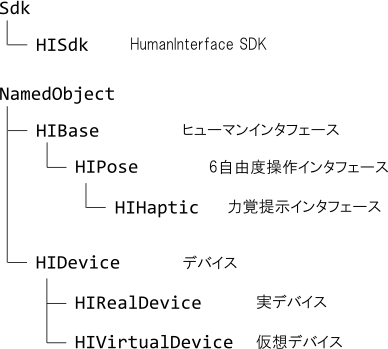
\includegraphics[width=.5\hsize]{fig/hiclass.eps}
\end{center}
\caption{HumanInterface class hierarchy}
\label{fig_hiclass}
\end{figure}

HumanInterface\KLUDGE モジュールのクラス階層をFig.\,\ref{fig_hiclass}\KLUDGE に示します.

\KLUDGE デバイスには実デバイスと仮想デバイスがあります.
\KLUDGE 実デバイスは現実のハードウェアに対応し,例えばWin32\KLUDGE マウスやあるメーカのA/D\KLUDGE 変換ボードを表す実デバイスがあります.
\KLUDGE 一方,仮想デバイスは実デバイスが提供する機能単位を表し,処理系に依存しません.
\KLUDGE 例えば,1\KLUDGE つのA/D\KLUDGE 変換ポートや抽象化されたマウスインタフェースがこれにあたります.
\KLUDGE 基本的に,初期化時を除いてはユーザは実デバイスに触れることはなく,仮想デバイスを通じてそれらの機能を利用することになります.

\KLUDGE ヒューマンインタフェースはデバイスよりも高度で抽象化された操作インタフェースを提供します.


\begin{figure}[t]
\begin{center}
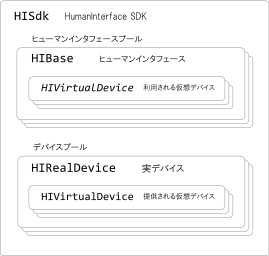
\includegraphics[width=.5\hsize]{fig/humaninterface.eps}
\end{center}
\caption{HumanInterface module data structure}
\label{fig_humaninterface}
\end{figure}

\KLUDGE 次にHumanInterface\KLUDGE モジュールのデータ構造をFig.\,\ref{fig_humaninterface}\KLUDGE に示します.
\texttt{HISdk}\KLUDGE オブジェクトはヒューマンインタフェースプールとデバイスプールを持っています.
\KLUDGE デバイスプールとは実デバイスの集まりで,それぞれの実デバイスはその機能をいくつかの仮想デバイスとして外部に提供します.

\KLUDGE デバイスの機能を使うには,
\begin{enumerate}
\item \KLUDGE 実デバイスを作成する
\item \KLUDGE 実デバイスが提供する仮想デバイスにアクセスする
\end{enumerate}
\KLUDGE という2\KLUDGE 段階の手順を踏みます.
\KLUDGE 以下にそれに関係する\texttt{HISdk}\KLUDGE の関数を紹介します.
\begin{center}
\begin{tabular}{p{.25\hsize}p{.65\hsize}}
\texttt{HISdkIf}																		\\ \midrule
\texttt{HIRealDeviceIf*}	& \texttt{AddRealDevice(const IfInfo* ii, const void* desc = NULL)} \\
\texttt{HIRealDeviceIf*}	& \texttt{FindRealDevice(const char* name)} \\
\texttt{HIRealDeviceIf*}	& \texttt{FindRealDevice(const IfInfo* ii)}
\end{tabular}
\end{center}
\texttt{AddRealDevice}\KLUDGE は型情報\texttt{ii}\KLUDGE とディスクリプタ\texttt{desc}\KLUDGE を指定して実デバイスを作成します.
\texttt{FindRealDevice}\KLUDGE は名前か型情報を指定して,既存の実デバイスを検索します.
\KLUDGE たとえば,内部でGLUT\KLUDGE を用いるキーボード・マウス実デバイスを取得するには
\begin{sourcecode}
hiSdk->FindRealDevice(DRKeyMouseGLUTIf::GetIfInfoStatic());
\end{sourcecode}
\KLUDGE とします.

\KLUDGE 仮想デバイスを取得および返却する方法には\texttt{HISdk}\KLUDGE を介する方法と\texttt{HIRealDevice}\KLUDGE を直接呼び出す方法の2\KLUDGE 通りがあります.
\begin{center}
\begin{tabular}{p{.25\hsize}p{.65\hsize}}
\texttt{HISdkIf}																							\\ \midrule
\texttt{HIVirtualDeviceIf*} & \texttt{RentVirtualDevice(const IfInfo* ii, const char* name, int portNo)}	\\
\texttt{bool}				& \texttt{ReturnVirtualDevice(HIVirtualDeviceIf* dev)}	\\
\end{tabular}
\end{center}
\texttt{RentVirtualDevice}\KLUDGE はデバイスプールをスキャンして型情報に合致した最初の仮想デバイスを返します.
\KLUDGE 実デバイスを限定したい場合は\texttt{name}\KLUDGE で実デバイス名を指定します.
\KLUDGE また,複数の仮想デバイスを提供する実デバイスもあります.
\KLUDGE この場合はポート番号\texttt{portNo}\KLUDGE で取得したい仮想デバイスを指定できます.
%
\KLUDGE デバイスの競合を防ぐために,一度取得された仮想デバイスは利用中状態になります.
\KLUDGE 利用中のデバイスは新たに取得することはできません.
\KLUDGE 使い終わったデバイスは\texttt{ReturnVirtualDevice}\KLUDGE で返却することによって再び取得可能になります.
\begin{center}
\begin{tabular}{p{.25\hsize}p{.65\hsize}}
\texttt{HIRealDeviceIf}																				\\ \midrule
\texttt{HIVirtualDeviceIf*}	& \texttt{Rent(const IfInfo* ii, const char* name, int portNo)}	\\
\texttt{bool}				& \texttt{Return(HIVirtualDeviceIf* dev)}
\end{tabular}
\end{center}
\KLUDGE こちらは実デバイスから直接取得,返却するための関数です.機能は同様です.


\section{\KLUDGE 実デバイス}

Springhead\KLUDGE ではいくつかのメーカ製のハードウェアが実デバイスとしてサポートされていますが,
\KLUDGE 処理系に強く依存する部分であるため本ドキュメントの対象外とします.
\KLUDGE 興味のある方はソースコードを見てください.

\section{\KLUDGE キーボード・マウス}
\label{sec_hi_keymouse}

\KLUDGE キーボードおよびマウスの機能は包括して1\KLUDGE つのクラスとして提供されています.
\KLUDGE キーボード・マウスの仮想デバイスは\texttt{DVKeyMouse}\KLUDGE です.
\KLUDGE 実デバイスとしてはWin32 API\KLUDGE を用いる\texttt{DRKeyMouseWin32}\KLUDGE とGLUT\KLUDGE を用いる\texttt{DRKeyMouseGLUT}\KLUDGE があります.
\KLUDGE 提供される機能に多少の差異があるので注意して下さい.

\subsection*{\KLUDGE 仮想キーコード}

Ascii\KLUDGE 外の特殊キーには処理系依存のキーコードが割り当てられています.
\KLUDGE この差を吸収するために以下のシンボルが\texttt{DVKeyCode}\KLUDGE 列挙型で定義されています.

\begin{center}
\begin{tabular}{p{.3\hsize}p{.6\hsize}}
\texttt{DVKeyCode}									\\ \midrule
\texttt{ESC}				& \KLUDGE エスケープ			\\
\texttt{F1} - \texttt{F12}	& \KLUDGE ファンクションキー	\\
\texttt{LEFT}				& \KLUDGE ←					\\
\texttt{UP}					& \KLUDGE ↑					\\
\texttt{RIGHT}				& \KLUDGE →					\\
\texttt{DOWN}				& \KLUDGE ↓					\\
\texttt{PAGE\_UP}			& Page Up				\\
\texttt{PAGE\_DOWN}			& Page Down				\\
\texttt{HOME}				& Home					\\
\texttt{END}				& End					\\
\texttt{INSERT}				& Insert				\\
\end{tabular}
\end{center}

\KLUDGE 必要に応じてシンボルが追加される可能性がありますので,完全なリストはヘッダファイルで確認してください.

\subsection*{\KLUDGE コールバック}

\texttt{DVKeyMouse}\KLUDGE からのイベントを処理するには\texttt{DVKeyMouseCallback}\KLUDGE クラスを継承し,イベントハンドラをオーバライドします.
\texttt{DVKeyMouseCallback}\KLUDGE はいくつかのヒューマンインタフェースクラスが継承しているほか,
\KLUDGE 後述するアプリケーションクラス\texttt{FWApp}\KLUDGE も継承しています.

\begin{center}
\begin{tabular}{p{.2\hsize}p{.7\hsize}}
\texttt{DVKeyMouseCallback}								\\ \midrule
\texttt{virtual bool} & \texttt{OnMouse(int button, int state, int x, int y)}		\\
\multicolumn{2}{l}{\KLUDGE マウスボタンプッシュ/\KLUDGE リリース}	\\
\\
\texttt{virtual bool} & \texttt{OnDoubleClick(int button, int x, int y)}			\\
\multicolumn{2}{l}{\KLUDGE ダブルクリック}	\\
\\
\texttt{virtual bool} & \texttt{OnMouseMove(int button, int x, int y, int zdelta)}	\\
\multicolumn{2}{l}{\KLUDGE マウスカーソル移動/\KLUDGE マウスホイール回転}	\\
\\
\texttt{virtual bool} & \texttt{OnKey(int state, int key, int x, int y)}			\\
\multicolumn{2}{l}{\KLUDGE キープッシュ/\KLUDGE リリース}	\\
\end{tabular}
\end{center}

\texttt{OnMouse}\KLUDGE はマウスボタンのプッシュあるいはリリースが生じたときに呼び出されます.
\texttt{button}\KLUDGE はイベントに関係するマウスボタンおよびいくつかの特殊キーの識別子を保持し,
\KLUDGE その値は\texttt{DVButtonMask}\KLUDGE 列挙子の値のOR\KLUDGE 結合で表現されます.
\texttt{state}\KLUDGE はマウスボタン状態変化を示し,\texttt{DVButtonSt}\KLUDGE 列挙子のいずれかの値を持ちます.
\texttt{x}\KLUDGE ,\texttt{y}\KLUDGE はイベント生成時のカーソル座標を表します.
\KLUDGE 例として,左ボタンのプッシュイベントを処理するには次のようにします.
\begin{sourcecode}
// inside your class definition ...
virtual bool OnMouse(int button, int state, int x, int y){
    if(button & DVButtonMask::LBUTTON && state == DVButtonSt::DOWN){
        // do something here
    }
}
\end{sourcecode}

\texttt{OnDoubleClick}\KLUDGE はマウスボタンのダブルクリックが生じたときに呼ばれます.
\KLUDGE 引数の定義は\texttt{OnMouse}\KLUDGE と同様です.

\texttt{OnMouseMove}\KLUDGE はマウスカーソルが移動するか,マウスホイールが回転した際に呼ばれます.
\texttt{button}\KLUDGE は直前のマウスプッシュイベントにおいて\texttt{OnMouse}\KLUDGE に渡されたのと同じ値を持ちます.
\texttt{x}, \texttt{y}\KLUDGE は移動後のカーソル座標,\texttt{zdelta}\KLUDGE はマウスカーソルの回転量です.

\texttt{OnKey}\KLUDGE はキーボードのキーがプッシュされるかリリースされた際に呼ばれます.
\texttt{state}\KLUDGE は\texttt{DVKeySt}\KLUDGE 列挙子の値を持ちます.
\texttt{key}\KLUDGE はプッシュあるいはリリースされたキーの仮想キーコードを保持します.

\KLUDGE 以下に関連する列挙子の定義を示します.

\begin{center}
\begin{tabular}{p{.3\hsize}p{.6\hsize}}
\texttt{DVButtonMask}									\\ \midrule
\texttt{LBUTTON}				& \KLUDGE 左ボタン				\\
\texttt{RBUTTON}				& \KLUDGE 右ボタン				\\
\texttt{MBUTTON}				& \KLUDGE 中ボタン				\\
\texttt{SHIFT}					& Shift\KLUDGE キー押し下げ		\\
\texttt{CONTROL}				& Ctrl\KLUDGE キー押し下げ		\\
\texttt{ALT}					& Alt\KLUDGE キー押し下げ		\\
\end{tabular}
\end{center}

\begin{center}
\begin{tabular}{p{.3\hsize}p{.6\hsize}}
\texttt{DVButtonSt}								\\ \midrule
\texttt{DOWN}			& \KLUDGE ボタンプッシュ		\\
\texttt{UP}				& \KLUDGE ボタンリリース		\\
\end{tabular}
\end{center}

\begin{center}
\begin{tabular}{p{.3\hsize}p{.6\hsize}}
\texttt{DVKeySt}								\\ \midrule
\texttt{PRESSED}		& \KLUDGE 押されている			\\
\texttt{TOGGLE\_ON}		& \KLUDGE トグルされている		\\
\end{tabular}
\end{center}

\subsection*{API\KLUDGE として提供される機能}

\KLUDGE 以下に\texttt{DVKeyMouse}\KLUDGE の関数を示します.
\begin{center}
\begin{tabular}{p{.1\hsize}p{.8\hsize}}
\texttt{DVKeyMouseIf}																		\\ \midrule
\texttt{void}	& \texttt{AddCallback(DVKeyMouseCallback*)} 	\\
\texttt{void}	& \texttt{RemoveCallback(DVKeyMouseCallback*)} 	\\
\texttt{int}	& \texttt{GetKeyState(int key)}					\\
\texttt{void}	& \texttt{GetMousePosition(int\& x, int\& y, int\& time, int count=0)}
\end{tabular}
\end{center}
\texttt{AddCallback}\KLUDGE はコールバッククラスを登録します.
\KLUDGE 一つの仮想デバイスに対して複数個のコールバックを登録できます.
\texttt{RemoveCallback}\KLUDGE は登録済のコールバッククラスを解除します.

\texttt{GetKeyState}\KLUDGE は\texttt{DVKeyCode}\KLUDGE で指定したキーの状態を\texttt{DVKeySt}\KLUDGE の値で返します.

\texttt{GetMousePosition}\KLUDGE は\texttt{count}\KLUDGE ステップ前のマウスカーソルの位置を取得するのに用います.
\KLUDGE ただし\texttt{count}\KLUDGE は$0$\KLUDGE 以上$63$\KLUDGE 以下でなければなりません.
\texttt{x}, \texttt{y}\KLUDGE にカーソル座標が,\texttt{time}\KLUDGE にタイムスタンプが格納されます.

\subsection*{\KLUDGE サポート状況に関する注意}

\KLUDGE 使用する実デバイスによっては一部の機能が提供されないので注意して下さい.

\texttt{OnMouseMove}\KLUDGE においてマウスホイールの回転量を取得するには,
\KLUDGE 実デバイスとして\texttt{DRKeyMouseWin32}\KLUDGE を使用するか,
freeglut\KLUDGE とリンクしてビルドしたSpringhead\KLUDGE 上で\texttt{DRKeyMouseGLUT}\KLUDGE を使用する必要があります.

\texttt{OnKey}\KLUDGE においてキーのトグル状態を取得するには
\KLUDGE 実デバイスとして\texttt{DRKeyMouseWin32}\KLUDGE を使用する必要があります.

\texttt{GetKeyState}\KLUDGE は\texttt{DRKeyMouseWin32}\KLUDGE でのみサポートされます.

\texttt{GetMousePosition}\KLUDGE において,タイムスタンプを取得するには\texttt{DRKeyMouseWin32}\KLUDGE を用いる必要があります.

\section{\KLUDGE ジョイスティック}

\KLUDGE ジョイスティックの仮想デバイスは\texttt{DVJoyStick}\KLUDGE です.
\KLUDGE 実デバイスとしてはGLUT\KLUDGE を用いる\texttt{DRJoyStickGLUT}\KLUDGE のみがあります.

T.B.D. 

\section{\KLUDGE トラックボール}

\begin{figure}[t]
\begin{center}
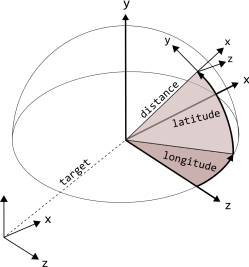
\includegraphics[width=.5\hsize]{fig/hitrackball.eps}
\end{center}
\caption{Trackball}
\label{fig_trackball}
\end{figure}

\KLUDGE トラックボールはキーボード・マウスにより並進・回転の6\KLUDGE 自由度を入力するヒューマンインタフェースです.
\KLUDGE トラックボールを使うことにより,カメラを注視点まわりに視点変更することができるようになります.

\KLUDGE トラックボールを操作する方法には,API\KLUDGE を直接呼び出す方法と,仮想マウスにコールバック登録する方法の二通りがあります.
\KLUDGE 同様に,トラックボールの状態を取得する方法にもAPI\KLUDGE 呼び出しとコールバック登録の二通りがあります.
\KLUDGE 仮想マウスとトラックボールおよびユーザプログラムの関係を\figurename\ref{fig_trackball}\KLUDGE に示します.


\subsection*{\KLUDGE 回転中心と回転角度}

\KLUDGE カメラの位置と向きは,注視点,経度角,緯度角および注視点からの距離によって決まります.

\begin{center}
\begin{tabular}{p{.15\hsize}p{.5\hsize}p{.25\hsize}}
\multicolumn{3}{l}{\texttt{HITrackballDesc}}				\\ \midrule
\texttt{Vec3f}	&	\texttt{target}			& \KLUDGE 回転中心		\\
\texttt{float}	&	\texttt{longitude}		& \KLUDGE 経度[rad]		\\
\texttt{float}	&	\texttt{latitude}		& \KLUDGE 緯度[rad]		\\
\texttt{float}	&	\texttt{distance}		& \KLUDGE 距離			\\
\end{tabular}
\end{center}

\begin{center}
\begin{tabular}{p{.15\hsize}p{.75\hsize}}
\multicolumn{2}{l}{\texttt{HITrackballIf}}									\\ \midrule
\texttt{Vec3f}	& \texttt{GetTarget()}							\\
\texttt{void} 	& \texttt{SetTarget(Vec3f)}						\\
\texttt{void} 	& \texttt{GetAngle(float\& lon, float\& lat)}	\\
\texttt{void} 	& \texttt{SetAngle(float lon, float lat)}		\\
\texttt{float} 	& \texttt{GetDistance()}						\\
\texttt{void} 	& \texttt{SetDistance(float dist)}				\\
\end{tabular}
\end{center}

\subsection*{\KLUDGE 範囲指定}

\KLUDGE 以下の機能で角度および距離に範囲制限を加えられます.

\begin{center}
\begin{tabular}{p{.15\hsize}p{.5\hsize}p{.25\hsize}}
\multicolumn{3}{l}{\texttt{HITrackballDesc}}					\\ \midrule
\texttt{Vec2f}	&	\texttt{lonRange}		& \KLUDGE 経度範囲			\\
\texttt{Vec2f}	&	\texttt{latRange}		& \KLUDGE 緯度範囲			\\
\texttt{Vec2f}	&	\texttt{distRange}		& \KLUDGE 距離範囲			\\
\end{tabular}
\end{center}

\begin{center}
\begin{tabular}{p{.15\hsize}p{.75\hsize}}
\multicolumn{2}{l}{\texttt{HITrackballIf}}									\\ \midrule
\texttt{void} 	& \texttt{GetLongitudeRange(float\& rmin, float\& rmax)}	\\
\texttt{void} 	& \texttt{SetLongitudeRange(float rmin, float rmax)}		\\
\texttt{void} 	& \texttt{GetLatitudeRange(float\& rmin, float\& rmax)}		\\
\texttt{void} 	& \texttt{SetLatitudeRange(float rmin, float rmax)}			\\
\texttt{void} 	& \texttt{GetDistanceRange(float\& rmin, float\& rmax)}		\\
\texttt{void} 	& \texttt{SetDistanceRange(float rmin, float rmax)}			\\
\end{tabular}
\end{center}

\subsection*{\KLUDGE コールバック登録}

\begin{center}
\begin{tabular}{p{.2\hsize}p{.7\hsize}}
\multicolumn{2}{l}{\texttt{HITrackballIf}}								\\ \midrule
\texttt{DVKeyMouseIf*} 	& \texttt{GetKeyMouse()}						\\
\texttt{void} 			& \texttt{SetKeyMouse(DVKeyMouseIf*)}			\\
\texttt{void} 			& \texttt{SetCallback(HITrackballCallback*)}	\\
\end{tabular}
\end{center}

\KLUDGE トラックボールをマウス操作するには\texttt{DVKeyMouse}\KLUDGE クラスにコールバック登録する必要があります.
\KLUDGE コールバック登録するには\texttt{SetKeyMouse}\KLUDGE ,登録先の仮想マウスを取得するには\texttt{GetKeyMouse}\KLUDGE を呼びます.

\KLUDGE また,ユーザプログラムがトラックボールにコールバック登録して状態変化に反応できるようにするには,
\texttt{HITrackballCallback}\KLUDGE クラスを継承し,\texttt{SetCallback}\KLUDGE 関数に渡します.
\texttt{HITrackballCallback}\KLUDGE は以下の単一の仮想関数を持ちます.
\begin{center}
\begin{tabular}{p{.2\hsize}p{.7\hsize}}
\multicolumn{2}{l}{\texttt{HITrackballCallback}}					\\ \midrule
\texttt{virtual void} 	& \texttt{OnUpdatePose(HITrackballIf* tb)}	\\
\end{tabular}
\end{center}
\texttt{OnUpdatePose}\KLUDGE はトラックボールの位置・向きに変化が生じる度に呼ばれます.
\KLUDGE 引数の\texttt{tb}\KLUDGE は呼び出し元のトラックボールを示します.

\subsection*{\KLUDGE マウスボタン割当て}

\texttt{HITrackball}\KLUDGE は内部で\texttt{DVKeyMouseCallback}\KLUDGE を継承します.
\texttt{SetKeyMouse}\KLUDGE により\texttt{DVKeyMouse}\KLUDGE にコールバック登録すると,
\KLUDGE マウスカーソルが移動するたびに\texttt{OnMouseMove}\KLUDGE イベントハンドラが呼び出され,トラックボールの内部状態が更新されます.
\KLUDGE マウス移動時のボタン状態に応じてトラックボールのどの状態が変化するかはある程度カスタマイズが可能です.
\KLUDGE 以下に関連する機能を示します.

\begin{center}
\begin{tabular}{p{.15\hsize}p{.35\hsize}p{.4\hsize}}
\multicolumn{3}{l}{\texttt{HITrackballDesc}}		\\ \midrule
\texttt{int}	& \texttt{rotMask}		& \KLUDGE 回転操作のボタン割当て		\\
\texttt{int}	& \texttt{zoomMask}		& \KLUDGE ズーム操作のボタン割当て		\\
\texttt{int}	& \texttt{trnMask}		& \KLUDGE 平行移動操作のボタン割当て	\\
\end{tabular}
\end{center}

\begin{center}
\begin{tabular}{p{.15\hsize}p{.75\hsize}}
\multicolumn{2}{l}{\texttt{HITrackballIf}}			\\ \midrule
\texttt{void} 	& \texttt{SetRotMask(int mask)}		\\
\texttt{void} 	& \texttt{SetZoomMask(int mask)}	\\
\texttt{void} 	& \texttt{SetTrnMask(int mask)}		\\
\end{tabular}
\end{center}

\texttt{rotMask}, \texttt{zoomMask}, \texttt{trnMask}\KLUDGE はそれぞれ
\KLUDGE 回転操作,ズーム操作,平行移動操作に割り当てたいマウスボタンに対応する
\texttt{OnMouseMove}\KLUDGE の\texttt{button}\KLUDGE 引数の値を表します.
\KLUDGE 以下に対応関係をまとめます.
\begin{center}
\begin{tabular}{p{.3\hsize}p{.3\hsize}p{.3\hsize}}
\toprule
\KLUDGE マウス移動方向		& \texttt{button}\KLUDGE 値		& \KLUDGE 変化量		\\ \midrule
\KLUDGE 左右				& \texttt{rotMask}		& \KLUDGE 経度			\\
\KLUDGE 上下				& \texttt{rotMask}		& \KLUDGE 緯度			\\
\KLUDGE 上下				& \texttt{zoomMask}		& \KLUDGE 距離			\\
\KLUDGE 左右				& \texttt{trnMask}		& \KLUDGE 注視点x\KLUDGE 座標	\\
\KLUDGE 上下				& \texttt{trnMask}		& \KLUDGE 注視点y\KLUDGE 座標	\\
\bottomrule
\end{tabular}
\end{center}
\KLUDGE デフォルトのボタン割当ては以下の通りです.
\begin{center}
\begin{tabular}{p{.3\hsize}p{.6\hsize}}
\texttt{rotMask}	& \texttt{LBUTTON}					\\
\texttt{zoomMask}	& \texttt{RBUTTON}					\\
\texttt{trnMask}	& \texttt{LBUTTON} + \texttt{ALT}	\\
\end{tabular}
\end{center}
\KLUDGE したがって,左ボタンドラッグで回転操作,右ボタンドラッグでズーム操作,[ALT]\KLUDGE キー+\KLUDGE 左ドラッグで平行移動となります.

\KLUDGE なお,現状ではマウスの移動方向との対応をカスタマイズすることはできません.
\KLUDGE また,マウスホイールの回転とトラックボールを連動させる機能も未実装です.

\subsection*{\KLUDGE マウス操作に対する極性と感度}

\KLUDGE マウス移動量と角度変化量,距離変化量との比例係数を下記の機能で設定できます.

\begin{center}
\begin{tabular}{p{.15\hsize}p{.35\hsize}p{.4\hsize}}
\multicolumn{3}{l}{\texttt{HITrackballDesc}}							\\ \midrule
\texttt{float}	&	\texttt{rotGain}		& \KLUDGE 回転ゲイン[rad/pixel]		\\
\texttt{float}	&	\texttt{zoomGain}		& \KLUDGE ズームゲイン[rad/pixel]	\\
\texttt{float}	&	\texttt{trnGain}		& \KLUDGE 平行移動ゲイン			\\
\end{tabular}
\end{center}

\begin{center}
\begin{tabular}{p{.15\hsize}p{.75\hsize}}
\multicolumn{2}{l}{\texttt{HITrackballIf}}									\\ \midrule
\texttt{float} 	& \texttt{GetRotGain()}			\\
\texttt{void} 	& \texttt{SetRotGain(float g)}	\\
\texttt{float} 	& \texttt{GetZoomGain()}		\\
\texttt{void} 	& \texttt{SetZoomGain(float g)}	\\
\texttt{float} 	& \texttt{GetTrnGain()}			\\
\texttt{void} 	& \texttt{SetTrnGain(float g)}	\\
\end{tabular}
\end{center}

\subsection*{\KLUDGE トラックボールで視点を動かす}

\KLUDGE トラックボールの位置と向きをカメラに反映するには,
\KLUDGE 描画処理の冒頭で以下のようにします.

\begin{sourcecode}
// given GRRenderIf* render
render->SetViewMatrix(trackball->GetAffine().inv());
\end{sourcecode}

\section{Spidar}

Spidar\KLUDGE はワイヤ駆動型の3\KLUDGE 軸・6\KLUDGE 軸力覚提示ヒューマンインタフェースです.

T.B.D. 




\chapter{Creature}
\label{chap_creature}
\begin{chapterabstract}
Creature\KLUDGE モジュールは,物理シミュレータを用いてバーチャルクリーチャ(自律動作するキャラクタ)を作成する機能を提供します.

Springhead\KLUDGE の物理シミュレーション機能は,人間・動物・キャラクタ・ロボット等の身体動作をシミュレーションすることにおいても利用価値があります.
\KLUDGE 剛体・関節系で身体モデルを作成し,関節に組み込まれた制御機能や関節系のIK\KLUDGE 機能を用いて身体動作を生成することができます.
\KLUDGE 物理シミュレータ内の情報(物体の運動・形状・接触力等)を利用してバーチャルな感覚(センサ)情報の生成もできます.感覚・制御のループを回すことで自律動作するキャラクタやロボットが実現できます.

\KLUDGE こうしたバーチャルなキャラクタ・ロボット等を総称して,バーチャルクリーチャ(Creature : \KLUDGE 生き物)と呼びます.
\end{chapterabstract}

% ----- ----- ----- ----- ----- ----- ----- ----- ----- ----- ----- ----- ----- ----- ----- ----- ----- ----- ----- -----
%
% \KLUDGE <ドキュメントの書き方>

% \KLUDGE 機能 ::= "\KLUDGE 概説" \KLUDGE 例 \KLUDGE 詳細 \KLUDGE リファレンス*
% \KLUDGE 例   ::= ["\KLUDGE コード例" "\KLUDGE コード例の説明"]*
% \KLUDGE 詳細 ::= [\KLUDGE 機能]*

% \KLUDGE リファレンス ::= [\KLUDGE ディスクリプタ | \KLUDGE インタフェース]

% - \KLUDGE 原則としてリファレンスは機能のまとめと補遺にとどめる.
% - Getter/Setter\KLUDGE は対応するディスクリプタのリファレンスに書き,インタフェースのリファレンスには載せない.
% - \KLUDGE 図は "\KLUDGE 概説" "\KLUDGE コード例" "\KLUDGE コード例の説明" \KLUDGE で適宜用いる.ただし "\KLUDGE コード例" \KLUDGE の図は原則としてそのコードの実行結果とする.

%
% ----- ----- ----- ----- ----- ----- ----- ----- ----- ----- ----- ----- ----- ----- ----- ----- ----- ----- ----- -----


% ----- ----- ----- ----- ----- ----- ----- ----- ----- ----- ----- ----- ----- ----- ----- ----- ----- -----
%
% \KLUDGE 概説
% 

\section{Creature\KLUDGE モジュールの構成}

\KLUDGE 下図にCreature\KLUDGE モジュールのシーンツリー構造を示します。

\begin{sourcecode}
CRSdk
+-- CRCreature
|   +-- CRBody
|   |   +-- CRBone
|   +-- CREngine (CRSensor, CRController)
\end{sourcecode}

\texttt{CRSdk}\KLUDGE はCreature\KLUDGE の機能を使用する根本となるオブジェクトです。
\begin{sourcecode}
CRSdkIf* crSdk = CRSdkIf::CreateSdk();
\end{sourcecode}

\texttt{CRCreature}\KLUDGE は,バーチャルクリーチャ$1$\KLUDGE 体分の機能を統括するオブジェクトです.身体、感覚器、制御器を有しています.CRCreatureDesc\KLUDGE には特に設定すべき項目はありません。
\begin{sourcecode}
CRCreatureIf* crCreature = crSdk->CreateCreature(
  CDCreatureIf::GetIfInfoStatic(), CRCreatureDesc());
\end{sourcecode}
CRCreature\KLUDGE を作成したら、物理シミュレーションのシーンと関連づけるために、PHScene\KLUDGE を子オブジェクトとしてセットしてください。
\begin{sourcecode}
// PHSceneIf* phScene;   // should be taken from somewhere
crCreature->AddChildObject(phScene);
\end{sourcecode}

\KLUDGE シミュレーション実行時は、1\KLUDGE ステップに1\KLUDGE 回、CRCreature\KLUDGE のStep\KLUDGE を呼んでください。これを呼ぶとCreature\KLUDGE が持つ各Engine\KLUDGE のStep\KLUDGE が実行されます。
\begin{sourcecode}
// Every time after simulation step
crCreature.Step();
\end{sourcecode}



\subsection{\KLUDGE 身体}

\texttt{CRBody}\KLUDGE は,バーチャルクリーチャの身体モデルを統括します.身体モデルは身体構成部品の集合体です.
\begin{sourcecode}
CDBodyIf* crBody = crCreature->CreateBody(
  CRBodyIf::GetIfInfoStatic(), CRBodyDesc());
\end{sourcecode}

\texttt{CRBone}\KLUDGE は,身体構成部品ひとつひとつに対応するオブジェクトです.剛体と関節、IK\KLUDGE のためのアクチュエータ(場合によってはエンドエフェクタ)をセットにしたものです。
\begin{sourcecode}
CRBoneIf* crBone = crBody->CreateObject(
  CDBoneIf::GetIfInfoStatic(), CRBoneDesc());
\end{sourcecode}
CRBone\KLUDGE に関連づけるべきオブジェクトはすべて子オブジェクトとしてください。
\begin{sourcecode}
// このBoneに対応する剛体
// PHSolidIf* phSolid; 
crBone->AddChildObject(phSolid);

// このBoneを親Boneに接続する関節。Root Boneの場合は存在しないので追加不要。
// PHJointIf* phJoint;
crBone->AddChildObject(phJoint);

// IKのエンドエフェクタ(手先など)である場合は対応するPHIKEndEffector
// PHIKEndEffectorIf* phIKEEff;
crBone->AddChildObject(phIKEEff);

// phJointに対応するIKアクチュエータ
// PHIKActuatorIf* phIKAct;
crBone->AddChildObject(phIKAct);
\end{sourcecode}


\subsection{\KLUDGE 感覚器}

\KLUDGE 感覚器(CRSensor)\KLUDGE はCREngine\KLUDGE の一種です。\texttt{CREngine}\KLUDGE は,バーチャルクリーチャのステップ処理の実行主体です.\texttt{CRCreature}\KLUDGE の\texttt{Step}\KLUDGE 関数が1\KLUDGE 回呼ばれるたびに,\texttt{CRCreature}\KLUDGE が保持する全ての\texttt{CREngine}\KLUDGE の\texttt{Step}\KLUDGE 関数が順に実行されます.

CRSensor\KLUDGE には視覚(CRVisualSensor\KLUDGE )、触覚(CRTouchSensor\KLUDGE )があります。

\paragraph{\KLUDGE 視覚}

\KLUDGE 視野内にある剛体を1Step\KLUDGE ごとにリストアップする機能です。
\begin{sourcecode}
// 設定
CRVisualSensorDesc descVisualSensor;
/// 視野の大きさ: 水平角度,垂直角度
descVisualSensor.range = Vec2d(Rad(90), Rad(60));
// 中心視野の大きさ: 水平角度,垂直角度
descVisualSensor.centerRange = Vec2d(Rad(10), Rad(10));
// 視覚センサを対象剛体に貼り付ける位置・姿勢
descVisualSensor.pose = Posed();
// この距離を越えたものは視野外        
descVisualSensor.limitDistance = 60;	

// 作成
CRVisualSensorIf* crVisualSensor = crCreature->CreateEngine(
  CRVisualSensorIf::GetIfInfoStatic(), descVisualSensor);
\end{sourcecode}

\KLUDGE 視覚情報を読み出すには NVisibles() \KLUDGE と GetVisible(int n) \KLUDGE を用います。視覚情報を利用する前には必ずUpdate\KLUDGE を実行してください。Update\KLUDGE を実行すると視覚情報が最新のStep\KLUDGE に基づく情報に更新されます。
\begin{sourcecode}
crVisualSensor->Update();
for (int i=0; i<crVisualSensor->NVisibles(); ++i) {
	CRVisualInfo info = crVisualSensor->GetVisible(i);
	// 可視剛体一個分の視覚情報
	info.posWorld;    // 可視剛体のワールド座標
	info.posLocal;    // 頭を基準とした可視剛体のローカル座標
	info.velWorld;    // 速度
	info.velLocal;    // ローカル座標での速度
	info.angle;       // 視野中心から剛体までの視角(たぶん)
	info.solid;       // 可視剛体
	info.solidSensor; // 視覚センサ剛体(頭とか目とか)
	info.sensorPose;  // 視覚センサ剛体の位置・姿勢(たぶん)
	info.bMyBody;     // 自分の身体を構成する剛体であればtrue
	info.bCenter;     // 中心視野に入っていればtrue
}
\end{sourcecode}


\subsection{\KLUDGE 制御器}

\texttt{CRController}\KLUDGE は\texttt{CREngine}\KLUDGE の一種で,バーチャルクリーチャの身体制御を担当します.実際の制御機能は\texttt{CRController}\KLUDGE を継承した各クラスが担当します.到達運動制御、眼球運動制御などがあります。



\chapter{Framework}
\label{chap_framework}
\section{\KLUDGE 概要}

\index{Framework}

\begin{figure}[t]
\begin{center}
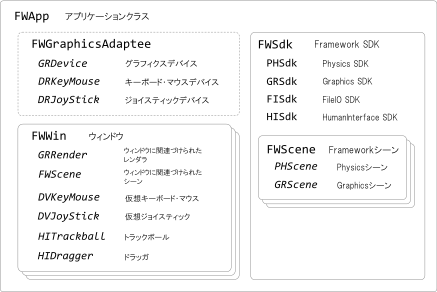
\includegraphics[width=.7\hsize]{fig/framework.eps}
\end{center}
\caption{Framework data structure}
\label{fig_framework}
\end{figure}


Framework\KLUDGE はモジュール間の連携を促進してアプリケーションの作成を支援するためのモジュールです.

Framework\KLUDGE モジュールのデータ構造をFig.\,\ref{fig_framework}\KLUDGE に示します.
\KLUDGE 最上位にはアプリケーションクラス\texttt{FWApp}\KLUDGE があります.
\KLUDGE ユーザは\texttt{FWApp}\KLUDGE を継承することで独自のアプリケーションを作成します.
\texttt{FWApp}\KLUDGE その中にトップレベルウィンドウ(\texttt{FWWin})\KLUDGE の配列,Framework SDK (\texttt{FWSdk})\KLUDGE ,
\KLUDGE およびウィンドウマネジャ(\texttt{FWGraphicsAdaptee})\KLUDGE を持ちます.

\texttt{FWWin}\KLUDGE はトップレベルウィンドウで,そのウィンドウに対応する入力デバイスやビューポート情報を保持するレンダラ,
\KLUDGE そのウィンドウと関連付けられたシーンへの参照などを持ちます.
\KLUDGE また,図中では省略されていますがサブウィンドウやGUI\KLUDGE コントロールを持つこともできます.

\texttt{FWSdk}\KLUDGE の役割は周辺モジュールの機能統合です.
\KLUDGE その中に周辺モジュールのSDK\KLUDGE クラスやFramework\KLUDGE シーン(\texttt{FWScene})\KLUDGE の配列を持ちます.

\KLUDGE ウィンドウマネジャは処理系に依存するデバイスの初期化やイベントハンドリングを行います.
\KLUDGE ウィンドウマネジャはインタフェースを公開していませんのでユーザはその存在を陽に意識する必要はありません.
\KLUDGE 図ではデータ構造の説明のためにあえて記載しています.

\KLUDGE 以下では個々の構成要素について説明していきます.


\section{Framework SDK}

\index{FWSdk}
Framework\KLUDGE モジュールのすべてのオブジェクトはSDK\KLUDGE クラス\texttt{FWSdk}\KLUDGE によって管理されます.
\texttt{FWSdk}\KLUDGE クラスは,プログラムの実行を通してただ1つのオブジェクトが存在するシングルトンクラスです.
\texttt{FWSdk}\KLUDGE オブジェクトを作成するには以下のようにします.
\begin{sourcecode}
FWSdkIf* fwSdk = FWSdkIf::CreateSdk();
\end{sourcecode}
\KLUDGE 通常この操作はプログラムの初期化時に一度だけ実行します.
\texttt{FWSdk}\KLUDGE を作成すると,同時に\texttt{PHSdk}\KLUDGE ,\texttt{GRSdk}\KLUDGE ,\texttt{FISdk}\KLUDGE ,\texttt{HISdk}\KLUDGE も作成されます.
\KLUDGE したがってこれらをユーザが手動で作成する必要はありません.
\KLUDGE 各モジュールの機能にアクセスするには以下の関数によりSDK\KLUDGE を取得します.

\noindent
\begin{tabular}{p{1.0\hsize}}
\\
\texttt{FWSdkIf}				\\ \midrule
\texttt{PHSdkIf* GetPHSdk()}	\\
Physics SDK\KLUDGE を取得する.			\\
\\
\texttt{GRSdkIf* GetGRSdk()}	\\
Graphics SDK\KLUDGE を取得する.		\\
\\
\texttt{FISdkIf* GetFISdk()}	\\
FileIO SDK\KLUDGE を取得する.			\\
\\
\texttt{HISdkIf* GetHISdk()}	\\
HumanInterface SDK\KLUDGE を取得する.	\\
\\
\end{tabular}

\section{Framework \KLUDGE シーン}

\begin{figure}[t]
\begin{center}
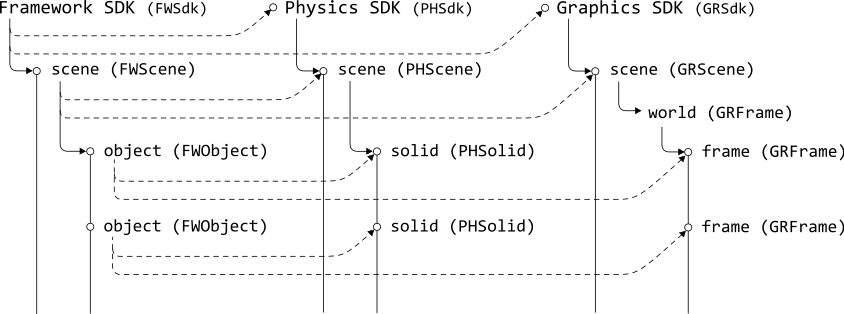
\includegraphics[width=.9\hsize]{fig/fwscene.eps}
\end{center}
\caption{Data structure of Framework, Physics and Graphics modules}
\label{fig_fwscene}
\end{figure}

\index{FWScene}
\index{FWObject}
Framework\KLUDGE モジュールの主な機能の1\KLUDGE つにPhysics\KLUDGE シーンとGraphics\KLUDGE シーンの同期があります.
Fig.\,\ref{fig_fwscene}\KLUDGE に3\KLUDGE つのモジュールのSDK\KLUDGE とシーンの関係を示します.
\texttt{FWSdk}\KLUDGE は任意の数のシーン(\texttt{FWScene}\KLUDGE クラス)を保持します.
\KLUDGE また,シーンは任意の数のオブジェクト(\texttt{FWObject}\KLUDGE クラス)を保持します.
Fig.\,\ref{fig_fwscene}\KLUDGE に示すように,
\KLUDGE オブジェクトはPhysics\KLUDGE モジュールの剛体とGraphics\KLUDGE モジュールのトップフレームを一対一に対応づけます.
\KLUDGE ここでトップフレームとはワールドフレームの直下にあるフレームのことです.
\KLUDGE 物理シミュレーションにより計算される剛体の運動をフレームの座標変換に反映させることで,
\KLUDGE シミュレーションの様子をGraphics\KLUDGE モジュールの機能を利用して可視化することができるようになります.

\KLUDGE シーン作成に関する\texttt{FWSdk}\KLUDGE の関数を以下に示します.

\noindent
\begin{tabular}{p{1.0\hsize}}
\\
\texttt{HITrackballIf}														\\ \midrule
\texttt{FWSceneIf* CreateScene(const PHSceneDesc\&, const GRSceneDesc\&)}	\\
\KLUDGE シーンを作成する.															\\
\\
\texttt{int NScene()}	\\
\KLUDGE シーンの数を取得する	\\
\\
\texttt{FWSceneIf* GetScene(int i)}	\\
\texttt{i}\KLUDGE 番目のシーンを取得する.	\\
\\
\texttt{void MergeScene(FWSceneIf* scene0, FWSceneIf* scene1)}	\\
\texttt{scene1}\KLUDGE の子オブジェクトを\texttt{scene0}\KLUDGE に移す.		\\
\\
\end{tabular}

\KLUDGE シーンを作成するには以下のようにします.
\begin{sourcecode}
FWSceneIf* fwScene = fwSdk->CreateScene();
\end{sourcecode}
\texttt{FWScene}\KLUDGE を作成すると,同時に\texttt{PHScene}\KLUDGE と\texttt{GRScene}\KLUDGE も作成され,\texttt{FWScene}\KLUDGE とリンクされます.
\texttt{CreateScene}\KLUDGE にディスクリプタを指定することもできます.
\texttt{NScene}\KLUDGE は作成したシーンの数を返します.

%\KLUDGE シーンはいくつでも作成できますが,その中の1\KLUDGE つのシーンが選択された状態にあります.
%\KLUDGE 選択されたシーンをカレントシーンと呼びます.
%\KLUDGE 新しく作成されたシーンはカレントシーンとなります.
%\KLUDGE 選択を切り替えるには\texttt{SwitchScene}\KLUDGE を使います.

\KLUDGE シーンを取得するには\texttt{GetScene}\KLUDGE を使います.
\texttt{GetScene}\KLUDGE に指定する整数は作成された順番にシーンに与えられる通し番号です.
%\KLUDGE 引数を省略するとカレントシーンが返されます.
\begin{sourcecode}
fwSdk->CreateScene();               // create two scenes
fwSdk->CreateScene();
FWSceneIf *fwScene0, *fwScene1;
fwScene0 = fwSdk->GetScene(0);      // get 1st scene
fwScene1 = fwSdk->GetScene(1);      // get 2nd scene
\end{sourcecode}

\texttt{MergeScene}\KLUDGE を使うと2\KLUDGE つのシーンを統合して1\KLUDGE つのシーンにできます.
\begin{sourcecode}
fwSdk->MergeScene(fwScene0, fwScene1);
\end{sourcecode}
\KLUDGE 上のコードでは\texttt{scene1}\KLUDGE が持つ\texttt{FWObject}\KLUDGE が\texttt{scene0}\KLUDGE に移され,同時にシーンが参照する
\texttt{PHScene}\KLUDGE と\texttt{GRScene}\KLUDGE に関してもそれぞれの\texttt{MergeScene}\KLUDGE 関数により統合が行われます.

\KLUDGE 次に,\texttt{FWScene}\KLUDGE の基本機能を以下に示します.

\noindent
\begin{tabular}{p{.6\hsize}p{.3\hsize}}
\\
\texttt{FWSceneIf}													\\ \midrule
\texttt{void SetPHScene(PHSceneIf*)}	& Physics\KLUDGE シーンの設定		\\
\texttt{PHSceneIf* GetPHScene()}		& Physics\KLUDGE シーンの取得		\\
\texttt{void SetGRScene(GRSceneIf*)}	& Graphics\KLUDGE シーンの設定		\\
\texttt{GRSceneIf* GetGRScene()}		& Graphics\KLUDGE シーンの取得		\\
\texttt{FWObjectIf* CreateFWObject()}	& \KLUDGE オブジェクトの作成		\\
\texttt{int NObject()const}				& \KLUDGE オブジェクトの数			\\
\texttt{FWObjectIf** GetObjects()}		& \KLUDGE オブジェクト配列の取得	\\
\texttt{void Sync(bool)}				& \KLUDGE 同期						\\
\\
\end{tabular}

\texttt{[Set|Get][PH|GR]Scene}\KLUDGE 関数はシーンに割り当てられた\texttt{PHScene}\KLUDGE や\texttt{GRScene}\KLUDGE を取得したり,別のシーンを割り当てたりするのに使用します.

\texttt{CreateFWObject}\KLUDGE 関数は\texttt{FWObject}\KLUDGE オブジェクトを作成します.
\KLUDGE このとき,新たに作成された\texttt{FWObject}\KLUDGE には\texttt{PHSolid}\KLUDGE および\texttt{GRFrame}\KLUDGE は割り当てられていない状態になっているので注意してください.
\KLUDGE これらも同時に作成するには,以下のコードを1\KLUDGE セットで実行します.

\begin{sourcecode}
FWObjectIf* fwObj = fwScene->CreateFWObject();
fwObj->SetPHSolid(fwScene->GetPHScene()->CreateSolid());
fwObj->SetGRFrame(
    fwScene->GetGRScene()->CreateVisual(GRFrameDesc())->Cast);
\end{sourcecode}

\texttt{Sync}\KLUDGE 関数は\texttt{PHScene}\KLUDGE と\texttt{GRScene}\KLUDGE の同期に用います.
\begin{sourcecode}
fwScene->Sync(true);
\end{sourcecode}
\KLUDGE とすると,このシーンが参照する\texttt{PHScene}\KLUDGE 中の剛体の位置と向きが,
\KLUDGE 同じくこのシーンが参照する\texttt{GRScene}\KLUDGE 中のトップフレームの位置と向きに反映されます.
\KLUDGE このときの剛体とトップフレームとの対応関係は\texttt{FWObject}\KLUDGE により定義されます.

\KLUDGE 逆に
\begin{sourcecode}
fwScene->Sync(false);
\end{sourcecode}
\KLUDGE とすると,同様のメカニズムで各トップフレームの位置と向きが対応する剛体に反映されます.

\section{\KLUDGE シーンのロードとセーブ}

FileIO\KLUDGE モジュールを利用してシーンをロード,セーブするための関数が用意されています.
\KLUDGE まずロードには以下の関数を用います.

\noindent
\begin{tabular}{p{1.0\hsize}}
\\
\texttt{FWSdkIf}														\\ \midrule
\texttt{bool LoadScene(UTString path, ImportIf* imp, const IfInfo* ii, ObjectIfs* objs)}	\\
\KLUDGE シーンをロードする.		\\
\\
\end{tabular}

\texttt{path}\KLUDGE はロードするファイルへのパスを格納した文字列です.
\texttt{imp}\KLUDGE にはインポート情報を格納するための\texttt{Import}\KLUDGE オブジェクトを与えます.
\KLUDGE インポート情報を記憶する必要のない場合は\texttt{NULL}\KLUDGE で構いません.
\texttt{ii}\KLUDGE はロードするファイルの種類を明示するための型情報です.
\texttt{NULL}\KLUDGE を指定するとパスの拡張子から自動判別されます.
\texttt{objs}\KLUDGE はロードによって作成されるオブジェクトツリーの親オブジェクトを格納した配列です.

\KLUDGE ロードに成功すると\texttt{true}\KLUDGE ,失敗すると\texttt{false}\KLUDGE が返されます.
\KLUDGE ロードされたシーンは\texttt{FWSdk}\KLUDGE のシーン配列の末尾に加えられます.

\KLUDGE 次に,シーンをセーブするには以下の関数を使います.

\noindent
\begin{tabular}{p{1.0\hsize}}
\\
\texttt{FWSdkIf}														\\ \midrule
\texttt{bool SaveScene(UTString path, ImportIf* imp, const IfInfo* ii, ObjectIfs* objs)}	\\
\KLUDGE シーンをセーブする.		\\
\\
\end{tabular}

\KLUDGE 引数の意味は\texttt{LoadScene}\KLUDGE と同様です.
\texttt{imp}\KLUDGE にはロード時に記憶したインポート情報を与えます.
\KLUDGE 省略するとシーン全体が単一のファイルにセーブされます.

\KLUDGE セーブに成功すると\texttt{true}\KLUDGE ,失敗すると\texttt{false}\KLUDGE が返されます.


\section{Framework \KLUDGE オブジェクト}

\texttt{FWObject}\KLUDGE は\texttt{PHSolid}\KLUDGE と\texttt{GRFrame}\KLUDGE の橋渡しが主な役割ですので,それ自体はそれほど多くの機能を持っていません.


\section{\KLUDGE アプリケーションクラス}

\index{FWApp}
Springhead\KLUDGE を利用するアプリケーションの作成を容易にするために,アプリケーションクラス\texttt{FWApp}\KLUDGE が用意されています.
\ref{sec_create_application}\KLUDGE に\texttt{FWApp}\KLUDGE を使って簡単なアプリケーションを作成する方法について説明しましたのでそちらも合わせて参考にしてください.

\KLUDGE 冒頭で説明した通り,Springhead\KLUDGE のほとんどのオブジェクトは,親オブジェクトの\texttt{Create}\KLUDGE 系関数を使って作成しますが,
\texttt{FWApp}\KLUDGE は例外的に,C++\KLUDGE のクラス継承を用いてユーザのアプリケーションクラスを定義する方法をとります.
\KLUDGE この方が仮想関数によって動作のカスタマイズがフレキシブルに行えるからです.

\KLUDGE 以下では\texttt{FWApp}\KLUDGE の機能やユーザが実装すべき仮想関数について順に見ていきます.

\subsection*{\KLUDGE 初期化}

\texttt{FWApp}\KLUDGE の初期化処理は仮想関数\texttt{Init}\KLUDGE で行います.

\noindent
\begin{tabular}{p{.7\hsize}p{.2\hsize}}
\\
\texttt{FWApp}											\\ \midrule
\texttt{virtual void Init(int argc, char* argv[])}	&	\\
\\
\end{tabular}

\KLUDGE 以下に\texttt{Init}\KLUDGE 関数のデフォルトの実装を示します.

\begin{sourcecode}
void FWApp::Init(int argc, char* argv[]){
    // create SDK
    CreateSdk();
    // create a single scene
    GetSdk()->CreateScene();
    // initialize window manager
    GRInit(argc, argv);
    // create main window
    CreateWin();
    // create timer
    CreateTimer();
}
\end{sourcecode}
\KLUDGE はじめに
\begin{sourcecode}
    CreateSdk();
\end{sourcecode}
\KLUDGE でSDK\KLUDGE を作成します.
\KLUDGE つぎに
\begin{sourcecode}
    GRInit(argc, argv);
\end{sourcecode}
\KLUDGE でウィンドウマネジャが作成されます.
\KLUDGE デフォルトではGLUT\KLUDGE を用いるウィンドウマネジャが作成されます.
\KLUDGE さらに
\begin{sourcecode}
    GetSdk()->CreateScene();
\end{sourcecode}
\KLUDGE で\texttt{FWScene}\KLUDGE を1\KLUDGE つ作成します.
\KLUDGE つづいて
\begin{sourcecode}
    CreateWin();
\end{sourcecode}
\KLUDGE でメインウィンドウを作成します.
\KLUDGE 最後に
\begin{sourcecode}
    CreateTimer();
\end{sourcecode}
\KLUDGE でタイマを作成します.

\KLUDGE この基本処理に追加してなんらかの処理を行う場合は
\begin{sourcecode}
virtual void Init(int argc = 0, char* argv[] = 0){
    // select GLUI window manager
    SetGRAdaptee(TypeGLUI);

    // call base Init
    FWApp::Init(argc, argv);

    // do extra initialization here


}
\end{sourcecode}
\KLUDGE のように,\texttt{FWApp:Init}\KLUDGE を実行してから追加の処理を行うのが良いでしょう.
\KLUDGE 一方,以下に挙げるようなカスタマイズが必要な場合は\texttt{Init}\KLUDGE 関数の処理全体を派生クラスに記述する必要があります.
\begin{itemize}
\item \KLUDGE シーン生成をカスタマイズしたい
\item \KLUDGE ウィンドウの初期サイズやタイトルを変更したい
\item \KLUDGE 異なる種類のタイマが使いたい
\end{itemize}
\KLUDGE この場合は,上に載せた\texttt{Init}\KLUDGE のデフォルト処理をもとに必要な部分に修正を加えるのが良いでしょう.

\KLUDGE プログラムの全体の構造は通常以下のようになります.

\begin{sourcecode}
MyApp app;

int main(int argc, char* argv[]){
    app.Init(argc, argv);
    app.StartMainLoop();
    return 0;
}
\end{sourcecode}

\KLUDGE ここで\texttt{MyApp}\KLUDGE はユーザが定義した\texttt{FWApp}\KLUDGE の派生クラスです(もちろん他の名前でも構いません).
\texttt{MyApp}\KLUDGE のインスタンスをグローバル変数として定義し,
\texttt{main}\KLUDGE 関数で\texttt{Init}\KLUDGE ,\texttt{StartMainLoop}\KLUDGE を順次実行します.
\texttt{StartMainLoop}\KLUDGE 関数はアプリケーションのメインループを開始します.


\subsection*{\KLUDGE タイマ}

\KLUDGE タイマの作成には\texttt{CreateTimer}\KLUDGE 関数を使います.
\KLUDGE 通常,\texttt{CreateTimer}\KLUDGE は\texttt{Init}\KLUDGE の中で呼びます.

\noindent
\begin{tabular}{p{.7\hsize}p{.2\hsize}}
\\
\texttt{FWApp}												\\ \midrule
\texttt{UTTimerIf* CreateTimer(UTTimerIf::Mode mode)}	&	\\
\\
\end{tabular}

\KLUDGE 引数\texttt{mode}\KLUDGE に指定できる値は\texttt{UTTimer}\KLUDGE の\texttt{SetMode}\KLUDGE と同じです.
\ref{sec_uttimer}\KLUDGE 節を参照してください.
\KLUDGE 戻り値として\texttt{UTTimer}\KLUDGE のインタフェースが返されます.
\KLUDGE 周期などの設定はこのインタフェースを介して行います.

\KLUDGE シミュレーション用と描画用に2\KLUDGE つのタイマを作成する例を以下に示します.
\begin{sourcecode}
UTTimerIf *timerSim, *timerDraw;
timerSim = CreateTimer(MULTIMEDIA);
timerSim->SetInterval(10);
timerDraw = CreateTimer(FRAMEWORK);
timerDraw->SetInterval(50);
\end{sourcecode}
\KLUDGE この例ではシミュレーション用には周期を$10$[ms]\KLUDGE のマルチメディアタイマを使い,
\KLUDGE 描画用には周期$50$[ms]\KLUDGE のフレームワークタイマ(GLUT\KLUDGE タイマ)を使っています.

\KLUDGE タイマを始動すると,周期ごとに以下の仮想関数が呼ばれます.

\noindent
\begin{tabular}{p{.7\hsize}p{.2\hsize}}
\\
\texttt{FWApp}								\\ \midrule
\texttt{virtual void TimerFunc(int id)}	&	\\
\\
\end{tabular}
\KLUDGE タイマの判別は引数$id$\KLUDGE で行います.

\texttt{TimerFunc}\KLUDGE のデフォルトの振る舞いでは,
\KLUDGE カレントウィンドウのシーンの\texttt{Step}\KLUDGE を呼び,つぎに\texttt{PostRedisplay}\KLUDGE で再描画要求を発行します
\KLUDGE (その結果,直後に\texttt{Display}\KLUDGE 関数が呼び出されます).
\KLUDGE この振る舞いをカスタマイズしたい場合は\texttt{TimerFunc}\KLUDGE 関数をオーバライドします.
\begin{sourcecode}
void TimerFunc(int id){
    // proceed simulation of scene attached to current window
    if(id == timerSim->GetID()){
        GetCurrentWin()->GetScene()->Step();
    }
    // generate redisplay request
    else if(id == timerDraw->GetID()){
        PostRedisplay();
    }
}
\end{sourcecode}
\KLUDGE この例ではシミュレーションと描画に異なる2\KLUDGE つのタイマを使用しています.

\subsection*{\KLUDGE 描画}

\KLUDGE 描画処理は次の仮想関数で行います.

\noindent
\begin{tabular}{p{.7\hsize}p{.2\hsize}}
\\
\texttt{FWApp}						\\ \midrule
\texttt{virtual void Display()}	&	\\
\\
\end{tabular}

\texttt{Display}\KLUDGE は描画要求が発行されたときに呼び出されます.
\KLUDGE 描画要求は\texttt{PostRedisplay}\KLUDGE 関数で行います.

\noindent
\begin{tabular}{p{.7\hsize}p{.2\hsize}}
\\
\texttt{FWApp}							\\ \midrule
\texttt{virtual void PostRedisplay()}	&	\\
\\
\end{tabular}

\texttt{Display}\KLUDGE 関数のデフォルトの振る舞いではカレントウィンドウの\texttt{Display}\KLUDGE 関数が呼ばれます.

\subsection*{\KLUDGE キーボード・マウスイベント}

\texttt{FWApp}\KLUDGE は各ウィンドウに関連付けられた仮想キーボード・マウスデバイス\texttt{DVKeyMouse}\KLUDGE にコールバック登録されています.
\KLUDGE したがって以下の仮想関数をオーバライドすることでキーボード・マウスイベントを処理できます.

\noindent
\begin{tabular}{p{1.0\hsize}}
\\
\texttt{FWApp}							\\ \midrule
\texttt{virtual bool OnMouse(int button, int state, int x, int y)}	\\
\texttt{virtual bool OnDoubleClick(int button, int x, int y)}	\\
\texttt{virtual bool OnMouseMove(int state, int x, int y, int zdelta)}	\\
\texttt{virtual bool OnKey(int state, int key, int x, int y)}	\\
\\
\end{tabular}

\KLUDGE 各イベントハンドラの詳細については\ref{sec_hi_keymouse}\KLUDGE 節を参照して下さい.

\section{\KLUDGE ウィンドウ}

\KLUDGE ウィンドウやその他のGUI\KLUDGE コントロールの作成もFramework\KLUDGE によってサポートされています.
\KLUDGE すでに述べてきたとおり,\texttt{FWApp}\KLUDGE はトップレベルウィンドウの配列を持ちます.




\section{Framework\KLUDGE を用いたシミュレーションと描画}

Framework\KLUDGE モジュールを介して物理シミュレーションを行うには以下の関数を使います.

\noindent
\begin{tabular}{p{.7\hsize}p{.2\hsize}}
\\
\texttt{FWSdkIf}			\\ \midrule
\texttt{void Step()}	& 	\\
\end{tabular}
\noindent

\texttt{FWSdk}\KLUDGE の\texttt{Step}\KLUDGE はアクティブシーンの\texttt{Step}\KLUDGE を呼びます.
\KLUDGE したがって\texttt{GetScene()->Step()}\KLUDGE と等価です.
\KLUDGE 一方\texttt{FWScene}\KLUDGE の\texttt{Step}\KLUDGE は,保持している\texttt{PHScene}\KLUDGE の\texttt{Step}\KLUDGE を呼びます.
\KLUDGE したがって\texttt{GetPHScene()->Step()}\KLUDGE と等価です.
\KLUDGE 両方とも薄いラッパー関数ですが,ユーザのタイプ回数節約のために用意されています.

Framework\KLUDGE を用いた描画には2\KLUDGE 通りの方法があります.
1\KLUDGE つはGraphics\KLUDGE のシーングラフを用いる方法,もう1\KLUDGE つはPhysics\KLUDGE シーンを直接描画する方法です.
\KLUDGE 後者はデバッグ描画とも呼ばれています.

\noindent
\begin{tabular}{p{.7\hsize}p{.2\hsize}}
\\
\texttt{FWSdkIf}						\\ \midrule
\texttt{void Draw()}				&	\\
\texttt{void SetDebugMode(bool)}	& 	\\
\texttt{bool GetDebugMode()}		&	\\
\\
\end{tabular}

\texttt{Draw}\KLUDGE 関数は描画モードに応じた描画処理を行います.
\texttt{Draw}\KLUDGE は通常アプリケーションの描画ハンドラから呼び出します.
\texttt{[Set|Get]DebugMode}\KLUDGE は通常描画モード(\texttt{false})\KLUDGE とデバッグ描画モード(\texttt{true})\KLUDGE を切り替えます.

\KLUDGE 通常描画モードにおいて\texttt{Draw}\KLUDGE 関数を呼ぶと,
\KLUDGE はじめにアクティブシーンについて\texttt{Sync(true)}\KLUDGE が呼ばれ,剛体の状態がシーングラフに反映されます.
\KLUDGE 次にアクティブシーンが参照する\texttt{GRScene}\KLUDGE の\texttt{Render}\KLUDGE 関数が呼ばれ,シーングラフが描画されます.
\KLUDGE この方法ではシーングラフが持つライトやテクスチャなどの情報を最大限利用してフォトリアリスティックな描画が可能です.
\KLUDGE その反面,物理シミュレーションが主目的である場合にはシーングラフの構築という付加的なコストを支払わなければならないというデメリットもあります.

\KLUDGE デバッグ描画については次節で説明します.

\section{\KLUDGE デバッグ描画}

\KLUDGE デバッグ描画モードでは\texttt{PHScene}\KLUDGE の情報だけを用いて描画が行われるので,シーングラフ構築の手間が省けます.
\KLUDGE また,剛体に加わる力などの物理シミュレーションに関する情報を可視化することができます.
\KLUDGE 一方で,予約色しか使えないなど,描画の自由度には一定の制約が生じます.

\KLUDGE デバッグ描画モードでは\texttt{FWScene}\KLUDGE の\texttt{DrawPHScene}\KLUDGE 関数により描画処理が行われます.

\noindent
\begin{tabular}{p{.7\hsize}p{.2\hsize}}
\\
\texttt{FWSceneIf}									\\ \midrule
\texttt{void DrawPHScene(GRRenderIf* render)}	&	\\
\\
\end{tabular}

\texttt{DrawPHScene}\KLUDGE は,各剛体に割り当てられている衝突判定形状,座標軸,作用している力,接触断面などを描画します.
\KLUDGE 項目別に描画を行ったり,描画色を設定するには後述する描画制御関数を用います.

\subsection*{\KLUDGE デバッグ描画時のカメラとライト}

\KLUDGE デバッグ描画においてもカメラの情報は\texttt{GRScene}\KLUDGE が参照されます.
\KLUDGE もし\texttt{GRScene}\KLUDGE がカメラを保有している場合はそのカメラの\texttt{Render}\KLUDGE が呼ばれ,視点と投影変換が設定されます.
\texttt{GRScene}\KLUDGE がカメラを持たない場合は手動で設定する必要があります.

\KLUDGE ライトについては,もし外部でレンダラに対してライト設定がされている場合はその設定が優先され,
\KLUDGE レンダラが1\KLUDGE つもライトを持たない場合は内部でデフォルトライトが設定されます.

\subsection*{\KLUDGE 個別の描画}

\KLUDGE 以下の関数は\texttt{DrawPHScene}\KLUDGE から呼び出されますが,ユーザが個別に呼び出すこともできます.

\noindent
\begin{tabular}{p{.7\hsize}p{.2\hsize}}
\\
\texttt{FWSceneIf}												\\ \midrule
\texttt{void DrawSolid(GRRenderIf*, PHSolidIf*, bool)}		&	\KLUDGE 剛体を描画\\
\texttt{void DrawShape(GRRenderIf*, CDShapeIf*, bool)}		&	\KLUDGE 形状を描画\\
\texttt{void DrawConstraint(GRRenderIf*, PHConstraintIf*)}	&	\KLUDGE 拘束を描画\\
\texttt{void DrawContact(GRRenderIf*, PHContactPointIf*)}	&	\KLUDGE 接触を描画\\
\texttt{void DrawIK(GRRenderIf*, PHIKEngineIf*)}			&	IK\KLUDGE 情報を描画\\
\\
\end{tabular}

\subsection*{\KLUDGE 描画制御}

\KLUDGE 以下の関数は描画のOn/Off\KLUDGE を切り替えます.

\noindent
\begin{tabular}{p{.8\hsize}p{.1\hsize}}
\\
\texttt{FWSceneIf}													\\ \midrule
\texttt{void SetRenderMode(bool solid, bool wire)}					&	\\
\texttt{void EnableRender(ObjectIf* obj, bool enable)}				&	\\
\texttt{void EnableRenderAxis(bool world, bool solid, bool con)}	&	\\
\texttt{void EnableRenderForce(bool solid, bool con)}				&	\\
\texttt{void EnableRenderContact(bool enable)}						&	\\
\texttt{void EnableRenderGrid(bool x, bool y, bool z)}				&	\\
\texttt{void EnableRenderIK(bool enable)}							&	\\
\\
\end{tabular}

\texttt{SetRenderMode}\KLUDGE はソリッド描画(面を塗りつぶす)とワイヤフレーム描画(面の輪郭)のOn/Off\KLUDGE を切り替えます.

\texttt{EnableRender}\KLUDGE は指定したオブジェクトの描画のOn/Off\KLUDGE を切り替えます.
\KLUDGE 項目ではなくオブジェクトレベルで描画制御したい場合に便利です.
\texttt{obj}\KLUDGE に指定できるのは剛体(\texttt{PHSolidIf*})\KLUDGE か拘束(\texttt{PHConstraintIf*})\KLUDGE です.

\texttt{EnableRenderAxis}\KLUDGE は項目別に座標軸の描画を設定します.
\texttt{world}\KLUDGE はワールド座標軸,\texttt{solid}\KLUDGE は剛体,\texttt{con}\KLUDGE は拘束の座標軸です.

\texttt{EnableRenderForce}\KLUDGE は力とモーメントの描画を設定します.
\texttt{solid}\KLUDGE は剛体に加わる力(ただし外力のみで拘束力は除く),\texttt{con}\KLUDGE は拘束力です.

\texttt{EnableRenderGrid}\KLUDGE は各軸に関してグリッドの描画を設定します.

\texttt{EnableRenderIK}\KLUDGE はIK\KLUDGE 情報の描画を設定します.

\KLUDGE 以下の関数は描画属性を指定するのに使います.

\noindent
\begin{tabular}{p{.8\hsize}p{.1\hsize}}
\\
\texttt{FWSceneIf}																\\ \midrule
\texttt{void SetSolidMaterial(int mat, PHSolidIf* solid)}						&	\\
\texttt{void SetWireMaterial (int mat, PHSolidIf* solid)}						&	\\
\texttt{void SetAxisMaterial(int matX, int matY, int matZ)}						&	\\
\texttt{void SetAxisScale(float world, float solid, float con)}					&	\\
\texttt{void SetAxisStyle(int style)}											&	\\
\texttt{void SetForceMaterial(int matForce, int matMoment)}						&	\\
\texttt{void SetForceScale(float scaleForce, float scaleMoment)}				&	\\
\texttt{void SetContactMaterial(int mat)}										&	\\
\texttt{void SetGridOption(char axis, float offset, float size, int slice)}		&	\\
\texttt{void SetGridMaterial(int matX, int matY, int matZ)}						&	\\
\texttt{void SetIKMaterial(int mat)}											&	\\
\texttt{void SetIKScale(float scale)}											&	\\
\\
\end{tabular}

\texttt{SetSolidMaterial}\KLUDGE は指定した剛体のソリッド描画色を指定します.
\texttt{mat}\KLUDGE に指定できる値は\ref{sec_grmaterial}\KLUDGE 節で述べた予約色です.
\texttt{solid}\KLUDGE に\texttt{NULL}\KLUDGE を指定するとすべての剛体の色が指定された値になります.
\texttt{SetWireMaterial}\KLUDGE は同様に剛体のワイヤフレーム描画色を指定します.

\texttt{SetAxisMaterial}\KLUDGE は座標軸の色をx, y, z\KLUDGE 個別に指定します.
\texttt{SetAxisScale}\KLUDGE は座標軸の縮尺を指定します.
\texttt{SetAxisStyle}\KLUDGE は座標軸のスタイルを指定します.

\texttt{SetForceMaterial}\KLUDGE ,\texttt{SetForceScale}\KLUDGE はそれぞれ力(並進力とモーメント)の描画色と縮尺を指定します.

\texttt{SetContactMaterial}\KLUDGE は接触断面の描画色を指定します.

\texttt{SetGridOption}\KLUDGE はグリッドのオプションを指定します.
\texttt{SetGridMaterial}\KLUDGE はグリッドの描画色を指定します.

\texttt{SetIKMaterial}\KLUDGE ,\texttt{SetIKScale}\KLUDGE はIK\KLUDGE 情報の描画色と縮尺を指定します.


\section{\KLUDGE 力覚インタラクションのためのアプリケーション}
Springhead2\KLUDGE にはシーンとの力覚インタラクションのためのエンジン\texttt{PHHapticEngine}\KLUDGE が含まれています.
\KLUDGE ここでは力覚インタラクションのためのアプリケーションの作成方法について説明します.
\KLUDGE まずは,通常の\texttt{Framework}\KLUDGE アプリケーションの作成と同様に,ひな形クラスである\texttt{FWApp}\KLUDGE を継承してアプリケーションを
\KLUDGE 作成します.
\KLUDGE そして,\texttt{Init}\KLUDGE 関数内で力覚インタラクションを有効化と,力覚インタラクションシステムのモードを設定します.
\begin{sourcecode}
	// given PHSceneIf* phScene,
    phScene->GetHapticEngine()->EnableHapticEngine(true);
    phScene->GetHapticEngine()->
    SetHapticEngineMode(PHHapticEngineDesc::MULTI_THREAD);
\end{sourcecode}
\KLUDGE 力覚インタラクションシステムのモードは
\KLUDGE シングルスレッドアプリケーションのための\texttt{SINGLE\_THREAD}\KLUDGE ,
\KLUDGE マルチメディアアプリケーションのための\texttt{MULTI\_THREAD}\KLUDGE ,局所シミュレーションを利用した\texttt{LOCAL\_DYNAMICS}\KLUDGE の3\KLUDGE 種類があります.
\KLUDGE 標準では\texttt{MULTI\_THREAD}\KLUDGE が設定されています.
\texttt{MULTI\_THREAD}\KLUDGE ,\texttt{LOCAL\_DYNAMICS}\KLUDGE のモードはマルチスレッドを利用したアプリケーションとなり,
\KLUDGE 物理シミュレーションを実行する物理スレッド,力覚レンダリングを実行する力覚スレッドが並列に動きます.
\KLUDGE そのため,それぞれのスレッドをコールバックするためにタイマを設定し直す必要があります.
\clearpage

\begin{sourcecode}
	// given PHSceneIf* phScene,
	int physicsTimerID, hapticTimerID // 各タイマのID
	// FWApp::TimerFuncをオーバライドしたコールバック関数
	void MyApp::TimerFunc(int id){
        if(hapticTimerID == id){
            // 力覚スレッドのコールバック
            phScene->StepHapticLoop();	
        }else{
            // 物理スレッドのコールバック
            phScene->GetHapticEngine()->StepPhysicsSimulation();	
            PostRedisplay();	// 描画
        }	
	}	
\end{sourcecode}


\KLUDGE 次にユーザがオブジェクトとインタラクションするためのポインタ,力覚ポインタ\texttt{PHHapticPointer}\KLUDGE を作ります.
\KLUDGE そして,どのインタフェースと結合するのかを設定します.
\texttt{PHHapticPointer}\KLUDGE は\texttt{PHScene}\KLUDGE から作ることができます.
\texttt{PHHapticPointer}\KLUDGE は\texttt{PHSolid}\KLUDGE を継承したクラスで\texttt{PHSolid}\KLUDGE の関数を利用して,
\KLUDGE 質量,慣性テンソル,形状などを合わせて設定します.
\KLUDGE 例えばSpidar-G6\KLUDGE と接続する場合には,

\begin{sourcecode}
	// given PHSceneIf* phScene,
	// given HISpidarIf* spg,
    PHHapticPointerIf* pointer = phScene->CreateHapticPointer();
    /*
        質量,慣性テンソル,形状などを設定する
    */
    pointer->SetHumanInterface(spg);
\end{sourcecode}
\KLUDGE とします.
\KLUDGE さらにPHHapticPointer\KLUDGE について以下の関数を用いて,力覚提示のためのパラメータを設定します.

\noindent
\begin{tabular}{p{.8\hsize}p{.1\hsize}}
\\
\texttt{PHHapticPointerIf}													\\ \midrule
\texttt{void SetHumanInterface(HIBaseIf* interface)}						&	\\
\texttt{void SetDefaultPose(Posed pose)}									&	\\
\texttt{void SetPosScale(double scale)}										&	\\
\texttt{void SetReflexSpring(float s)}										&	\\
\texttt{void SetReflexDamper(float s)}										&	\\
\texttt{void EnableFriction(bool b)}										&	\\
\texttt{void EnableVibration(bool b)}										&	\\
\texttt{void SetLocalRange(float s)}										&	\\
\texttt{void SetHapticRenderMode(PHHapticPointerDesc::HapticRenderMode m )}	&	\\
\\
\end{tabular}

\texttt{SetHumanInterface}\KLUDGE は力覚ポインタにヒューマンインタフェースを割り当てます.
\texttt{SetDefaultPose}\KLUDGE はシーン内での力覚ポインタの初期位置を指定します.
\texttt{SetPosScale}\KLUDGE はシーン内での力覚ポインタの可動スケールを指定します.
\texttt{SetReflexSpring}\KLUDGE は力覚レンダリング(反力計算)のためのバネ係数値を設定します.
\texttt{SetReflexDamper}\KLUDGE は力覚レンダリングのためのダンパ係数値を設定します.
\texttt{EnableFriction}\KLUDGE は力覚ポインタの摩擦力提示を有効化します.
\texttt{EnableVibration}\KLUDGE は力覚ポインタの振動提示を有効化します.
\texttt{SetLocalRange}\KLUDGE は局所シミュレーションシステムを使用時の局所シミュレーション範囲を指定します.
\texttt{SetHapticRenderMode}\KLUDGE は力覚レンダリングのモードを指定します.

\KLUDGE 最後の\texttt{SetHapticRenderMode}\KLUDGE には\texttt{PENALTY}\KLUDGE ,\texttt{CONSTRAINT}\KLUDGE のモードがあります.
\texttt{PENALTY}\KLUDGE は力覚ポインタが剛体に接触した時の各接触点の侵入量とバネダンパ係数を乗じたものを足しあわせたものが
\KLUDGE 反力として計算され,インタフェースから出力されます.\texttt{CONSTRAINT}\KLUDGE は力覚ポインタが剛体に侵入していない状態(プロキシ)を
\KLUDGE 求め,力覚ポインタとプロキシの距離の差分にバネダンパ係数を乗じたものを反力として計算します.


\chapter{Python\KLUDGE 言語との連携}
\label{chap_embpython}
% ----- ----- ----- ----- ----- ----- ----- ----- ----- ----- ----- ----- ----- ----- ----- ----- ----- ----- ----- -----
%
% \KLUDGE <ドキュメントの書き方>

% \KLUDGE 機能 ::= "\KLUDGE 概説" \KLUDGE 例 \KLUDGE 詳細 \KLUDGE リファレンス*
% \KLUDGE 例   ::= ["\KLUDGE コード例" "\KLUDGE コード例の説明"]*
% \KLUDGE 詳細 ::= [\KLUDGE 機能]*

% \KLUDGE リファレンス ::= [\KLUDGE ディスクリプタ | \KLUDGE インタフェース]

% - \KLUDGE 原則としてリファレンスは機能のまとめと補遺にとどめる.
% - Getter/Setter\KLUDGE は対応するディスクリプタのリファレンスに書き,インタフェースのリファレンスには載せない.
% - \KLUDGE 図は "\KLUDGE 概説" "\KLUDGE コード例" "\KLUDGE コード例の説明" \KLUDGE で適宜用いる.ただし "\KLUDGE コード例" \KLUDGE の図は原則としてそのコードの実行結果とする.

%
% ----- ----- ----- ----- ----- ----- ----- ----- ----- ----- ----- ----- ----- ----- ----- ----- ----- ----- ----- -----


% ----- ----- ----- ----- ----- ----- ----- ----- ----- ----- ----- ----- ----- ----- ----- ----- ----- -----
%
% \KLUDGE 概説
% 
\begin{chapterabstract}
EmbPython\KLUDGE モジュールは,スクリプト言語Python\KLUDGE との連携機能を提供します.Python\KLUDGE インタプリタからSpringhead\KLUDGE の機能を呼び出したり,Springhead\KLUDGE アプリケーションにPython\KLUDGE インタプリタを組み込んでスクリプティングエンジンとして使用するといった事ができます.

EmbPython\KLUDGE モジュールの使用により,Python\KLUDGE インタプリタ上にSpringhead API\KLUDGE クラスへのインタフェースクラスが提供されます.ユーザはPython\KLUDGE インタフェースクラスを使用してSpringhead\KLUDGE の各機能にアクセスします.Python\KLUDGE インタフェースクラスは内部的にSpringhead\KLUDGE の機能を呼び出し,結果をPython\KLUDGE インタフェースクラスに変換して返します.
\end{chapterabstract}

% ----- ----- ----- ----- ----- ----- ----- ----- ----- ----- ----- ----- ----- ----- ----- ----- ----- -----
%
% \KLUDGE 詳細1
% 
\section{\KLUDGE 利用法}

\KLUDGE 大きく分けて二通りの利用法を想定しています.

\KLUDGE 一つは,C++\KLUDGE で実装されたSpringhead\KLUDGE アプリケーションに対し,Python\KLUDGE インタプリタを組み込むことです.Springhead\KLUDGE アプリケーションの機能の一部をPython\KLUDGE スクリプト記述し,拡張性を高めます.

\KLUDGE もう一つは,Python\KLUDGE インタプリタに対する外部拡張モジュール(Python DLL, pyd)\KLUDGE として提供されたSpringhead\KLUDGE を利用することで,Python\KLUDGE アプリケーションにSpringhead\KLUDGE の機能を組み込む利用法です.

\KLUDGE どちらの場合においても,EmbPython\KLUDGE モジュールはPython\KLUDGE 側からSpringhead\KLUDGE の関数を呼び出すためのインタフェースを提供します.関係を\Fig{epoverview}\KLUDGE に示します.

\begin{fig}
\epscapopt{epoverview}{Python\KLUDGE 連携とEmbPython\KLUDGE モジュールの位置づけ}{width=0.8\hsize}
\end{fig}

\subsection{\KLUDGE 環境変数PATH\KLUDGE の設定}

Springhead\KLUDGE の動作は、\path{Springhead2\core\bin\win64}\KLUDGE フォルダ、および\path{Springhead2\dependency\bin\win64}\KLUDGE フォルダ内のdll\KLUDGE 群に依存しています。これらのフォルダの絶対パスを環境変数PATH\KLUDGE に追加してください。


% ----- ----- ----- ----- ----- ----- ----- ----- ----- ----- ----- ----- ----- ----- ----- ----- 
% \KLUDGE 詳細a
\subsection*{Springhead\KLUDGE へのPython\KLUDGE 組込み}

Springhead\KLUDGE アプリケーションにPython\KLUDGE インタプリタを組み込んで利用する方法を解説します.
\KLUDGE 本節ではまずSpringhead\KLUDGE に同梱されたPython\KLUDGE インタプリタ組み込みサンプルを紹介し,簡単な使い方を説明します.その後,サンプルにおけるPython\KLUDGE インタプリタ組み込みのためのソースコードについて解説します.

\subsubsection*{PythonSpr\KLUDGE サンプルのビルドと実行}

Python\KLUDGE インタプリタ組み込みサンプルは \path{src\Samples\EmbPython\PythonSpr} \KLUDGE にあります.
\KLUDGE ビルドすると \path{PythonSpr.exe} \KLUDGE ができます.

\texttt{PythonSpr}\KLUDGE サンプルは標準的なSpringhead\KLUDGE サンプルアプリケーションフレームワークにPython\KLUDGE インタプリタを組み込んだもので,物理シーンを構築・シミュレーション・描画する事ができます.Python\KLUDGE インタプリタからは\texttt{phSdk}\KLUDGE や\texttt{fwSdk}\KLUDGE にアクセスすることができ,表示機能を切り替えたりシーンにオブジェクトを作成したりといったことがPython\KLUDGE から行えます.

\KLUDGE 実行の前に,環境変数を設定します.これは,Springhead\KLUDGE アプリケーションに組み込まれたPython\KLUDGE インタプリタがPython\KLUDGE の標準ライブラリ群にアクセスするために必要です.
\begin{description}
\item[\texttt{SPRPYTHONPATH}\KLUDGE 環境変数]~

Springhead\KLUDGE リリースを展開したフォルダ内の\path{bin\src\Python32\Lib}\KLUDGE へのフルパスを指定します.Python3.2\KLUDGE を\path{c:\Python32}\KLUDGE にインストールしてある場合,\path{C:\Python32\Lib}\KLUDGE でもかまいません.
\end{description}

\path{PythonSpr.exe}\KLUDGE を実行すると次のような画面が現れます.

\KLUDGE <スクリーンショット>

\KLUDGE 右がSpringhead\KLUDGE の実行画面,左のコンソールがPython\KLUDGE プロンプトです.起動時には,Springhead\KLUDGE 実行画面には何のシーンも構築されていないため,ワールド座標系を示す矢印のみが描画されています.

\KLUDGE 操作法は以下の通りです.
\begin{description}
\item[\KLUDGE マウス \KLUDGE 左ドラッグ] \KLUDGE 視点変更(回転)
\item[\KLUDGE マウス \KLUDGE 右ドラッグ] \KLUDGE 視点変更(拡大縮小)
\item[\KLUDGE スペースキー] \KLUDGE シミュレーション開始・一時停止(起動直後は停止しています)
\end{description}

\subsubsection*{PythonSpr\KLUDGE サンプルの遊び方}

\KLUDGE この節では,Python\KLUDGE コードを中心としてSpringhead\KLUDGE の機能を利用する具体的な方法を紹介します.Python\KLUDGE からのSpringhead API\KLUDGE 利用に関する詳しい仕様は\SECTION{pythonsprAPI}\KLUDGE を参照してください.

Python\KLUDGE プロンプト上にSpringhead\KLUDGE のコードを入力して実行することができます.以下のように入力してシミュレーションを開始(スペースキー)すると,剛体が作成されて落ちていきます.
\begin{sourcecode}
# 剛体が落ちるだけのサンプル

>>> fwScene   ← 初期状態で定義されている変数で,アプリケーションが保持するfwSceneにアクセスできます
<Framework.FWScene object at 0x05250A40>
>>> phScene = fwScene.GetPHScene()
>>> desc = Spr.PHSolidDesc()
>>> desc.mass = 2.0
>>> solid0 = phScene.CreateSolid(desc)
\end{sourcecode}

\KLUDGE 形状を与えることもできます.なお,最後の行の\texttt{solid0.AddShape(box0)}\KLUDGE を実行するまで剛体に形状は割り当てられないので,この行を入力し終わるまではスペースキーを押さずにシミュレーションを一時停止状態にしておくとよいでしょう.
\begin{sourcecode}
# 形状のある剛体が落ちるだけのサンプル

>>> phScene = fwScene.GetPHScene()
>>> phSdk   = phScene.GetSdk()
>>> descSolid = Spr.PHSolidDesc()
>>> solid0 = phScene.CreateSolid(descSolid)
>>> descBox = Spr.CDBoxDesc()
>>> descBox.boxsize = Spr.Vec3f(1,2,3)
>>> box0 = phSdk.CreateShape(Spr.CDBox.GetIfInfoStatic(), descBox)
>>> solid0.AddShape(box0)
\end{sourcecode}

\KLUDGE 床(位置が固定された剛体)を作成すると,さらにそれらしくなります.
\begin{sourcecode}
>>> phScene = fwScene.GetPHScene()
>>> phSdk   = phScene.GetSdk()

# 床をつくる
>>> descSolid = Spr.PHSolidDesc()
>>> solid0 = phScene.CreateSolid(descSolid)
>>> descBox = Spr.CDBoxDesc()
>>> descBox.boxsize = Spr.Vec3f(10,2,10)
>>> boxifinfo = Spr.CDBox.GetIfInfoStatic()
>>> solid0.AddShape(phSdk.CreateShape(boxifinfo, descBox))
>>> solid0.SetFramePosition(Spr.Vec3d(0,-1,0))
>>> solid0.SetDynamical(False)

# 床の上に箱をつくって載せる
>>> solid1 = phScene.CreateSolid(descSolid)
>>> descBox.boxsize = Spr.Vec3f(1,1,1)
>>> boxifinfo = Spr.CDBox.GetIfInfoStatic()
>>> solid1.AddShape(phSdk.CreateShape(boxifinfo, descBox))
\end{sourcecode}

\KLUDGE 力を加えることもできます.
\begin{sourcecode}
>>> solid1.AddForce(Spr.Vec3d(0,200,0))
\end{sourcecode}

Python\KLUDGE のFor\KLUDGE やWhile\KLUDGE を使って継続して力を加えることもできます.
\begin{sourcecode}
>>> import time
>>> for i in range(0,100):
>>>     solid1.AddForce(Spr.Vec3d(0,20,0))
>>>     time.sleep(0.01)
\end{sourcecode}

\KLUDGE 応用として,簡単な制御ループを走らせることもできます.
\begin{sourcecode}
>>> import time
>>> for i in range(0,500):
>>>   y  = solid1.GetPose().getPos().y
>>>   dy = solid1.GetVelocity().y
>>>   kp = 20.0
>>>   kd =  3.0
>>>   solid1.AddForce(Spr.Vec3d(0, (2.0 - y)*kp - dy*kd, 0))
>>>   time.sleep(0.01)
\end{sourcecode}

\KLUDGE ここまでは剛体のみでしたが,関節も作成できます.
\begin{sourcecode}
>>> phScene = fwScene.GetPHScene()
>>> phSdk   = phScene.GetSdk()

>>> descSolid = Spr.PHSolidDesc()
>>> solid0 = phScene.CreateSolid(descSolid)
>>> descBox = Spr.CDBoxDesc()
>>> descBox.boxsize = Spr.Vec3f(1,1,1)
>>> boxifinfo = Spr.CDBox.GetIfInfoStatic()
>>> solid0.AddShape(phSdk.CreateShape(boxifinfo, descBox))
>>> solid0.SetDynamical(False)

>>> solid1 = phScene.CreateSolid(descSolid)
>>> solid1.AddShape(phSdk.CreateShape(boxifinfo, descBox))

>>> descJoint = Spr.PHHingeJointDesc()
>>> descJoint.poseSocket = Spr.Posed(1,0,0,0, 0,-1,0)
>>> descJoint.posePlug   = Spr.Posed(1,0,0,0, 0, 1,0)
>>> hingeifinfo = Spr.PHHingeJoint.GetIfInfoStatic()
>>> joint = phScene.CreateJoint(solid0, solid1, hingeifinfo, descJoint)
\end{sourcecode}


PythonSpr.exe\KLUDGE に引数を与えると,python\KLUDGE ファイルを読み込んで実行することもできます.ここまでに書いた内容を \texttt{test.py} \KLUDGE というファイルに書いて保存し,コマンドプロンプトから以下のように実行すると,test.py\KLUDGE に書いた内容が実行されます(スペースキーを押すまでシミュレーションは開始されないことに注意してください).
\begin{sourcecode}
C:\src\Samples\EmbPython\PythonSpr> Release\PythonSpr.exe test.py
>>>
\end{sourcecode}


\subsubsection*{Python\KLUDGE インタプリタ組み込みのためのコード例}

PythonSpr\KLUDGE サンプルにおいて,Python\KLUDGE インタプリタを組み込むためのコードについて紹介します.

\begin{tips}
Python\KLUDGE インタプリタ組み込みの詳細を理解するためにはSpringhead\KLUDGE だけでなくPython\KLUDGE のC\KLUDGE 言語API\KLUDGE について知る必要があります.詳しく知りたい方はPython/C API\KLUDGE リファレンスマニュアル$^{*1}$\KLUDGE 等も参照してください.

{\footnotesize *1 ... \url{http://docs.python.org/py3k/c-api/index.html}}
\end{tips}

PythonSpr\KLUDGE サンプルにおいて,Python\KLUDGE 組み込みのためのコードは \texttt{main.cpp} \KLUDGE に記述されています.
\KLUDGE 関連箇所を抜粋して紹介します.

Python\KLUDGE 組み込み関連の機能を使用するには,\texttt{EmbPython.h} \KLUDGE ヘッダをインクルードします.
\begin{sourcecode}
#include <EmbPython/EmbPython.h>
\end{sourcecode}

Python\KLUDGE インタプリタは,Springhead\KLUDGE アプリケーション本体とは異なるスレッドで動作します.物理シミュレーションステップの実行中や描画の最中にPython\KLUDGE がデータを書き換えてしまうことがないよう,排他ロックをかけて保護します.
\begin{sourcecode}
virtual void OnStep(){
  UTAutoLock critical(EPCriticalSection);
  ...
}
virtual void OnDraw(GRRenderIf* render) {
  UTAutoLock critical(EPCriticalSection);
  ...
}
virtual void OnAction(int menu, int id){
  UTAutoLock critical(EPCriticalSection);
  ...
}
\end{sourcecode}
\texttt{EPCriticalSection}\KLUDGE はアプリケーションに一つしか存在しないインスタンスで,\texttt{EPCriticalSection}\KLUDGE による排他ロックを取得できるのは全アプリケーション中で一つのスコープのみです.Python\KLUDGE からSpringhead\KLUDGE の機能が呼び出される際には必ず\texttt{EPCriticalSection}\KLUDGE の取得を待つようになっているので,排他ロックを取得した\texttt{OnStep}\KLUDGE の実行中にPython\KLUDGE がSpringhead\KLUDGE の機能を実行することはありません\footnote{\KLUDGE ナイーブな実装のため少々過剰なロックとなっています.実際の競合リソースに根ざした排他制御ができるよう,将来のバージョンで変更がなされる可能性もあります.}\KLUDGE .

\KLUDGE 次に,Python\KLUDGE インタプリタ初期化用の関数を定義します.
\begin{sourcecode}
void EPLoopInit(void* arg) {
  PythonSprApp* app = (PythonSprApp*)arg;

  // Pythonでモジュールの使用宣言
  PyRun_SimpleString("import Spr");
        
  // PythonからCの変数にアクセス可能にする準備
  PyObject *m = PyImport_AddModule("__main__");
  PyObject *dict = PyModule_GetDict(m);

  // PythonからfwSceneにアクセス可能にする
  PyObject* pyObj = (PyObject*)newEPFWSceneIf(app->fwScene);
  Py_INCREF(pyObj);
  PyDict_SetItemString(dict, "fwScene", pyObj);

  // Pythonファイルをロードして実行する
  if (app->argc == 2) {
    ostringstream loadfile;
    loadfile << "__mainfilename__ ='";
    loadfile << app->argv[1];
    loadfile << "'";
    PyRun_SimpleString("import codecs");
    PyRun_SimpleString(loadfile.str().c_str());
    PyRun_SimpleString(
      "__mainfile__ = codecs.open(__mainfilename__,'r','utf-8')");
    PyRun_SimpleString(
      "exec(compile( __mainfile__.read() , __mainfilename__, 'exec')"
      ",globals()"
      ",locals())" );
    PyRun_SimpleString("__mainfile__.close()");
  }
}
\end{sourcecode}
\KLUDGE この関数は関数ポインタの形でインタプリタオブジェクトに渡され,実行開始時にコールバックされます.
\KLUDGE 中身はPython\KLUDGE 上でSpringhead\KLUDGE を使用可能にするための手続きと,C\KLUDGE 上の変数をブリッジするためのコード,そして起動時に指定された.py\KLUDGE ファイルをロードするコードなどです.

\KLUDGE 上の例では\texttt{app->fwScene}\KLUDGE のみをPython\KLUDGE に渡していますが,他にも受け渡したい変数が複数出てきた場合は,以下のようなマクロが便利でしょう.
\begin{sourcecode}
#define ACCESS_SPR_FROM_PY(cls, name, obj)           \
{                                                    \
    PyObject* pyObj = (PyObject*)newEP##cls((obj));  \
    Py_INCREF(pyObj);                                \
    PyDict_SetItemString(dict, #name, pyObj);        \
}                                                    \

// 使い方:
// ACCESS_SPR_FROM_PY(型名, Python側での変数名, アクセスする変数)
ACCESS_SPR_FROM_PY(FWSceneIf, fwScene, app->fwScene);
\end{sourcecode}
\KLUDGE 実際のPythonSpr\KLUDGE サンプルでは,このマクロを用いていくつかの変数をPython\KLUDGE から呼び出せるようにしています.

\KLUDGE ループ関数も定義します.これについては変更することは稀でしょう.
\begin{sourcecode}
void EPLoop(void* arg) {
	PyRun_InteractiveLoop(stdin,"SpringheadPython Console");
}
\end{sourcecode}

\KLUDGE 最後に,\texttt{main}\KLUDGE 関数内でPython\KLUDGE インタプリタクラスである\texttt{EPInterpreter}\KLUDGE を作成してコールバックを設定し,初期化・実行を行います.
\begin{sourcecode}
int main(int argc, char *argv[]) {
  app.Init(argc, argv);

  EPInterpreter* interpreter = EPInterpreter::Create();
  interpreter->Initialize();
  interpreter->EPLoopInit = EPLoopInit;
  interpreter->EPLoop = EPLoop;
  interpreter->Run(&app);

  app.StartMainLoop();
  return 0;
}
\end{sourcecode}





% ----- ----- ----- ----- ----- ----- ----- ----- ----- ----- ----- ----- ----- ----- ----- ----- 
% \KLUDGE 詳細b
\subsection*{Python\KLUDGE へのSpringhead\KLUDGE 組込み}

Python\KLUDGE のDLL\KLUDGE インポート機能を利用してSpringhead\KLUDGE をPython\KLUDGE にロードして用いることができます.

Springhead\KLUDGE の機能は\texttt{Spr.pyd}\KLUDGE というDLL\KLUDGE ファイルにまとめられています.\texttt{Spr.pyd}\KLUDGE は,\path{bin\win32\Spr.pyd}\KLUDGE または\path{bin\win64\Spr.pyd}\KLUDGE としてSpringhead\KLUDGE リリースに含まれていますが,\path{src\EmbPython\SprPythonDLL.sln}\KLUDGE をビルドして生成することもできます.

\subsubsection*{\texttt{Spr.pyd}\KLUDGE の使い方}

\texttt{Spr.pyd} \KLUDGE は,Python\KLUDGE のインストールフォルダ内にある\texttt{DLLs}\KLUDGE フォルダにコピーして用います.

import\KLUDGE でロードします.
\begin{sourcecode}
Python 3.2.2 [MSC v.1500 64 bit (AMD64)] on win32
Type "help", "copyright", "credits" or "license" for more information.
>>> import Spr
\end{sourcecode}

Springhead\KLUDGE アプリケーションに組み込む場合と違い,ロード時点では何のオブジェクトも生成されていません.まず\texttt{PHSdk}\KLUDGE を生成し,次に\texttt{PHScene}\KLUDGE を生成することで,\texttt{PHSolid}\KLUDGE が生成できるようになります.
\begin{sourcecode}
>>> phSdk = Spr.PHSdk.CreateSdk()
>>> phScene = phSdk.CreateScene(Spr.PHSceneDesc())
>>> solid0 = phScene.CreateSolid(Spr.PHSolidDesc())
>>> for i in range(0,10):
...     print(solid0.GetPose().getPos())
...     phScene.Step()
... 
Vec3d(0.000,0.000,0.000)
Vec3d(0.000,-0.000,0.000)
Vec3d(0.000,-0.001,0.000)
...(中略)...
Vec3d(0.000,-0.011,0.000)
>>>
\end{sourcecode}

API\KLUDGE の呼び出し方はSpringhead\KLUDGE アプリケーション組み込みの場合と変わりません.
\KLUDGE ただし,この状態ではグラフィクス表示が使えないため出力はテキストやファイルに限られます.
\KLUDGE グラフィクス表示を使うためには,pyopengl\KLUDGE 等の描画ライブラリと組み合わせるコードを書く必要があります.


\subsubsection*{\KLUDGE 応用例}

\texttt{Spr.pyd}\KLUDGE の応用例の一つにSprBlender\KLUDGE があります.

\begin{center}
\epsopt{epsprblender}{width=0.5\hsize}
\end{center}

SprBlender\KLUDGE は,3DCG\KLUDGE ソフトBlender\KLUDGE にロードすることでSpringhead\KLUDGE を使用可能にする拡張機能で,Springhead\KLUDGE 開発チームによって公式に開発されています.

Blender\KLUDGE はUI\KLUDGE 機能の大半がPython\KLUDGE で記述されており,公開されたPython API\KLUDGE を通じて各種の機能を利用することができます.
\KLUDGE そこで,Blender\KLUDGE 上のPython\KLUDGE で\texttt{Spr.pyd}\KLUDGE をロードし,Blender\KLUDGE 上のCG\KLUDGE オブジェクトをSpringhead\KLUDGE でシミュレーションできるように書かれたPython\KLUDGE スクリプトがSprBlender\KLUDGE です.

\KLUDGE 詳しくはWeb\KLUDGE サイト\footnote{\url{http://springhead.info/wiki/SprBlender}}\KLUDGE を参照してください.



% ----- ----- ----- ----- ----- ----- ----- ----- ----- ----- ----- ----- ----- ----- ----- ----- ----- -----
%
% \KLUDGE 詳細2
% 
\section{Python\KLUDGE からのSpringhead API\KLUDGE 使用法}
\label{sec_pythonsprAPI}

% ----- ----- ----- ----- ----- ----- ----- ----- ----- ----- ----- ----- ----- ----- ----- ----- 
% \KLUDGE 概説

Python\KLUDGE からSpringhead API\KLUDGE を呼び出す際の詳細な方法といくつかの注意点について解説します.

% ----- ----- ----- ----- ----- ----- ----- ----- ----- ----- ----- ----- ----- ----- ----- ----- 
% \KLUDGE 詳細a
\subsubsection*{Spr\KLUDGE モジュールについて}

Springhead\KLUDGE の全クラスは\texttt{Spr}\KLUDGE モジュールにパッケージされています.
\begin{sourcecode}
import Spr
\end{sourcecode}
\KLUDGE を行うことで使用可能となります(Springhead\KLUDGE アプリケーションに組み込む場合は\texttt{EPLoopInit}\KLUDGE の中でインポートを実行します).

Springhead\KLUDGE に関連するクラスは全てSpr\KLUDGE モジュールの直下に定義されます.Springhead\KLUDGE のインタフェースクラスはクラス名からIf\KLUDGE を取ったもの(\texttt{*****If}\KLUDGE →\texttt{*****})\KLUDGE ,ベクトルやクォータニオン等はそのままのクラス名で定義されています.

\KLUDGE 現時点では,すべてのSpringhead\KLUDGE クラスがPython\KLUDGE からの利用に対応しているわけではありません.Python\KLUDGE から利用できるSpringhead\KLUDGE クラスは,\texttt{dir}\KLUDGE 関数で確認できます.
\begin{sourcecode}
>>> import Spr
>>> dir(Spr)
\end{sourcecode}


% ----- ----- ----- ----- ----- ----- ----- ----- ----- ----- ----- ----- ----- ----- ----- ----- 
% \KLUDGE 詳細b
\subsubsection*{\KLUDGE オブジェクトの生成}

C++\KLUDGE でSpringhead\KLUDGE を利用する場合と同様,まずはSdk\KLUDGE を作成する必要があります.Sdk\KLUDGE を作成するには,PHSdk\KLUDGE クラスのインスタンスから\texttt{CreateSdk}\KLUDGE を呼び出す必要があります.
\begin{sourcecode}
phSdk = Spr.PHSdk().CreateSdk()
grSdk = Spr.GRSdk().CreateSdk()
# ... etc.
\end{sourcecode}
% \KLUDGE ・・・なぜ???

\KLUDGE シーンのCreate\KLUDGE はSpringhead\KLUDGE 同様sdk\KLUDGE のインスタンスから行います.
\begin{sourcecode}
phScene = phSdk.CreateScene(Spr.PHSceneDesc())
grScene = grSdk.CreateScene(Spr.GRSceneDesc())
# ... etc.
\end{sourcecode}

% ----- ----- ----- ----- ----- ----- ----- ----- ----- ----- ----- ----- ----- ----- ----- ----- 
% \KLUDGE 詳細b
\subsubsection*{IfInfo\KLUDGE ,自動ダウンキャスト}

\KLUDGE オブジェクトをCreate\KLUDGE するAPI\KLUDGE の中には,引き渡すディスクリプタの型によって生成するオブジェクトの種類を判別するものがあります.例えば\texttt{PHScene::CreateJoint}\KLUDGE は,\texttt{PHHingeJointDesc}\KLUDGE を渡すとヒンジジョイントを生成し,\texttt{PHBallJointDesc}\KLUDGE を渡すとボールジョイントを生成します.

\KLUDGE これらのCreate\KLUDGE 関数をPython\KLUDGE から利用する場合,ディスクリプタの型を判別する機能は現時点では用意されていないため,生成したいオブジェクトの型に対応するIfInfo\KLUDGE オブジェクトを同時に引数に渡します.
\begin{sourcecode}
# Hinge
phScene.CreateJoint(so1,so2, Spr.PHHingeJoint.GetIfInfoStatic(), desc)

# Ball
phScene.CreateJoint(so1,so2, Spr.PHBallJoint.GetIfInfoStatic(),  desc)
\end{sourcecode} 
IfInfo\KLUDGE オブジェクトは\texttt{\KLUDGE クラス名.GetIfInfoStatic()}\KLUDGE で取得することができます.

\KLUDGE より正確には,ディスクリプタ型によって返すオブジェクトを変えるようなCreate\KLUDGE 関数は,以下のようにAPI\KLUDGE ヘッダファイルにおいてテンプレートを用いて記述されています.Python API\KLUDGE では,非テンプレート版のCreate\KLUDGE 関数のみがポートされているため,\texttt{IfInfo* ii} \KLUDGE に相当する引数が必要になります.
\begin{sourcecode}
// in SprPHScene.h
PHJointIf* CreateJoint(PHSolidIf* lhs, PHSolidIf* rhs,
  const IfInfo* ii, const PHJointDesc& desc);

template <class T> PHJointIf* CreateJoint
(PHSolidIf* lhs, PHSolidIf* rhs, const T& desc){
  return CreateJoint(lhs, rhs, T::GetIfInfo(), desc);
}
\end{sourcecode}

\KLUDGE なお,複数種類のクラスのオブジェクトを返しうるAPI\KLUDGE 関数の場合,C++\KLUDGE では共通するスーパークラス(\KLUDGE 関節なら\texttt{PHJointIf}\KLUDGE など)\KLUDGE が返るため自分で\texttt{DCAST}\KLUDGE 等を用いてダウンキャストする必要がありますが,Python\KLUDGE においてははじめから個々のクラス(\texttt{PHHingeJoint}, \texttt{PHBallJoint}\KLUDGE など)\KLUDGE の型情報を持つように自動的にダウンキャストされたものが返されます.よって,ユーザが意識してダウンキャストする必要はありません.


% ----- ----- ----- ----- ----- ----- ----- ----- ----- ----- ----- ----- ----- ----- ----- ----- 
% \KLUDGE 詳細c
\subsubsection*{enum\KLUDGE の扱い}

\texttt{PHSceneIf::SetContactMode}\KLUDGE のように,enum\KLUDGE 型を引数にとる関数があります.
\KLUDGE 残念ながら,現時点ではenum\KLUDGE の定義はPython\KLUDGE へポートされていません.これらの関数を呼び出す場合は,対応する整数値を渡してください.
\begin{sourcecode}
# C++での phScene->SetContactMode(so1, so2, PHSceneDesc::MODE_NONE) と同じ
phScene.SetContactMode(so1, so2, 0)
\end{sourcecode}


% ----- ----- ----- ----- ----- ----- ----- ----- ----- ----- ----- ----- ----- ----- ----- ----- 
% \KLUDGE 詳細d
\subsubsection*{\KLUDGE ベクトル,ポーズ}

\texttt{Vec3d}\KLUDGE ,\texttt{Quaterniond}\KLUDGE ,\texttt{Posed}\KLUDGE 等はSpringhead\KLUDGE と同じクラス名で使用できます.
\KLUDGE 各要素は \texttt{.x} \texttt{.y} \KLUDGE 等のプロパティによりアクセスでき,値の変更も可能です.

\begin{sourcecode}
>>> v = Spr.Vec3d(1,2,3)
>>> v
(1.000,2.000,3.000)
>>> v.x
1.0
>>> v.x = 4.0
>>> v
(4.000,2.000,3.000)
\end{sourcecode}

\texttt{Posed}, \texttt{Posef}\KLUDGE については,\texttt{w, x, y, z}\KLUDGE プロパティがクォータニオン成分,\texttt{px, py, pz}\KLUDGE プロパティがベクトル成分へのアクセスとなります.
\KLUDGE また,\texttt{Posed::Pos()}, \texttt{Posed::Ori()}\KLUDGE に対応する関数として
\begin{itemize}
\item \texttt{.getOri()}
\item \texttt{.setOri()}
\item \texttt{.getPos()}
\item \texttt{.setPos()}
\end{itemize}
\KLUDGE が用意されています.





\chapter{C\#\KLUDGE との連携およびUnity\KLUDGE 上での利用}
\label{chap_unity}
% \KLUDGE てんぷれ:
%
% \texttt{SPRPYTHONPATH}
%
% \begin{sourcecode}
% \end{sourcecode}
%

\begin{chapterabstract}
\KLUDGE ゲームエンジンUnity\KLUDGE 上でSpringhead\KLUDGE を利用する方法について述べます。この機能は開発中のため、予告なく大きな仕様変更をする場合があります。

\KLUDGE 専用のDLL\KLUDGE をロードすることにより、Springhead\KLUDGE の機能をC\#\KLUDGE から利用することが可能です。また、Springhead\KLUDGE にはUnity\KLUDGE のGameObject\KLUDGE とSpringhead\KLUDGE のオブジェクトを接続・同期するための一連のC\#\KLUDGE スクリプトが含まれます。

\KLUDGE 以降では、Unity\KLUDGE 上でSpringhead\KLUDGE を利用するためのDLL\KLUDGE と一連のC\#\KLUDGE スクリプト群をまとめて SprUnity \KLUDGE と呼びます。
\end{chapterabstract}

\section{Springhead C\# DLL\KLUDGE のビルド}

Springhead\KLUDGE の機能をC\#\KLUDGE で使うためには以下の3\KLUDGE つのDLL\KLUDGE ファイルが必要になります。
\begin{itemize}
\item \text{\path{Springhead2\bin\win64\SprExport.dll}}
\item \text{\path{Springhead2\bin\win64\SprImport.dll}}
\item \text{\path{Springhead2\bin\win64\SprCSharp.dll}}
\end{itemize}

\KLUDGE これらのDLL\KLUDGE はSprUnity\KLUDGE アセットには含まれているのでビルドする必要はありませんが、うまく動かない場合や、最新のソースを使いたい場合などは、ビルドする必要があります。これらのファイルをビルドするには、以下のソリューションファイルをVisual Studio 2013\KLUDGE で開き、Release\KLUDGE 構成・x64\KLUDGE プラットフォームでビルドします。
\begin{align*}
\text{\path{Springhead2\src\SprCSharp\SprCSharp12.0.sln}}
\end{align*}


\section{\KLUDGE 利用法}

\subsection{\KLUDGE 環境変数PATH\KLUDGE の設定}

Springhead\KLUDGE の動作は、\path{Springhead2\core\bin\win64}\KLUDGE フォルダ、および\path{Springhead2\dependency\bin\win64}\KLUDGE フォルダ内のdll\KLUDGE 群に依存しています。これらのフォルダの絶対パスを環境変数PATH\KLUDGE に追加してください。

\KLUDGE 環境変数の設定を避けたい場合は、Unity\KLUDGE プロジェクト内のフォルダ\path{Assets\Springhead\Plugins}\KLUDGE に必要なdll\KLUDGE を全てコピーするという方法も使えるはずです。


\subsection{\KLUDGE 動くか試してみる}

Unity\KLUDGE プロジェクト \path{Springhead2\src\Unity} \KLUDGE をUnity\KLUDGE エディタで開き、Scenes\KLUDGE の中からRigidBody\KLUDGE を選んで開き、ゲームを実行してみてください。

\KLUDGE うまく動けば、箱が落ちたり、ボールが転がったりするはずです。


\subsection{\KLUDGE アセットのエクスポート}

Unity\KLUDGE プロジェクト \path{Springhead2\src\Unity} \KLUDGE をUnity\KLUDGE エディタで開き、Assets\KLUDGE のSpringhead\KLUDGE フォルダを右クリックして Export Package \KLUDGE を実行します。\footnote{\KLUDGE 将来的には、最初からエクスポートしたパッケージを配布することになると思います。}

\KLUDGE 出てきたダイアログでSpringhead\KLUDGE 以下の全てのフォルダにチェックを入れ、Export\KLUDGE ボタンを押し、適当な場所に適当なファイル名で保存します。拡張子は \path{.unitypackage} \KLUDGE になります。ここでは、\path{Springhead2\SprUnity.unitypackage} \KLUDGE に保存したものとして進めます。

\subsection{\KLUDGE 自分のUnity\KLUDGE プロジェクトにアセットをインポート} \label{sec:importasset}

SprUnity\KLUDGE を使いたいプロジェクトをUnity\KLUDGE で開き、Assets\KLUDGE を右クリックして Import Package \KLUDGE → Custom Package \KLUDGE を選びます。ファイル選択ダイアログが開くので、先ほどエクスポートした \path{SprUnity.unitypackage} \KLUDGE を選びます。インポート対象は特段の理由がなければ全てのファイルにチェックを入れます。インポートを実行すると、Assets\KLUDGE 内にSpringhead\KLUDGE フォルダができます。


\subsection{\KLUDGE シーンの作成}

PHScene\KLUDGE に対応するGameObject\KLUDGE を作成する必要があります。GameObject\KLUDGE メニュー \KLUDGE → Create Empty \KLUDGE を実行します。作ったオブジェクトには分かりやすい名前をつけるとよいです。ここではSpringheadScene\KLUDGE という名前を付けたものとします。

SpringheadScene\KLUDGE オブジェクトを選択し、インスペクタで Add Component \KLUDGE → Scripts \KLUDGE → PH Scene Behaviour \KLUDGE を選びます。これで、SpringheadScene\KLUDGE オブジェクトにPHScene\KLUDGE スクリプトが対応付けられました。PHScene\KLUDGE のプロパティは、PHSceneBehaviour\KLUDGE スクリプトインスペクタで Ph Scene Descriptor \KLUDGE を展開すると表示されます。重力の向きや各種閾値などをここで変更することができます。


\subsection{\KLUDGE 剛体の作成}

GameObject \KLUDGE → 3D Object \KLUDGE → Cube \KLUDGE などを選び、オブジェクトを作成します。ここでは名前をCube\KLUDGE とします。Cube\KLUDGE オブジェクトは、SpringheadScene\KLUDGE オブジェクトの子オブジェクトとしてください。

\KLUDGE 次にCube\KLUDGE オブジェクトのインスペクタから、Add Component \KLUDGE → Scripts \KLUDGE → PH Solid Behaviour \KLUDGE を選びます。

PHSolidBehaviour\KLUDGE のインスペクタでは、Solid Descriptor\KLUDGE を展開することで剛体のパラメータ(質量や、静止するかどうかなど)を設定できます。例えばDynamical\KLUDGE のチェックを外すと、床のように動かないオブジェクトになります。

\KLUDGE この時点でゲームを実行すると、箱が落ちていくはずです。


\subsection{\KLUDGE コリジョンの付与}

Springhead\KLUDGE で物理衝突判定を使うには、Unity\KLUDGE オブジェクトのCollider\KLUDGE とは別に、CDBoxBehaviour\KLUDGE などのスクリプトを紐付ける必要があります。

Cube\KLUDGE オブジェクトを選択し、インスペクタで Add Component \KLUDGE → Scripts \KLUDGE → CD Box Behaviour \KLUDGE を選びます。衝突判定形状のサイズはBox Collider\KLUDGE の大きさが使われます。

Springhead\KLUDGE 剛体オブジェクトを2\KLUDGE 個用意し、片方のDynamical\KLUDGE のチェックを外して床とし、ゲームを実行すると、衝突の様子が確認できるでしょう。


\subsection{\KLUDGE 関節の作成}

TBW

\subsection{IK\KLUDGE の作成}

TBW



\section{\KLUDGE デバッグの方法}

SprUnity\KLUDGE を利用するときに、Springhead DLL\KLUDGE 内部のデバッグを行いたい場合、DLL\KLUDGE をDebug\KLUDGE 構成でビルドしておく必要があります。

Unity\KLUDGE エディタを起動した状態で、Springhead C\# DLL\KLUDGE をビルドしたソリューションファイルをVisual Studio\KLUDGE で開き、Unity.exe\KLUDGE プロセスにアタッチします。この状態でゲームを実行すると、DLL\KLUDGE 内部でエラーが発生した時にVisual Studio\KLUDGE でデバッグを行うことができます。



\section{SprUnity\KLUDGE を開発する方へ}

\subsection{\KLUDGE 開発用Unity\KLUDGE プロジェクト}

SprUnity\KLUDGE を開発するためのUnity\KLUDGE プロジェクトが \path{Springhead2\src\Unity} \KLUDGE にあります。SprUnity\KLUDGE に必要なスクリプトはできるだけこのUnity\KLUDGE プロジェクト内で開発してください(もし異なるUnity\KLUDGE プロジェクトで開発した場合も最終的にこのプロジェクトに含めてください)。

\KLUDGE プロジェクトのフォルダ構成は以下の通りです。
\begin{sourcecode}
+- Scenes/         開発用の各種シーン
+- Springhead/     Springheadアセット一式。このフォルダをエクスポートする想定
   +- Editor/      SpringheadのためのUnityエディタ拡張スクリプト
   +- Plugins/     Springhead C# DLLがここに入る
   +- PHxxxx.cs    PHxxxxを使うためのUnity Script
   +- ...
\end{sourcecode}

Springhead C\# DLL\KLUDGE をビルドすると\path{Springhead2\bin\win64}\KLUDGE に出力されるので、開発用Unity\KLUDGE プロジェクトで利用するには\path{Springhead2\src\Unity\Assets\Springhead\Plugins}\KLUDGE にコピーする必要があります。


\subsection{Behaviour\KLUDGE 開発の手引き}

Unity\KLUDGE 上で利用したいSpringhead\KLUDGE クラスごとに\footnote{\KLUDGE 議論の余地あり}Behaviour\KLUDGE スクリプトを作り、そのスクリプトにSpringhead\KLUDGE オブジェクトの作成・Unity\KLUDGE との同期等を担当させてください。例えば\texttt{PHSolid}\KLUDGE を担当するスクリプトは\texttt{PHSolidBehaviour}\KLUDGE で、このスクリプトはゲーム開始時にSpringhead\KLUDGE シーン内に\texttt{PHSolid}\KLUDGE を作成し、1\KLUDGE ステップごとに\texttt{PHSolid}\KLUDGE の位置に応じてゲームオブジェクトの位置を変更します。

Behaviour\KLUDGE スクリプトの各変数・関数の役割を、\texttt{PHSceneBehaviour}\KLUDGE を題材に解説します。

\begin{sourcecode}
using UnityEngine;
using SprCs;

public class PHSolidBehaviour : SprSceneObjBehaviour {
\end{sourcecode}

Springhead\KLUDGE の機能を利用するのに\texttt{SprCs}\KLUDGE 名前空間をusing\KLUDGE しておくと便利です。

PHSdk\KLUDGE やPHScene\KLUDGE の子要素を作成するBehaviour\KLUDGE スクリプトは、\texttt{SprSceneObjBehaviour}\KLUDGE を継承してください。これによりPHSceneBehaviour\KLUDGE を探してPHScene\KLUDGE を取得する\texttt{phScene}\KLUDGE プロパティや、\texttt{phSdk}\KLUDGE プロパティが使えるようになるほか、インスペクタの値が変更された時に自動的にSpringhead\KLUDGE オブジェクトのSetDesc\KLUDGE が呼ばれる機能などが実装されます。

\begin{sourcecode}
    public PHSolidDescStruct desc = null;

    public override CsObject descStruct {
        get { return desc; }
        set { desc = value as PHSolidDescStruct; }
    }

    public override void ApplyDesc(CsObject from, CsObject to) {
        (from as PHSolidDescStruct).ApplyTo(to as PHSolidDesc);
    }

    public override CsObject CreateDesc() {
        return new PHSolidDesc();
    }
\end{sourcecode}

\texttt{XXXDescStruct}\KLUDGE 型のpublic\KLUDGE 変数を作ることで、デスクリプタの内容が設定項目としてインスペクタに表示されます。
\KLUDGE ここでは\texttt{XXXDesc}\KLUDGE ではなく\texttt{XXXDescStruct}\KLUDGE を利用してください。また、初期値は必ず\texttt{null}\KLUDGE として下さい。

SprSceneObjBehaviour\KLUDGE を継承するクラスは、\texttt{descStruct}\KLUDGE プロパティ、\texttt{ApplyDesc}\KLUDGE 関数、\texttt{CreateDesc}\KLUDGE 関数を定義しなければなりません。これらはインスペクタの値が変更されたときに自動でSpringhead\KLUDGE オブジェクトに反映されるようにするために必要です(必要が無い場合は中身のない(あるいは\texttt{null}\KLUDGE を返す)関数を定義して下さい)。

\begin{sourcecode}
    public override ObjectIf Build() {
        PHSolidIf so = phScene.CreateSolid (desc);
        so.SetName("so:" + gameObject.name);

        Vector3 v = gameObject.transform.position;
        Quaternion q = gameObject.transform.rotation;
        so.SetPose (new Posed(q.w, q.x, q.y, q.z, v.x, v.y, v.z));

        return so;
    }
\end{sourcecode}

\texttt{Build()}\KLUDGE は、ゲーム開始時に、\texttt{Awake()}\KLUDGE のタイミングで実行されます\footnote{\KLUDGE スクリプトのイベント関数については \url{http://docs.unity3d.com/ja/current/Manual/ExecutionOrder.html} \KLUDGE を参照}\KLUDGE 。

\KLUDGE ここでdesc\KLUDGE に従ってSpringhead\KLUDGE オブジェクトを作成し、作成したオブジェクトをreturn\KLUDGE してください。

\texttt{Build()}\KLUDGE の戻り値はBehaviour\KLUDGE の \texttt{sprObject} \KLUDGE プロパティに代入され、Behaviour\KLUDGE 内部や他のBehaviour\KLUDGE からアクセス可能になります。


\begin{sourcecode}
    void Link () {
        // PHSolid場合は特にやることはない
    }
\end{sourcecode}

\texttt{Link()}\KLUDGE はあらゆるオブジェクトの\texttt{Build()}\KLUDGE より後で呼ばれます。具体的には、\texttt{Build()}\KLUDGE が\texttt{Awake()}\KLUDGE のタイミングで実行されるのに対し、\texttt{Link()}\KLUDGE は\texttt{Start()}\KLUDGE のタイミングで実行されます。

\KLUDGE 全オブジェクトの構築が終了した後に、構築されたオブジェクト同士の関係を設定(``Link''\KLUDGE )する作業をここで行います。例えば\texttt{PHIKEndEffector}\KLUDGE を\texttt{PHIKActuator}\KLUDGE に\texttt{AddChildObject}\KLUDGE するなど、全オブジェクト作成後でないと行えないような処理をここに記述します。

\begin{sourcecode}
    public void Update () {
        if (sprObject != null) {
            PHSolidIf so = sprObject as PHSolidIf;
            if (so.IsDynamical()) {
                // Dynamicalな剛体はSpringheadのシミュレーション結果をUnityに反映
                Posed p = so.GetPose();
                gameObject.transform.position = new Vector3((float)p.px, (float)p.py, (float)p.pz);
                gameObject.transform.rotation = new Quaternion((float)p.x, (float)p.y, (float)p.z, (float)p.w);
            } else {
                // Dynamicalでない剛体はUnityの位置をSpringheadに反映(操作可能)
                Vector3 v = gameObject.transform.position;
                Quaternion q = gameObject.transform.rotation;
                so.SetPose(new Posed(q.w, q.x, q.y, q.z, v.x, v.y, v.z));
            }
        }
    }
\end{sourcecode}

Update\KLUDGE には、Springhead\KLUDGE のシミュレーション結果をUnity\KLUDGE のオブジェクトに反映するコードを書いて下さい。

\KLUDGE ※なお、実際のPHSolidBehaviour\KLUDGE では、Update\KLUDGE ではなくUpdatePose\KLUDGE 関数が定義され、PHSceneBehaviour\KLUDGE のUpdate\KLUDGE が各Solid\KLUDGE のUpdatePose\KLUDGE を呼ぶようになっています。これは剛体オブジェクトの位置の反映をPHSolidBehaviour\KLUDGE のUpdate\KLUDGE で行った場合、スキンメッシュの描画がうまくいかないためです。


\subsection{\KLUDGE スクリプト実行順序の設定}

\KLUDGE 各Step\KLUDGE において、PHSceneBehaviour\KLUDGE は他のPhysics\KLUDGE 系スクリプトより先に実行される必要があります。新たにスクリプトを追加した場合などは、開発者が適切な実行順序を設定してください。設定したスクリプト実行順序はエクスポートされる情報に含まれるので、SprUnity\KLUDGE のユーザは特に気にせず利用できます。

\KLUDGE 実行順序の設定は Edit\KLUDGE メニュー \KLUDGE → Project Settings \KLUDGE → Script Execution Order \KLUDGE から行います。






\chapter{\KLUDGE トラブルシューティング}
\label{chap_trouble}
\section{\KLUDGE 概要}

\KLUDGE 本章ではよくあるトラブルとその対処方法を紹介します.

\section{\KLUDGE プログラムのビルド}

\KLUDGE 主にVisual Studio\KLUDGE 上でSpringhead\KLUDGE をビルド際によく遭遇するトラブルと対処法について述べます.
\vspace{2mm}\\

\noindent
\begin{tabular}{p{10mm}p{110mm}}
\textbf{\KLUDGE 現象} & \KLUDGE 「include \KLUDGE ファイルを開けません」というコンパイルエラーが出る \\
\textbf{\KLUDGE 解決策} & \KLUDGE プロジェクト設定でSpringhead\KLUDGE のインクルードパスが設定されているか確認してください.
\end{tabular}
\vspace{2mm}\\
\begin{tabular}{p{10mm}p{110mm}}
\textbf{\KLUDGE 現象} & \KLUDGE 「未解決の外部シンボル〜が〜で参照されました」というリンカエラーが出る \\
\textbf{\KLUDGE 解決策} & \KLUDGE プロジェクト設定でSpringhead\KLUDGE のライブラリパスが設定されているか確認してください.
\end{tabular}
\vspace{2mm}\\
\begin{tabular}{p{10mm}p{110mm}}
\textbf{\KLUDGE 現象} & \KLUDGE 「〜は既に〜で定義されています」というリンカエラーが出る\\
\textbf{\KLUDGE 解決策} & \KLUDGE プロジェクト設定で,ランタイムライブラリがユーザプログラムとSpringhead\KLUDGE ライブラリとで同一か確認してください.
\end{tabular}
\vspace{2mm}\\

\section{\KLUDGE 物理シミュレーション関連}


\section{\KLUDGE ファイル関連}

\noindent
\begin{tabular}{p{15mm}p{110mm}}
\textbf{\KLUDGE 現象} & \KLUDGE ファイルがロードできない\\
\textbf{\KLUDGE 解決策1} & \KLUDGE プログラムの実行ディレクトリを確認し,ファイルのパスが適切か確認してください.\\
\textbf{\KLUDGE 解決策2} & \KLUDGE バイナリ形式のX\KLUDGE ファイルは読めません.テキスト形式で保存してください.\\
\textbf{\KLUDGE 解決策3} & \KLUDGE 特殊な方言が使われていて読めないこともあります.開発者に問い合わせてください.
\end{tabular}
\vspace{2mm}\\

\section{\KLUDGE その他のトラブル}

\noindent
\begin{tabular}{p{10mm}p{110mm}}
\textbf{\KLUDGE 現象} &  \KLUDGE なぜか動かない\\
\textbf{\KLUDGE 解決策} & \KLUDGE バージョンが古い可能性があります.まずsvn update\KLUDGE を実行してコードを最新にし,次にSpringhead\KLUDGE ライブラリのリビルドを行ってください.
\end{tabular}
\vspace{2mm}\\
\begin{tabular}{p{10mm}p{110mm}}
\textbf{\KLUDGE 現象} &  \KLUDGE それでも動かない\\
\textbf{\KLUDGE 解決策} & \KLUDGE たまに(?)Springhead\KLUDGE のバグであることがあります.開発者に問い合わせてください.
\end{tabular}
\vspace{2mm}\\



